%! TEX root = **/000-main.tex
% vim: spell spelllang=en:
\chapter{Discussion of results}
\chaptermark{Discussion}
\label{sec:analysis}

In this section, we will present the results obtained in the experiments
and discuss them.

First, we will address the first experiment in which we compare the results
obtained with our implementation with the results from
\textcite{frenayParameterinsensitiveKernelExtreme2011}.

Afterwards, the experiments with normalized metrics and hyperparameter sigma
will be discussed. This will be done in two parts: first we will discuss the
results obtained with the arc-sine kernel and then with the arc-cosine kernels.

%! TEX root = **/000-main.tex
% vim: spell spelllang=en:

\section{Normalized arc sine kernel on the Frénay datasets}
\sectionmark{Norm. arcsine kernel}

\Cref{fig:mse-frenay-original} shows the results obtained by
\textcite{frenayParameterinsensitiveKernelExtreme2011} for the arc-sine kernel
on the different datasets. These plots are generated using the table of results
from the original paper. The shaded area corresponds to the 95\% confidence
interval provided by the authors. The horizontal red line corresponds to the RBF kernel and
the dotted lines above and below are the 95\% confidence interval for the RBF.
Note that the table had 2 significant digits, and in \texttt{Elevators} dataset, the
lower bound of the confidence interval for the RBF is equal to the mean value,
so it is overlapping in the plot.

\begin{figure}[H]
    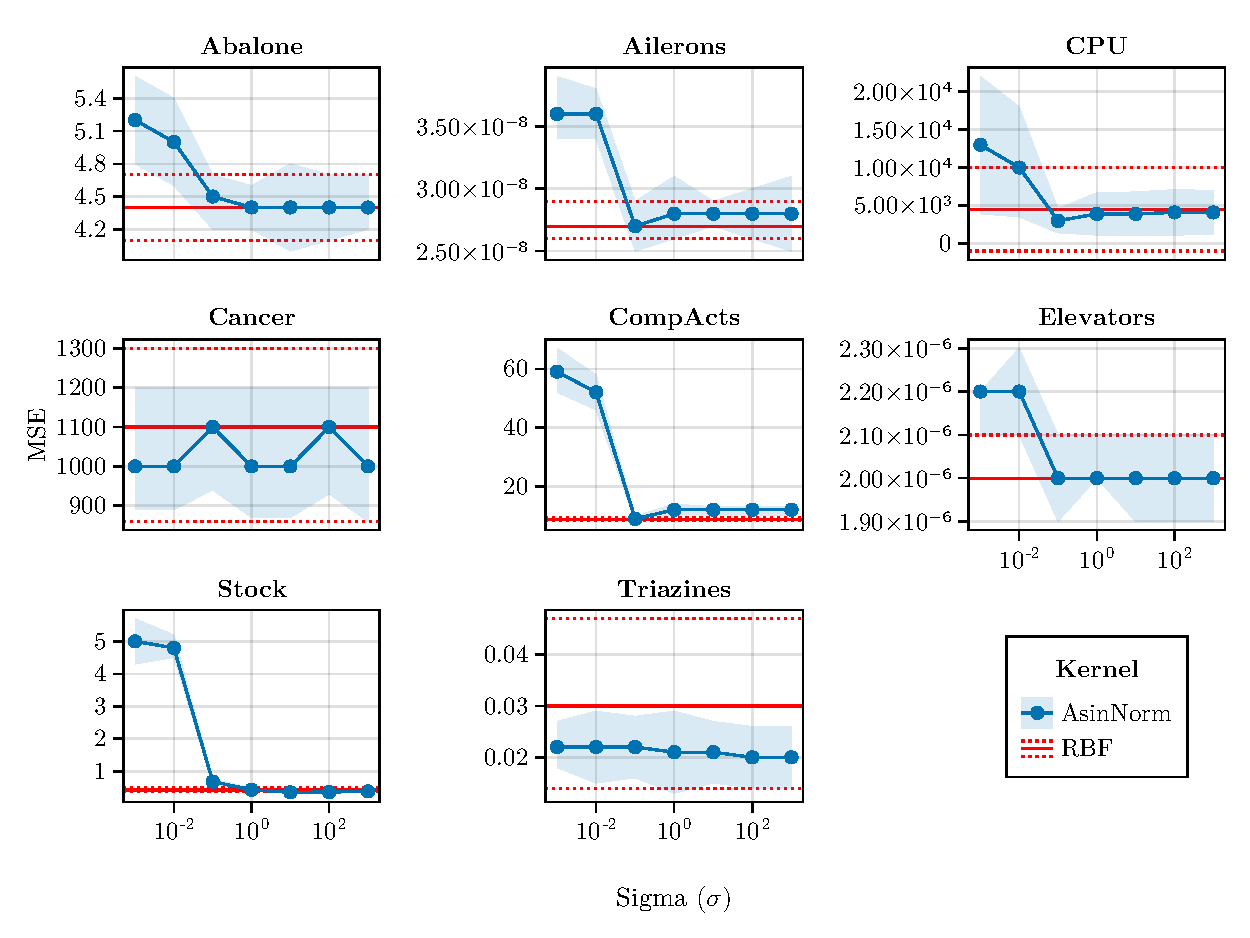
\includegraphics[width=.7\textwidth]{plots/MSE_frenay_original}
    \caption{MSE from \cite{frenayParameterinsensitiveKernelExtreme2011}}
    \label{fig:mse-frenay-original}
\end{figure}

\begin{figure}[H]
    % TODO: make color more clear
    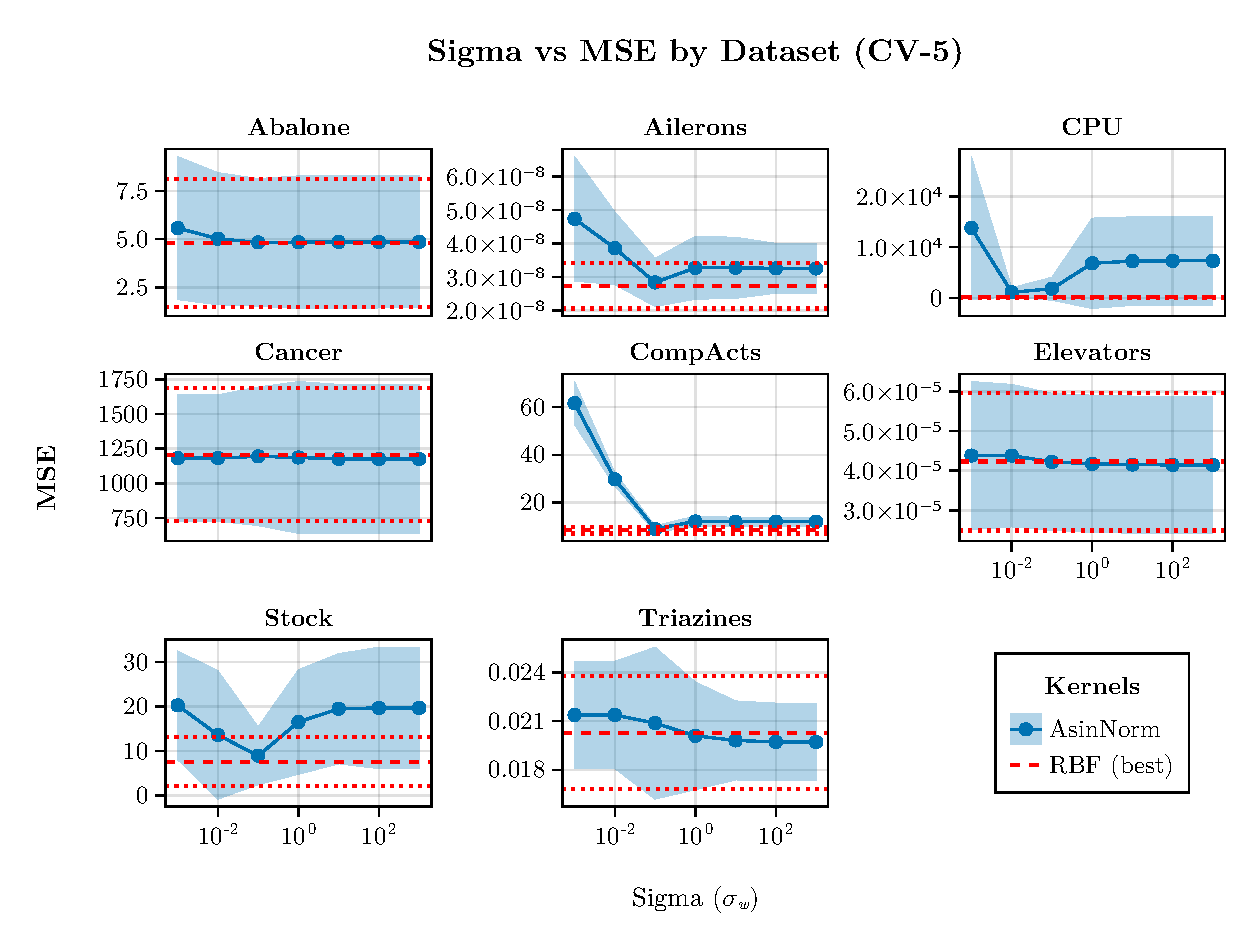
\includegraphics[width=.7\textwidth]{plots/MSE_frenay}
    \caption{Our reproduction of the results from \cite{frenayParameterinsensitiveKernelExtreme2011}}
    \label{fig:mse-frenay}
\end{figure}

\Cref{fig:mse-frenay} shows the results of the arc-sine
kernel~(normalized and non-normalized) on the same datasets used by \textcite{frenayParameterinsensitiveKernelExtreme2011}. The shading corresponds to the standard deviation when averaging the
cross-validation results.

% TODO: plots side by side so it's easier to compare
When comparing \cref{fig:mse-frenay-original} and \cref{fig:mse-frenay}, we
can see that the results are similar, but there are notable differences in some
datasets. In general, the confidence intervals are larger in our results, which
is expected since we use a different resampling method.

\begin{description}
    \item[\texttt{Abalone}] Our confidence interval is much larger and ecompases
        their whole confidence interval. Our results do not show significant difference
        for lower values of sigma as theirs does, but there is an appreciable
        difference for $\sigma_w=10^{-3}$.
    \item[\texttt{Ailerons}] The results are consistent with the original paper.
    \item[\texttt{CPU}] The behaviour is similar. The confidence interval of RBF
        is much tighter in our results.
    \item[\texttt{Cancer}] Similar to the original paper, but again the confidence
        interval of our results is significantly larger.
    \item[\texttt{CompActs}] In this case, the results are extremely similar.
    \item[\texttt{Elevators}] Our results do not exhibit the same behaviour and
        are 1 order of magnitude higher than theirs in both arc-sine and RBF. Looking
        at results on the dataset in OpenML\footnote{\url{https://www.openml.org/search?type=data&sort=runs&id=216&status=active}}, other people obtain values of RMSE between $0.0067$ and $0.0046$ which
        in MSE is between $0.000045$ and $0.000022$. These results align with ours,
        so there may be a typo in the original paper or there are using a different
        version of the dataset or some other difference in the preprocessing.
    \item[\texttt{Stock}] For this dataset, the behaviour is very different. The
        stock dataset consists of stock data from 10 companies.
    \item[\texttt{Triazines}] The behaviour is similar. As in \texttt{CPU},
        the confidence interval of RBF is much tighter in our results.
\end{description}

The datasets where the results are significantly different are \texttt{Elevators}
and \texttt{Stock}. In the case of \texttt{Elevators}, we have already discussed
that there may be some difference in the preprocessing of the dataset.

% TODO: Is this a correct interpretation?
\texttt{Stock} is a dataset of daily stock data from 10 companies. This
means that the data is not independent, and thus the resampling method used
by \textcite{frenayParameterinsensitiveKernelExtreme2011} which takes
90\% of the data for training and 10\% for testing may not be appropriate. Since
there is a high probability that the test set contains data from days that are
adjacent to the training set. Our resampling method, which uses random
50\% splits is not affected as much by this problem and thus our results are
different.


\pagebreak
\section{Arc-sine kernels}
%! TEX root = **/000-main.tex
% vim: spell spelllang=en:

\subsection{Normalized arcsine kernel}

\subsubsection{Regression}

\Cref{fig:nrmse-asinnorm-scaled} shows the obtained normalized root mean
squared error (nRMSE) for each dataset and each value of $\sigma$ for all the
regression kernels tested using the normalized arcsine kernel. We show the
\emph{nRMSE} for the best combination (the one with minimal \emph{nRMSE})
of the other hyperparameters ($C$ and $\varepsilon$) for each value of sigma.
The value for \emph{nRMSE} is the mean of the 10 folds and the shaded area
represents the 95\% confidence interval.
As a reference, we present the best results obtained by the radial basis
function (RBF) kernel as a dashed horizontal line with its corresponding
95\% confidence interval as dotted lines.

\begin{figure}[H]
    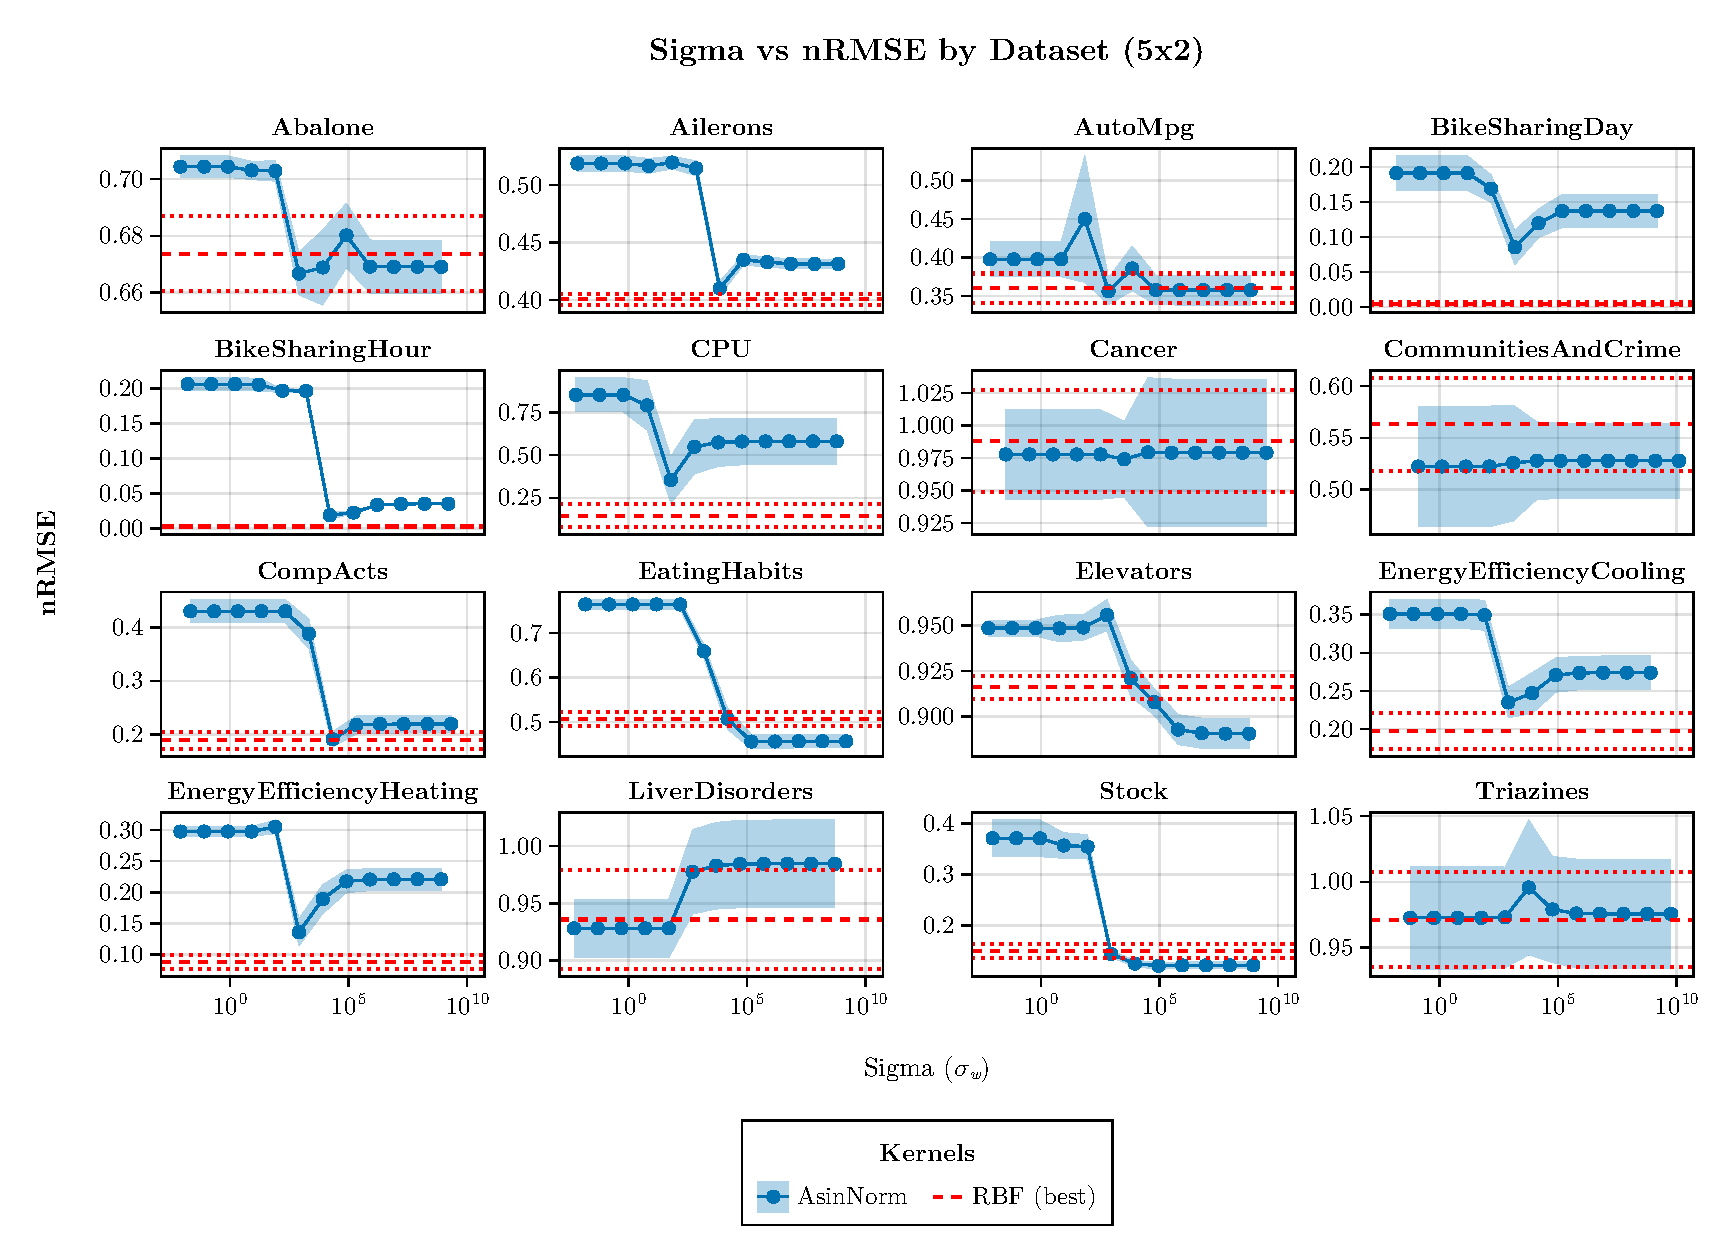
\includegraphics[width=\textwidth]{plots/nRMSE_nodelve_asinnorm_scaled_unlinked}
    \caption{Sigma vs Normalized Root Mean Squared error by dataset using Normalized arcsine kernel}%
    \label{fig:nrmse-asinnorm-scaled}
\end{figure}

From this figure we can observe some interesting results:

\begin{enumerate}
    \item Except for \texttt{BikeSharingDay} and \texttt{EnergyEfficiencyHeating},
          the normalized arcsine kernel has at least one point in which the \emph{nRMSE} is
          within the confidence interval of the RBF kernel.
    \item The kernel seems to stabilize for $\sigma \geq 10^5$. This supports
          the idea of the kernel being insensitive to the value of $\sigma$.
    \item In some cases, the normalized arcsine kernel outperforms \emph{RBF}:
          \texttt{EatingHabits}, \texttt{Elevators} and \texttt{Stock}.
    \item Looking at \texttt{Ailerons} we see that for a specific value of
          $\sigma$, the results are similar to the RBF kernel, but deviating
          from that value increases the \emph{nRMSE} significantly. This can also
          be observed in \texttt{BikeSharingHour}, \texttt{CompActs} and \texttt{EnergyEfficiencyCooling}.
\end{enumerate}

These observations hint that the kernel, although it may stabilize to the same
performance for high values of sigma, this high values of sigma may not be
optimal.

If we now look at the results for the \texttt{Delve} datasets shown in
\cref{fig:nrmse-delve-asinnorm-scaled}. In the figure, we show the results for
all 8 combinations of features (8 or 32), linearity (fairly linear or nonlinear)
and noise (moderate or high) for each of the two synthetic datasets. This
gives a total of 16 datasets.

From the Delve datasets we can further observe:
\begin{enumerate}
    \item The arcsine kernel struggles (does not reach parity with the results from RBF)
          with the Bank dataset with 32 features and moderate noise in
          both fairly linear and nonlinear cases.
    \item We observe the same pattern described in the previous plot for
          \texttt{Ailerons} in the \texttt{Delve} datasets. That is,
          there is a value of $\sigma$ which gives similar results to the RBF and
          deviating from that value increases the \emph{nRMSE}.
    \item In the high noise cases with 32 features (bottom right plot
          of each subdivision) the arcsine kernel behaves similarly to the RBF kernel
          or outperforms it (PumaDyn non-linear).
    \item In general, the best results for the arcsine kernel in relation to the
          RBF kernel are obtained in the combination of high noise and non-linear
          cases. Which are the ``hardest'' problems and arguably the ones which
          are more similar to real world problems.
\end{enumerate}

% \begin{figure}[H]
%     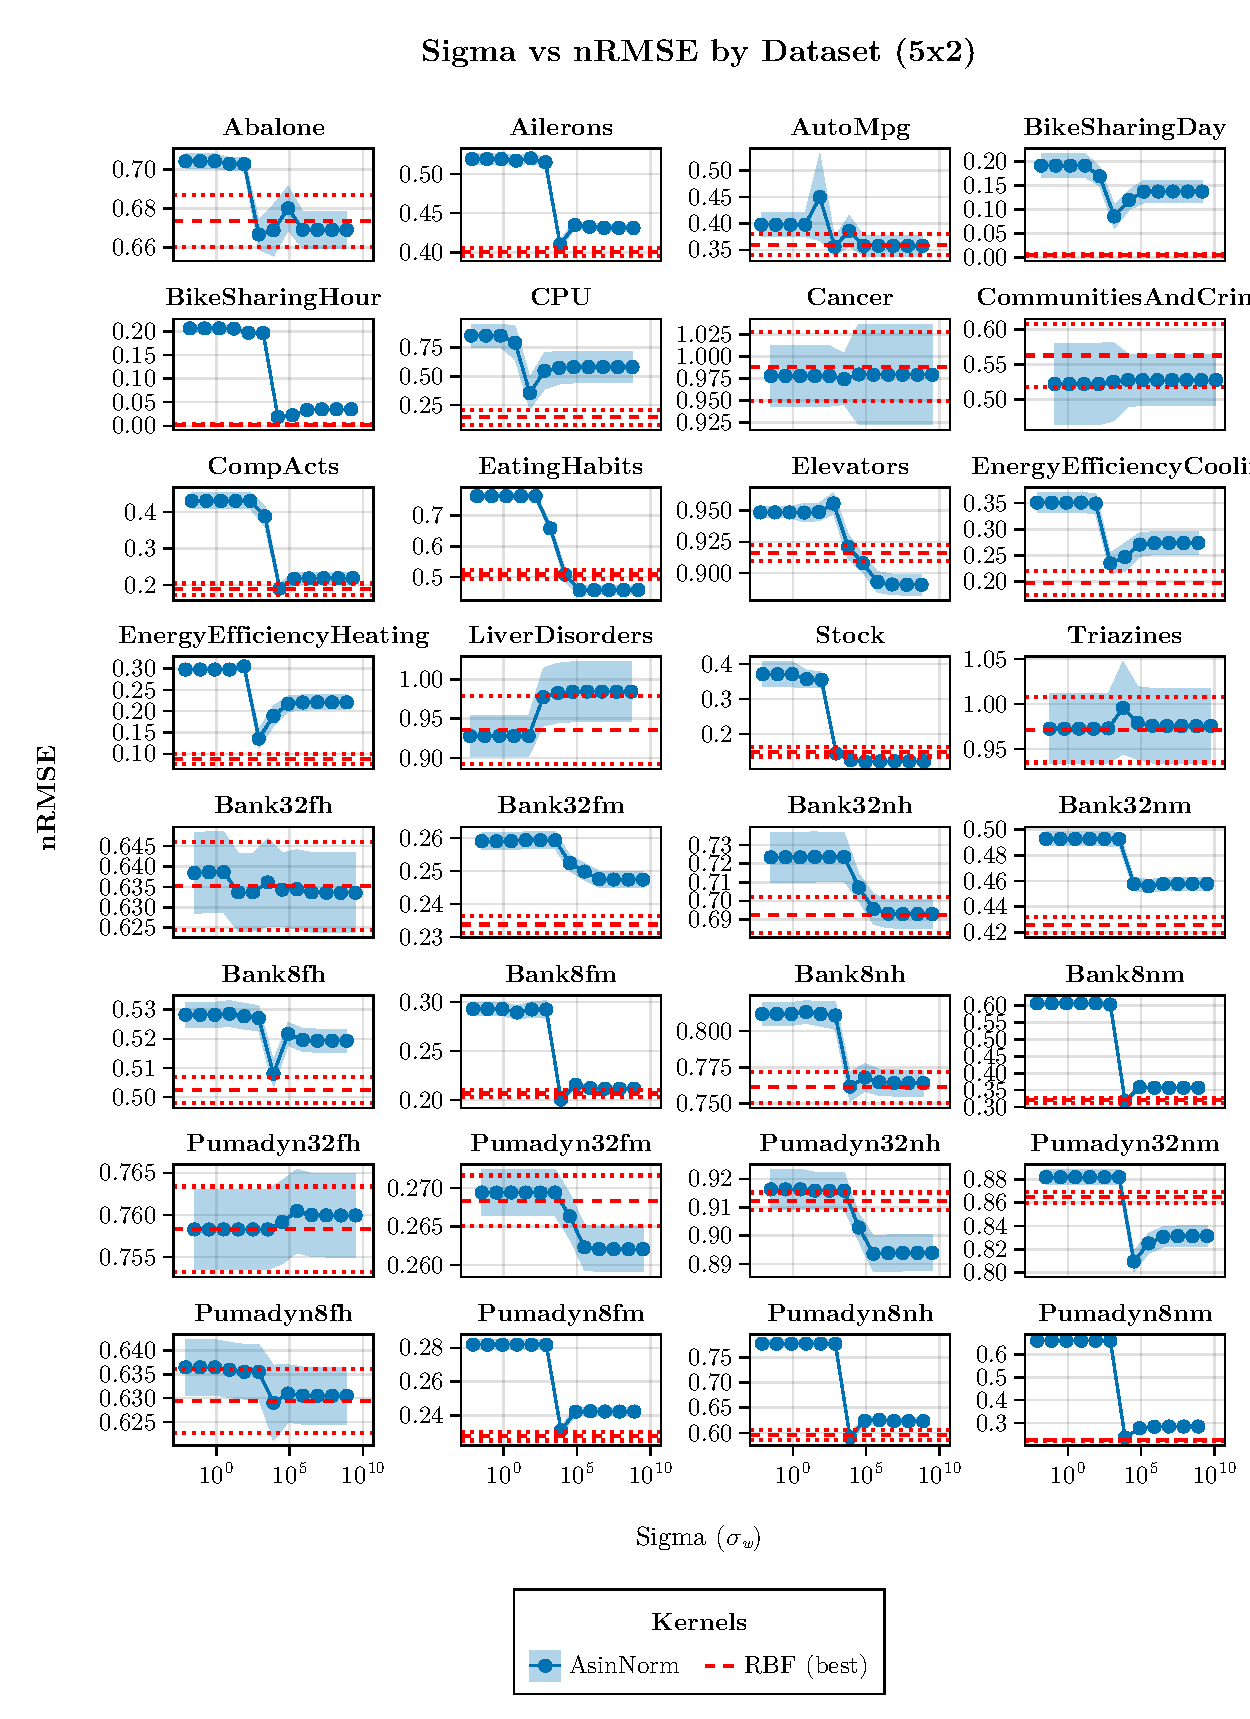
\includegraphics[width=\textwidth]{plots/nRMSE_asinnorm_scaled}
%     \caption{Sigma vs Normalized Root Mean Squared error by dataset using Normalized arcsine kernel}%
%     \label{fig:nrmse-asinnorm-scaled}
% \end{figure}

% \begin{figure}[H]
%     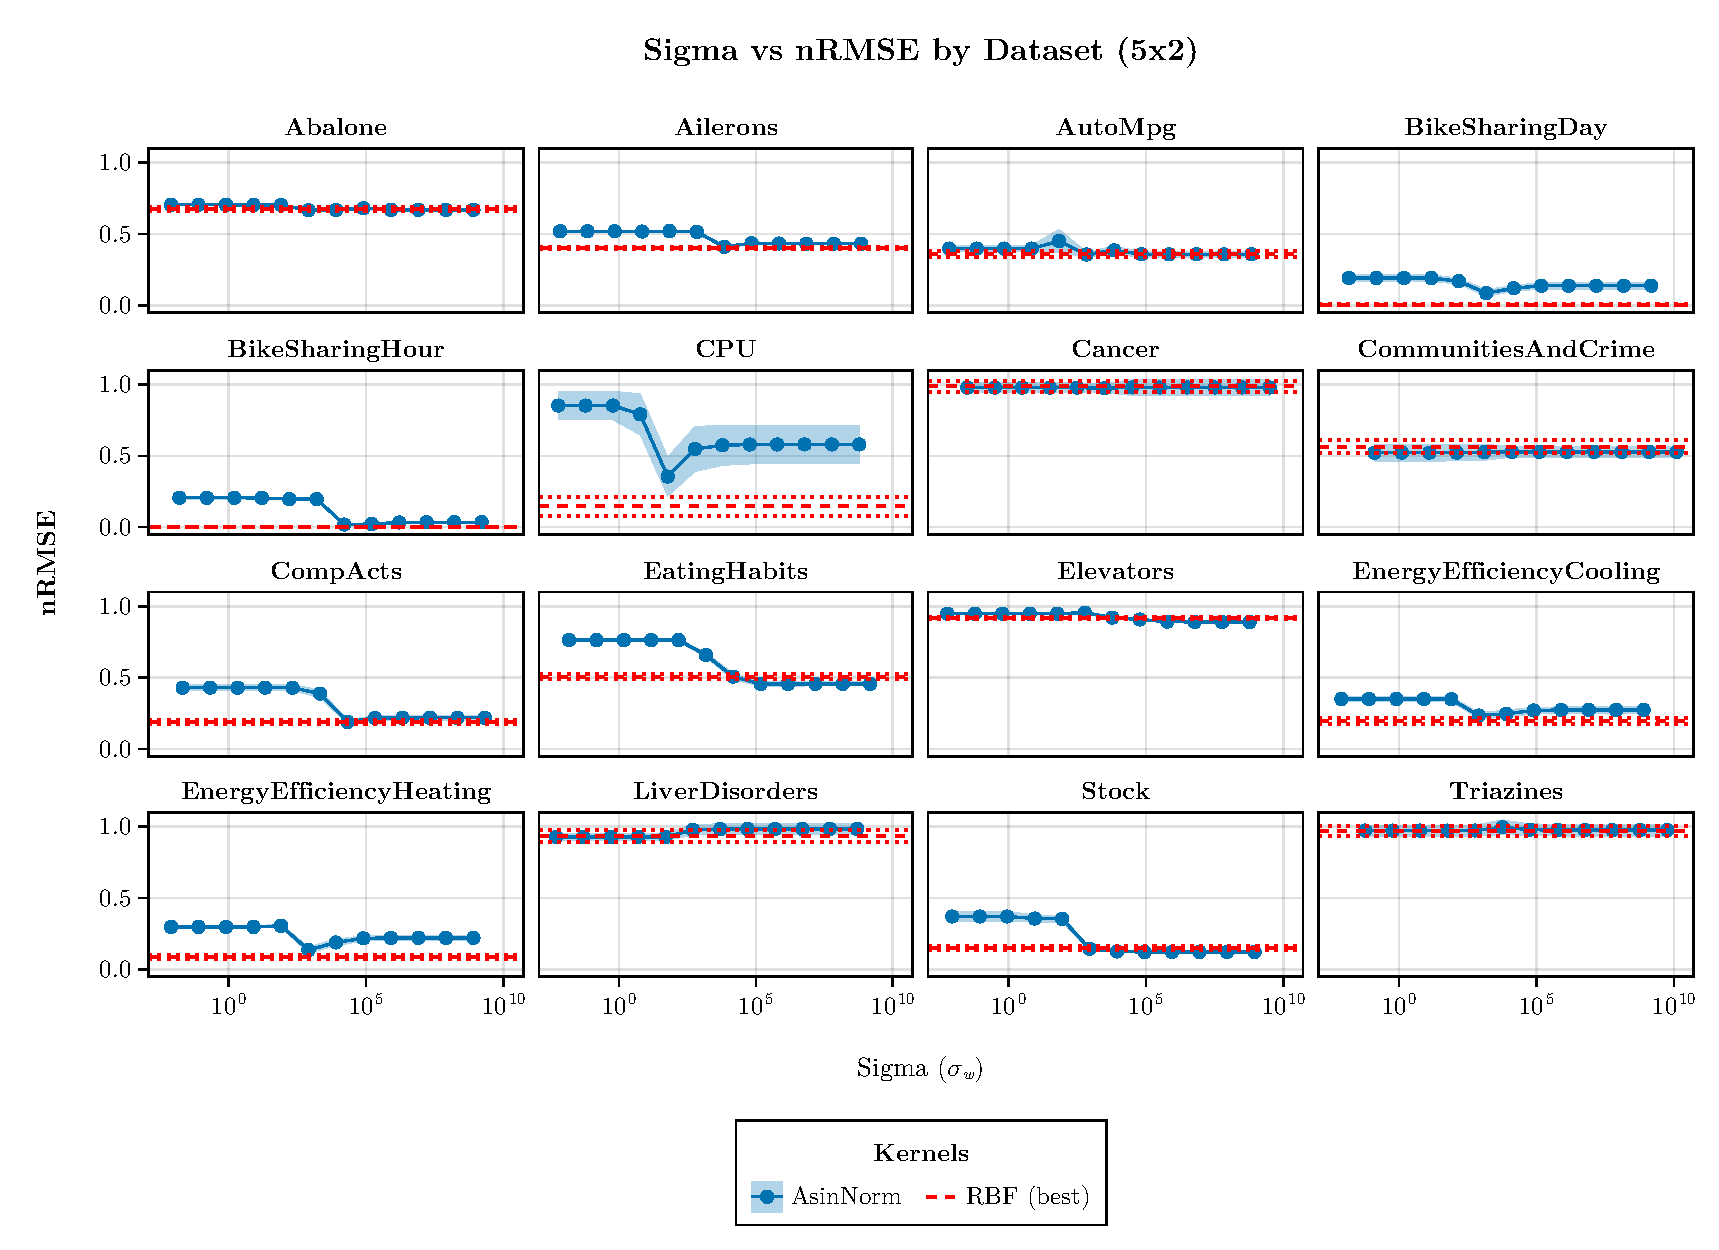
\includegraphics[width=\textwidth]{plots/nRMSE_nodelve_asinnorm_scaled}
%     \caption{Sigma vs Normalized Root Mean Squared error by dataset using Normalized arcsine kernel}%
%     \label{fig:nrmse-asinnorm-scaled}
% \end{figure}

% \begin{figure}[H]
%     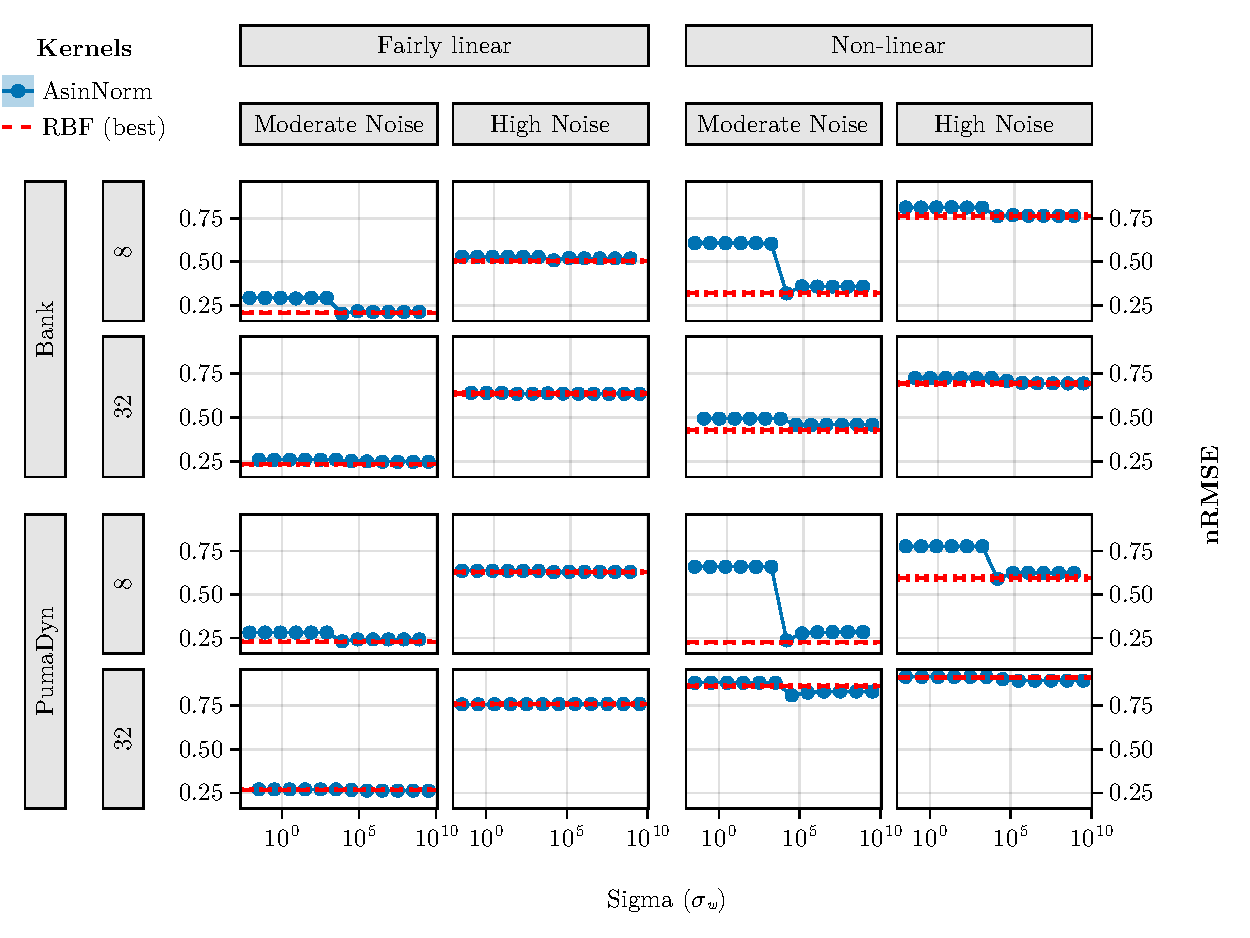
\includegraphics[width=\textwidth]{plots/nRMSE_delve_asinnorm_scaled}
%     \caption{Sigma vs Normalized Root Mean Squared error by dataset using Normalized arcsine kernel}%
%     \label{fig:nrmse-delve-asinnorm-scaled}
% \end{figure}

\begin{figure}[H]
    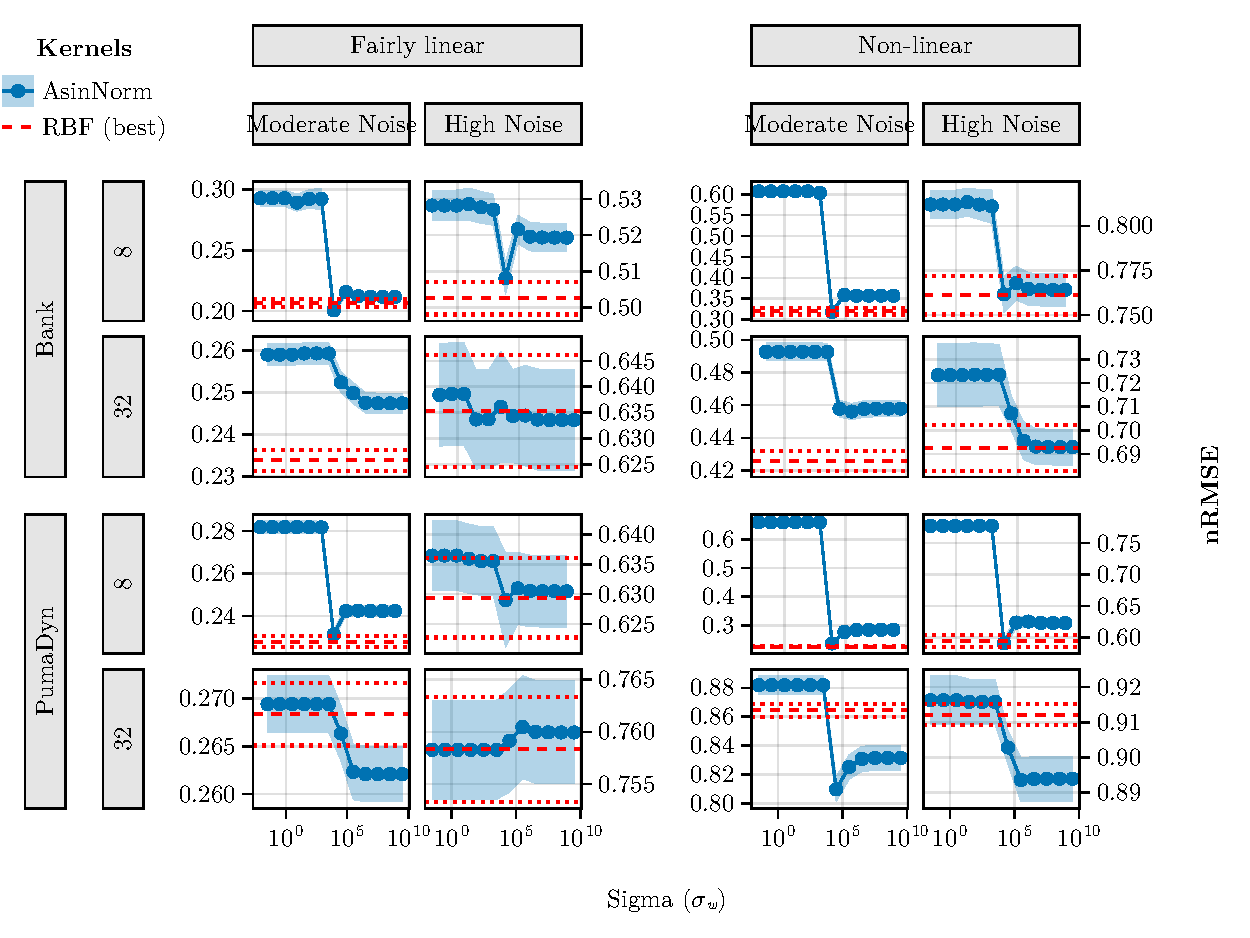
\includegraphics[width=\textwidth]{plots/nRMSE_delve_asinnorm_scaled_unlinked}
    \caption{Sigma vs Normalized Root Mean Squared error by dataset using Normalized arcsine kernel}%
    \label{fig:nrmse-delve-asinnorm-scaled}
\end{figure}

\subsubsection{Classification}

\Cref{fig:accuracy-asinnorm-scaled} shows the obtained accuracy for each
of our classification datasets. Only \texttt{Adult} and \texttt{GlassIdentification}
differ from the results obtained by the RBF kernel. In the case of \texttt{Adult},
we can clearly see a point in which the accuracy reaches parity with the RBF
kernel. For $10^5$ it obtains the best accuracy and further increasing the sigma
stabilizes slightly below the RBF kernel (but inside the confidence interval). For
\texttt{GlassIdentification} there is a drop in accuracy with higher values of
sigma, which is not what we expected. A similar behaviour can be observed in
\texttt{Iris} to a lesser extent. It is unclear why this happens.

% TODO: glass why?

\begin{figure}[H]
    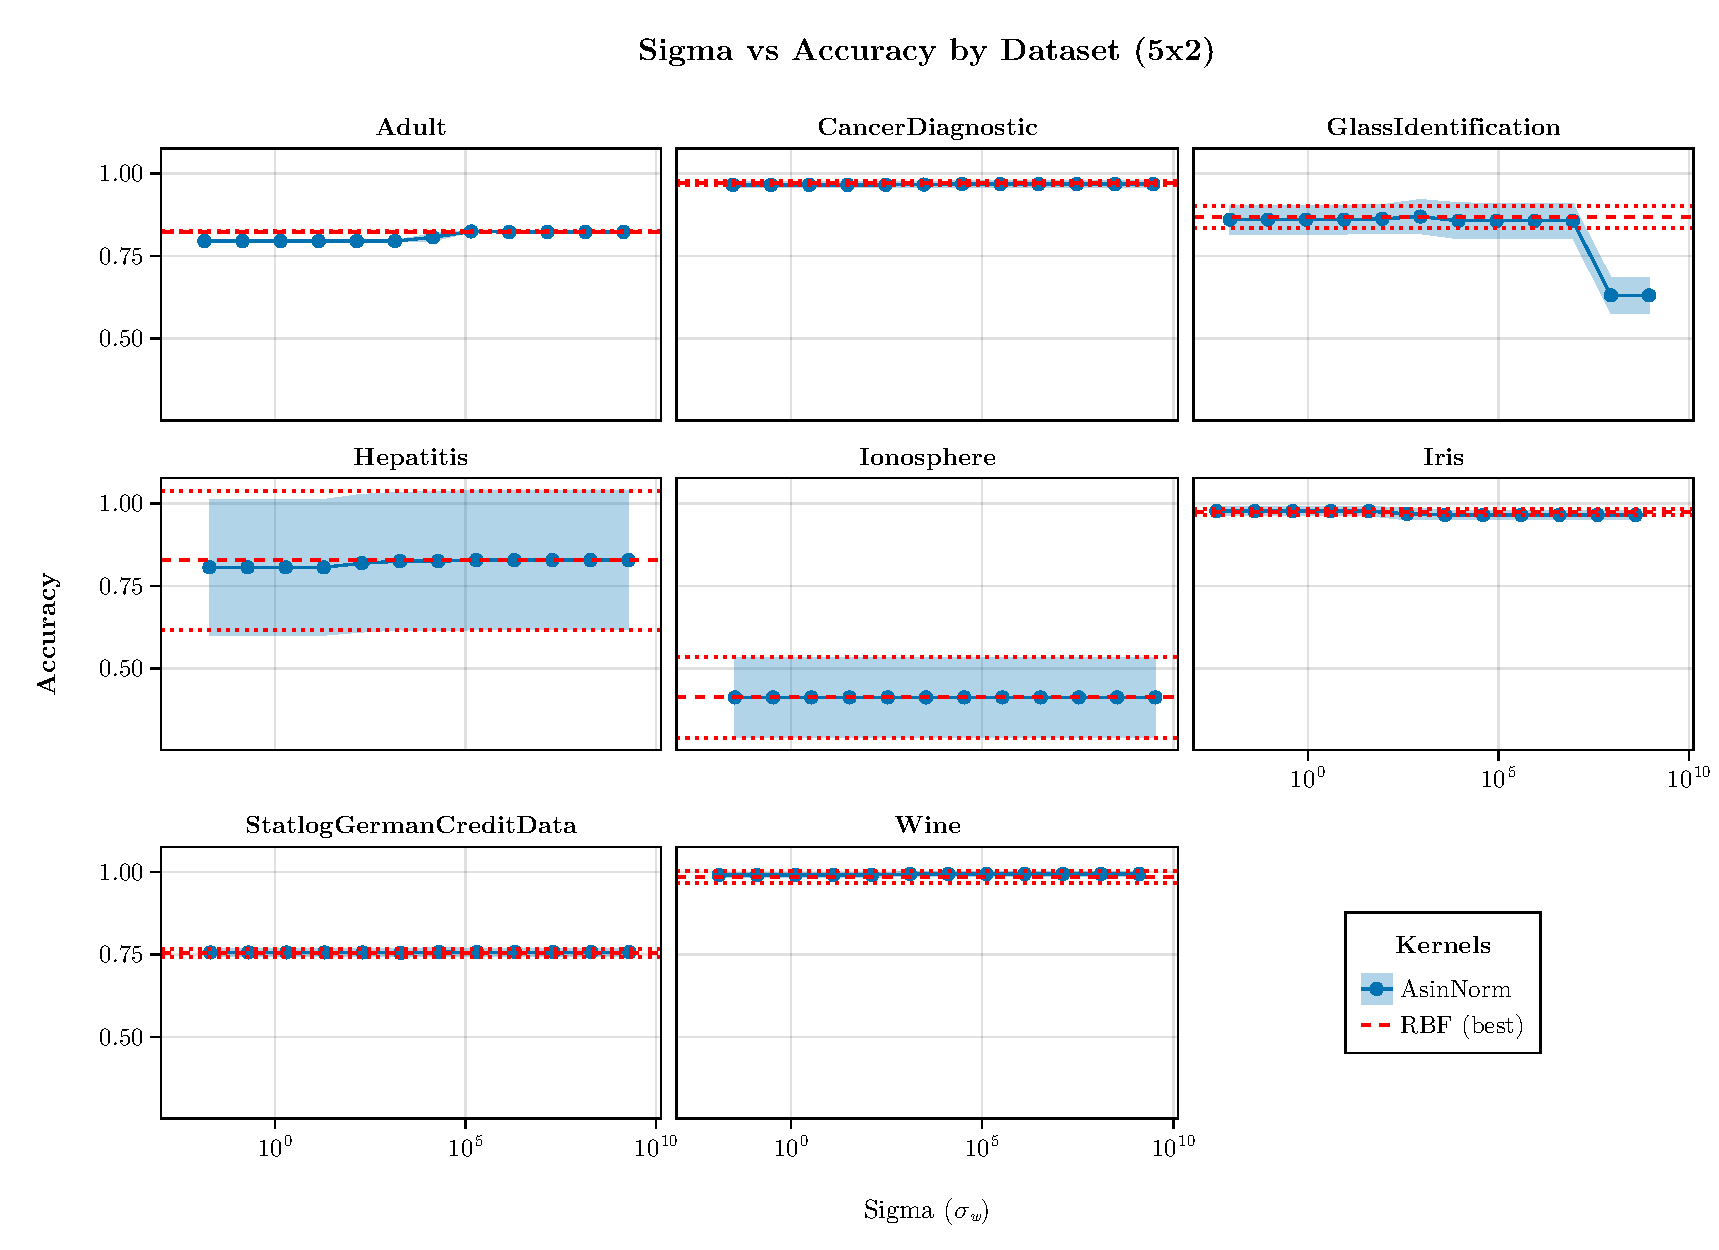
\includegraphics{plots/accuracy_class_asinnorm_scaled}
    \caption{Sigma vs Accuracy by dataset using Normalized arcsine kernel}%
    \label{fig:accuracy-asinnorm-scaled}
\end{figure}

\subsubsection{Comparison with radial basis (RBF) kernel}

The statements made in the previous sections, hint that the normalized arcsine
kernel are based on observations of the different plots presented. However,
without some statistical analysis, we cannot draw any meaningful conclusions
beyond that. In this section, we will perform the paired t-test as described in
\cref{sec:paired-t-test} to assess whether the differences in performance which
we observe are statistically significant or are just anecdotal.


In particular, we are interested in how
the sigma parameter affects the performance of the kernel. For this reason,
we compare the different values of sigma for the arc-sine kernel against the
values of gamma for the RBF kernel.

For each dataset, $\sigma$ and $\gamma$ combination we perform a paired t-test
against the best combination of hyperparameters ($C$ and $\varepsilon$) for
each kernel. \Cref{fig:paired-ttest-rbf-asinnorm} shows the $p$\textendash{}values
obtained for these paired t-test results. The darker the color, the lower the
$p$\textendash{}value and the more significant the difference between the two
kernel configurations.

\begin{figure}[H]
    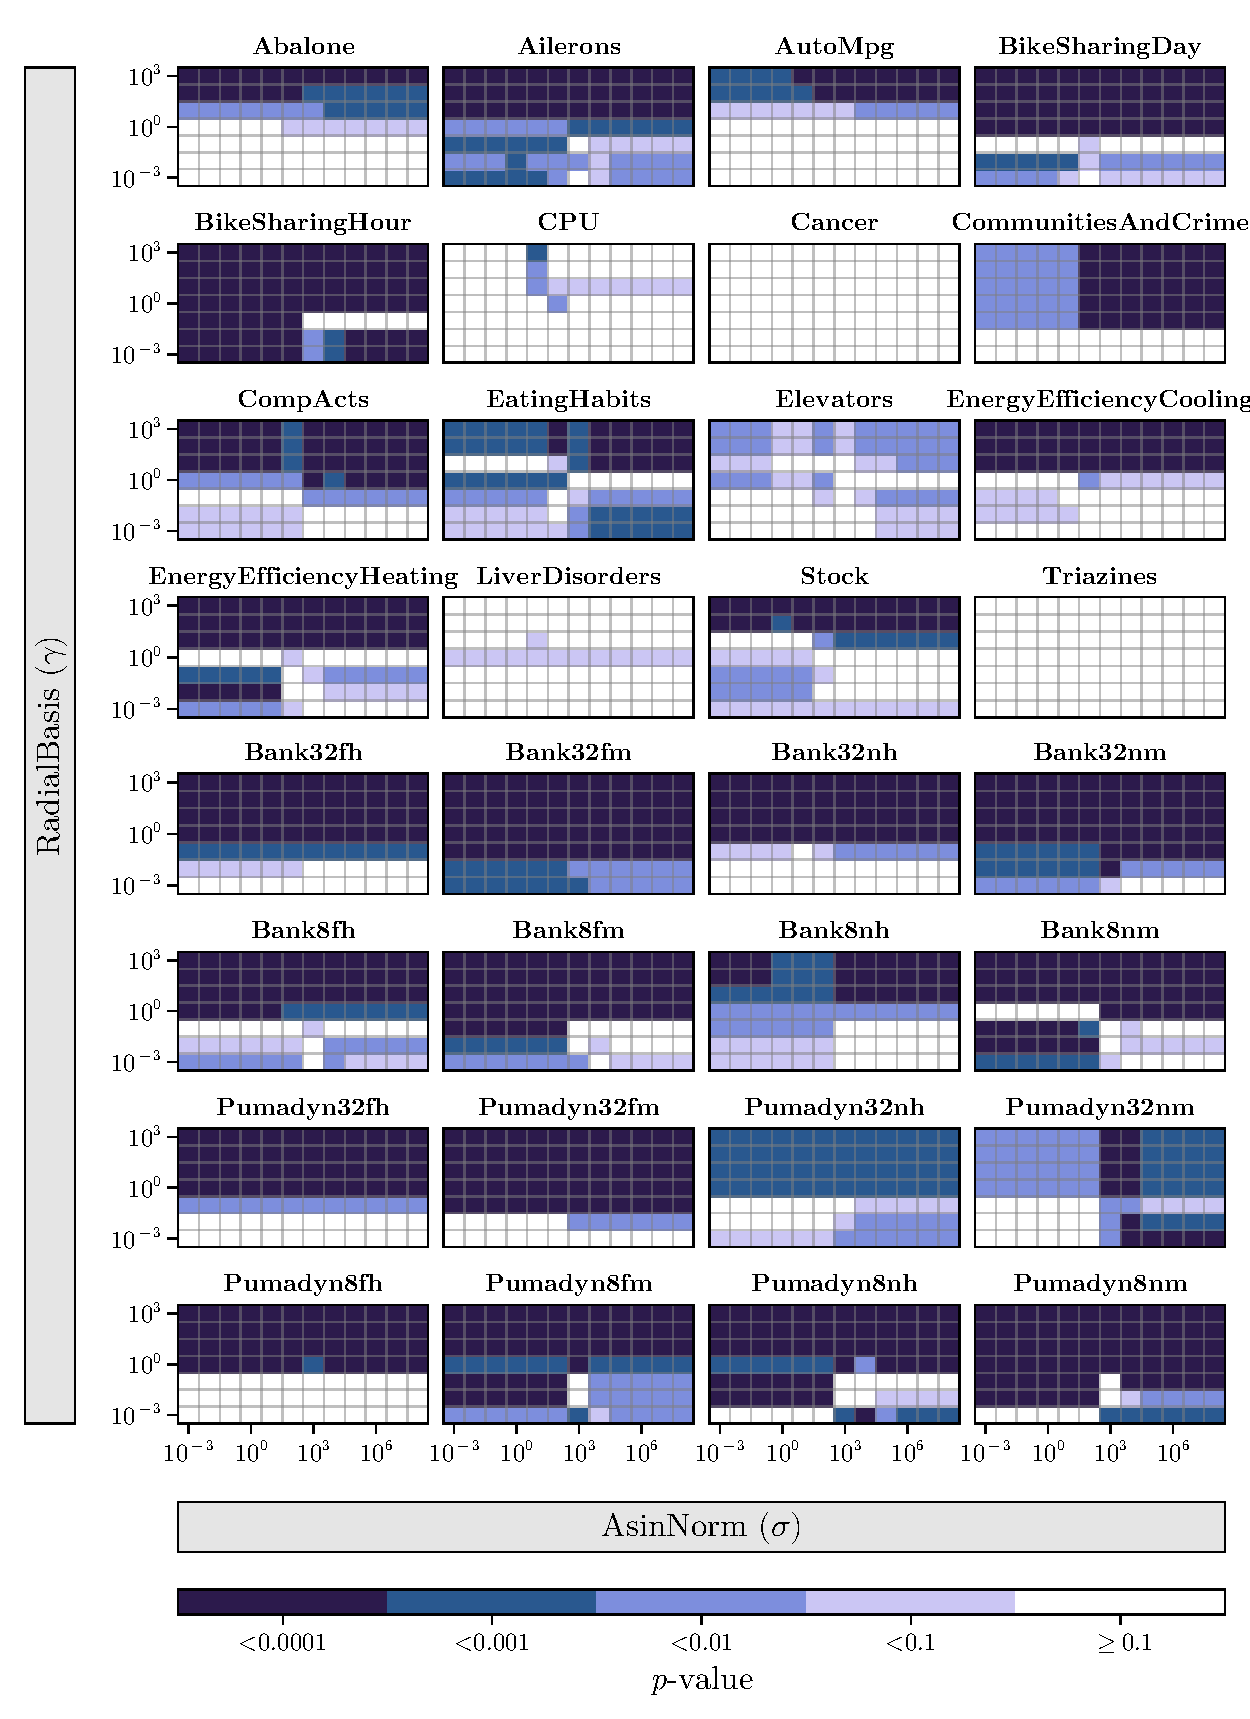
\includegraphics[width=0.9\textwidth]{plots/heatmaps_rbf_asinnorm_pvalues}
    \caption{p values}
    \label{fig:paired-ttest-rbf-asinnorm}
\end{figure}

From \cref{fig:paired-ttest-rbf-asinnorm} we can observe that:
\begin{enumerate}
    \item \texttt{Cancer}, \texttt{Triazines} \texttt{LiverDisorders}, and \texttt{Elevators} do not
          show significant differences between the kernels at any value of sigma or gamma.
    \item Other datasets such as \texttt{PumaDyn32fh} show no variation across the different
          values of sigma, which indicates that changing sigma has no effect on the
          relative performance of the kernel against the RBF kernel for those datasets.
\end{enumerate}

The patterns shown in the $p$\textendash{}values are not very useful since they
don't show the magnitude of the difference between the two kernels, nor do they
show the direction of the difference. For this reason, in \cref{fig:paired-ttest-rbf-asinnorm-diff}
we show the difference between the nRMSE of the RBF kernel and the normalized arcsine
kernel. The darker the color, the larger the difference between the two kernels. Red
values indicate that RBF performs better than the normalized arcsine kernel and blue
values indicate that the normalized arcsine kernel performs better than the RBF kernel.
All values that are outside the significance level $\alpha=0.001$ (that is, the
$p$\textendash{}value is higher than $\alpha$) have been removed and are shown as
white. Note that the $0$ in the colorscale is not pure white, but grey.

%  TODO: add pattern or something so the color can be seen in b/w
\begin{figure}[H]
    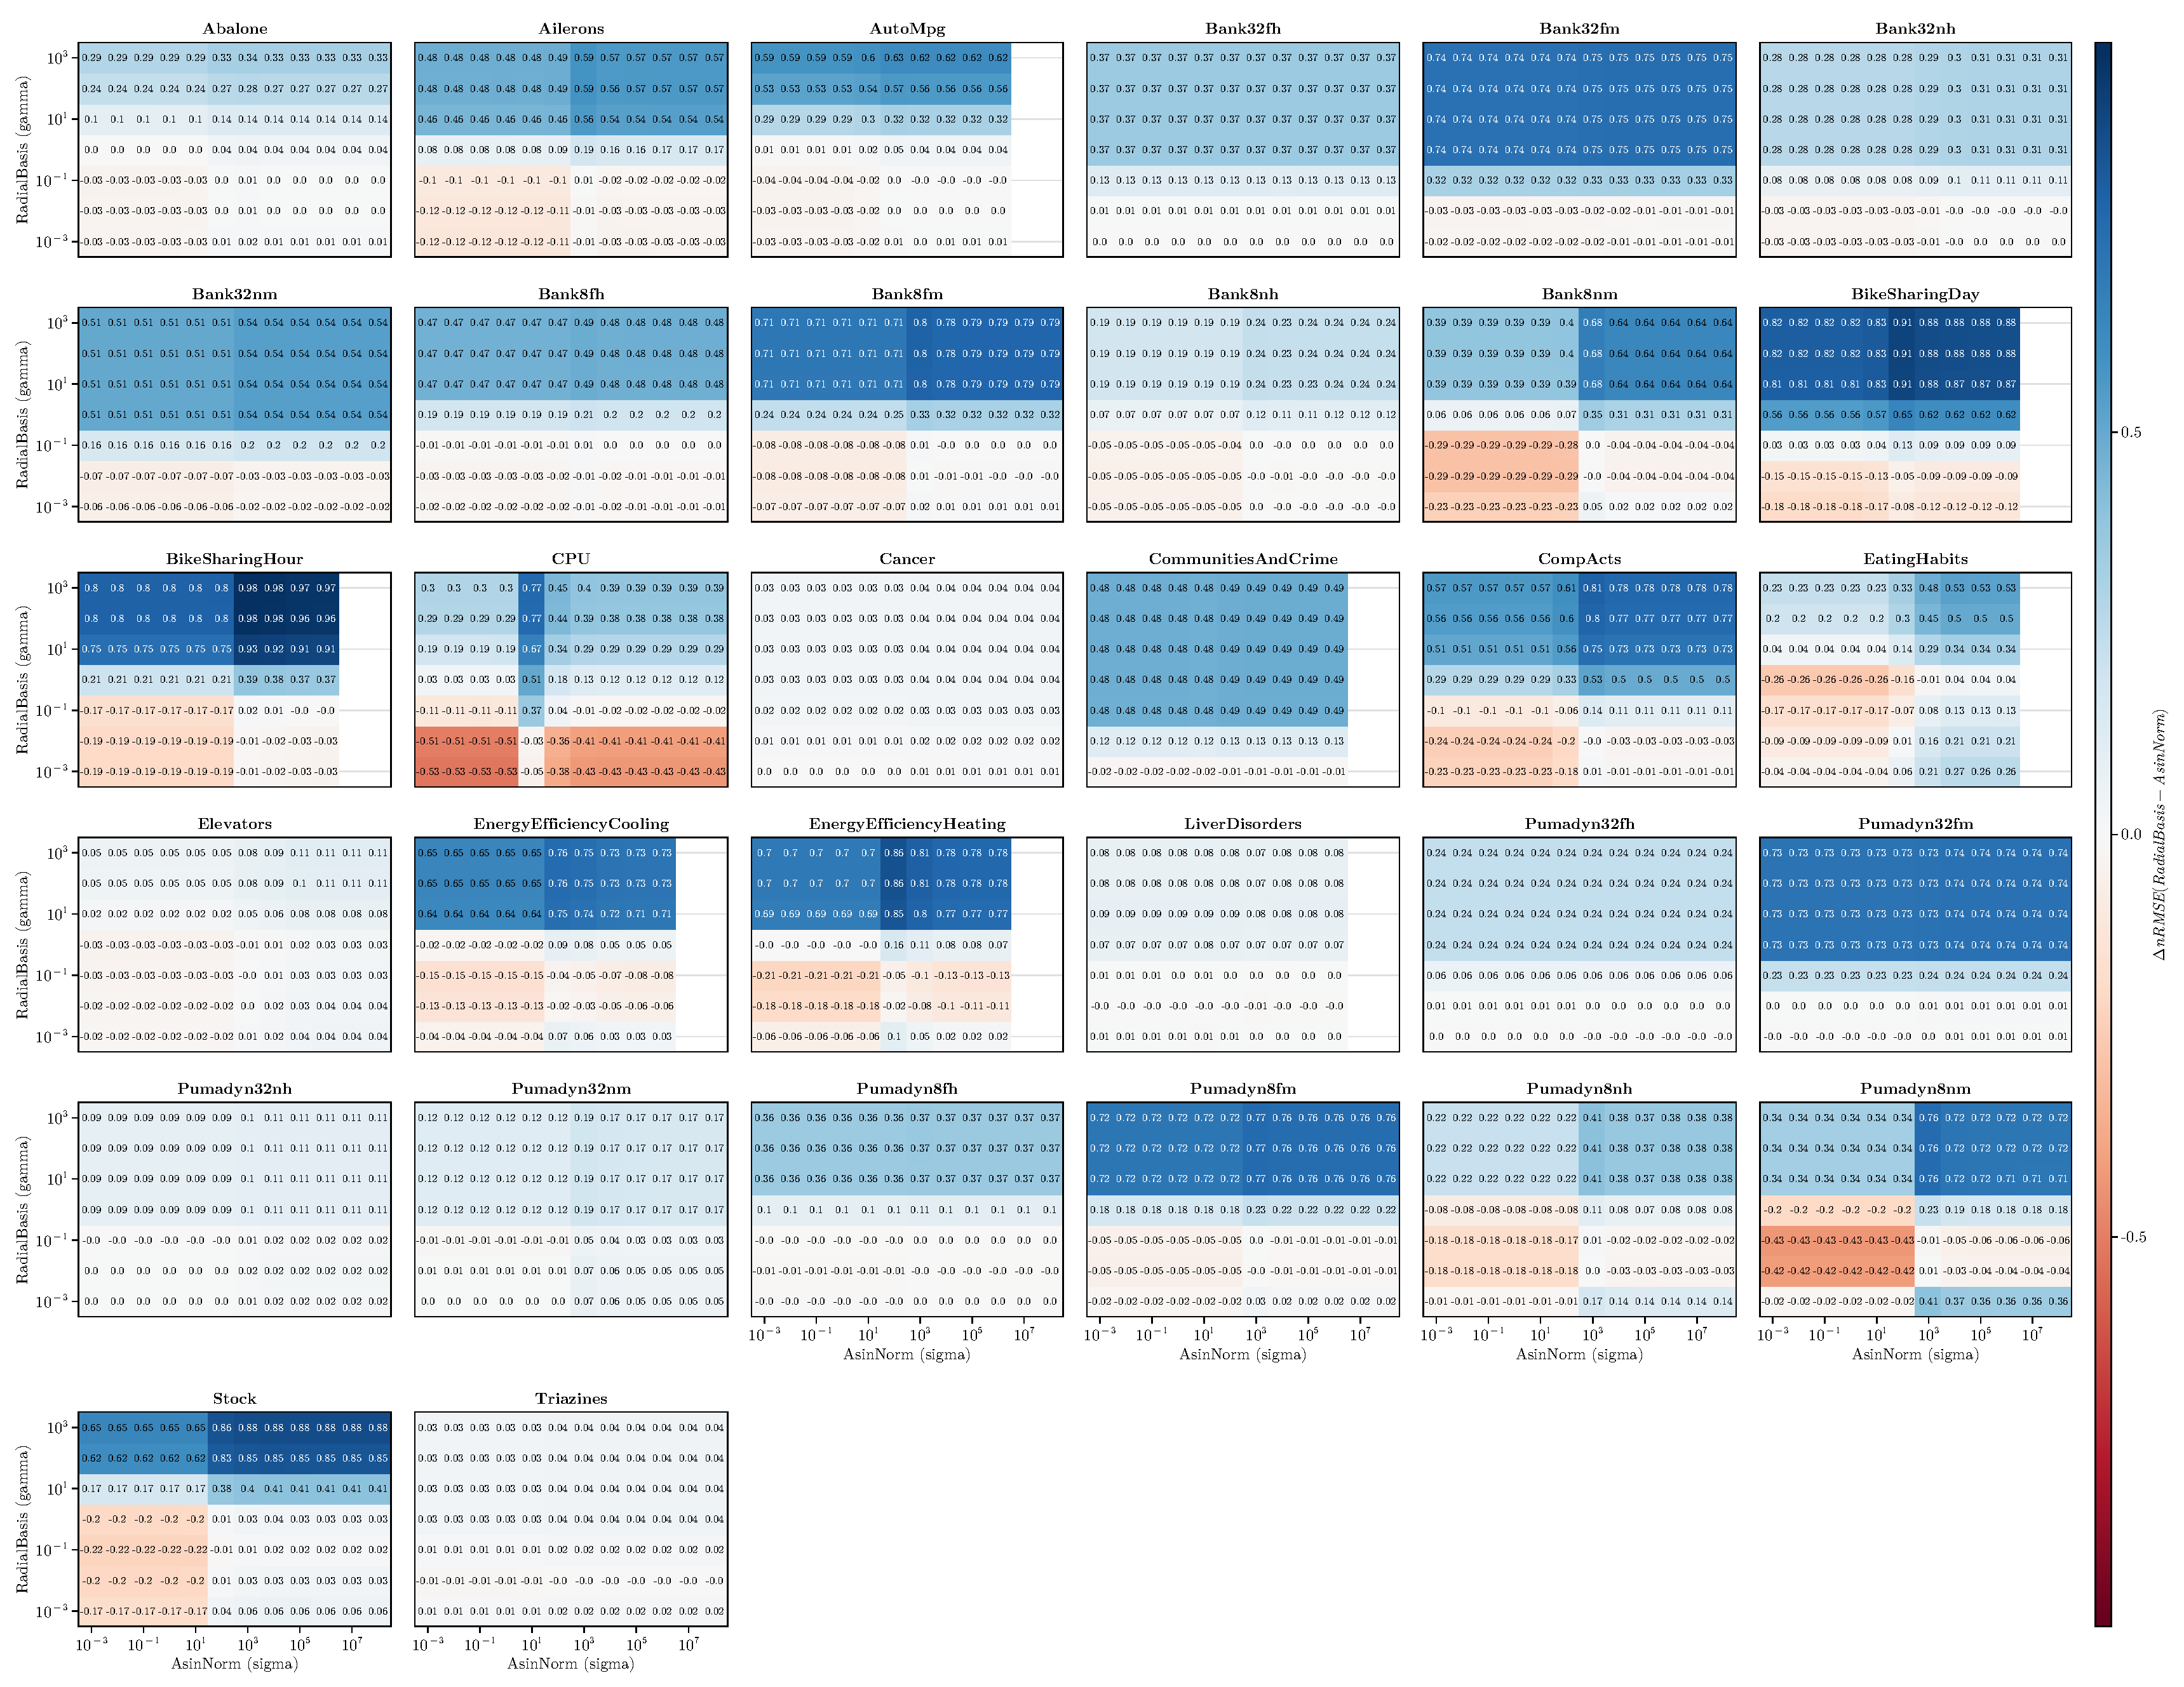
\includegraphics[width=0.9\textwidth]{plots/heatmaps_rbf_asinnorm}
    \caption{Difference between nRMSE of RBF and normalized arc-sine kernels ($\alpha=0.001$)}
    \label{fig:paired-ttest-rbf-asinnorm-diff}
\end{figure}

The way we interpret \cref{fig:paired-ttest-rbf-asinnorm-diff} is based on whether
we can see a value of sigma in which all the values to its right are blue or white.
Meaning that the normalized arcsine kernel performs better (blue) or there is no
statistically significant difference (white). All datasets except
\texttt{PumaDyn8nm} and \texttt{BikeSharingHour} show this behaviour.

In both \texttt{PumaDyn8nm} and \texttt{BikeSharingHour} we can see that all
differences for $\sigma=10^3$, are either positive (favoring the Asin kernel) or
not statistically significant, whilst for values higher there is a mix of positive
and negative values. This indicates that for $10^3$ the normalized arcsine kernel
reaches parity with the RBF kernel and for higher values of sigma, the performance
of the normalized arcsine kernel is not as good as the RBF kernel. Looking
at the previous plots (\cref{fig:nrmse-asinnorm-scaled,fig:nrmse-delve-asinnorm-scaled})
we can see that this is one of the cases in which we described the behaviour of
an ``optimal'' value of sigma which loses performance in both directions.

\subsubsection{Computational Cost}

It is difficult to compare the computational cost between the RBF kernel
and the normalized arcsine kernel. Since their performance is dependant
on the parameter selection and the dataset. \Cref{fig:time-asinnorm-scaled-compacts}
shows the boxplots of all executions of the normalized arcsine and rbf kernels
on the \texttt{CompActs} dataset grouped by the cost hyperparameter.

\begin{figure}[H]
    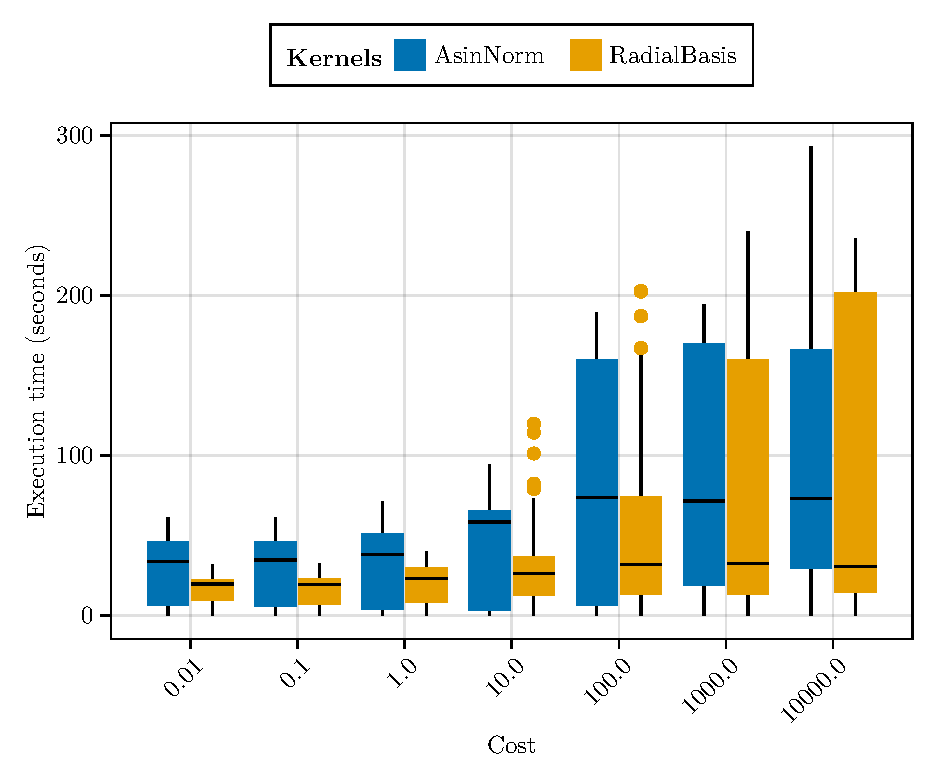
\includegraphics{plots/exec_cost}
    \caption{Time by cost parameter for normalized arcsine kernel on CompActs dataset}
    \label{fig:time-asinnorm-scaled-compacts}
\end{figure}

We can see that the cost hyperparameter has a significant effect on the
computational cost of both kernels. However, there is still a lot of variation
which comes from the effect of other hyperparameters, the data and even the
environment in which the experiments were run.

Instead, we can compute the ``speedup'' of the normalized arcsine kernel
in relation to the RBF kernel. That is, the ratio between the time taken
by the RBF kernel and the normalized arcsine kernel:
\begin{equation}
    \text{speedup} = \frac{T_{\text{RBF}}}{T_{\text{Asin}}} \label{eq:speedup}
\end{equation}
if the speedup is greater than 1, it means that the normalized arcsine kernel
is faster than the RBF kernel. If it is less than 1, it means that the RBF
kernel is faster than the normalized arcsine kernel. Since there are a lot
of outliers, we use the median instead of the mean to compute the speedup. We
do so by taking the median execution time for configuration of dataset, kernel
and hyperparameters across all folds and values of sigma and gamma and computing
the speedup using \cref{eq:speedup} for each one. Averaging these speedups
gives us a speedup of $0.68$, which means that the RBF kernel is faster by
a factor of $1/0.68 = 1.47$.

%! TEX root = **/000-main.tex
% vim: spell spelllang=en:

\subsection{Non-Normalized arcsine kernel}

Now, we will introduce the non-normalized arcsine kernel, and compare it with
both the normalized arcsine kernel and the radial basis kernel.

\subsubsection{Regression}



\begin{figure}[H]
    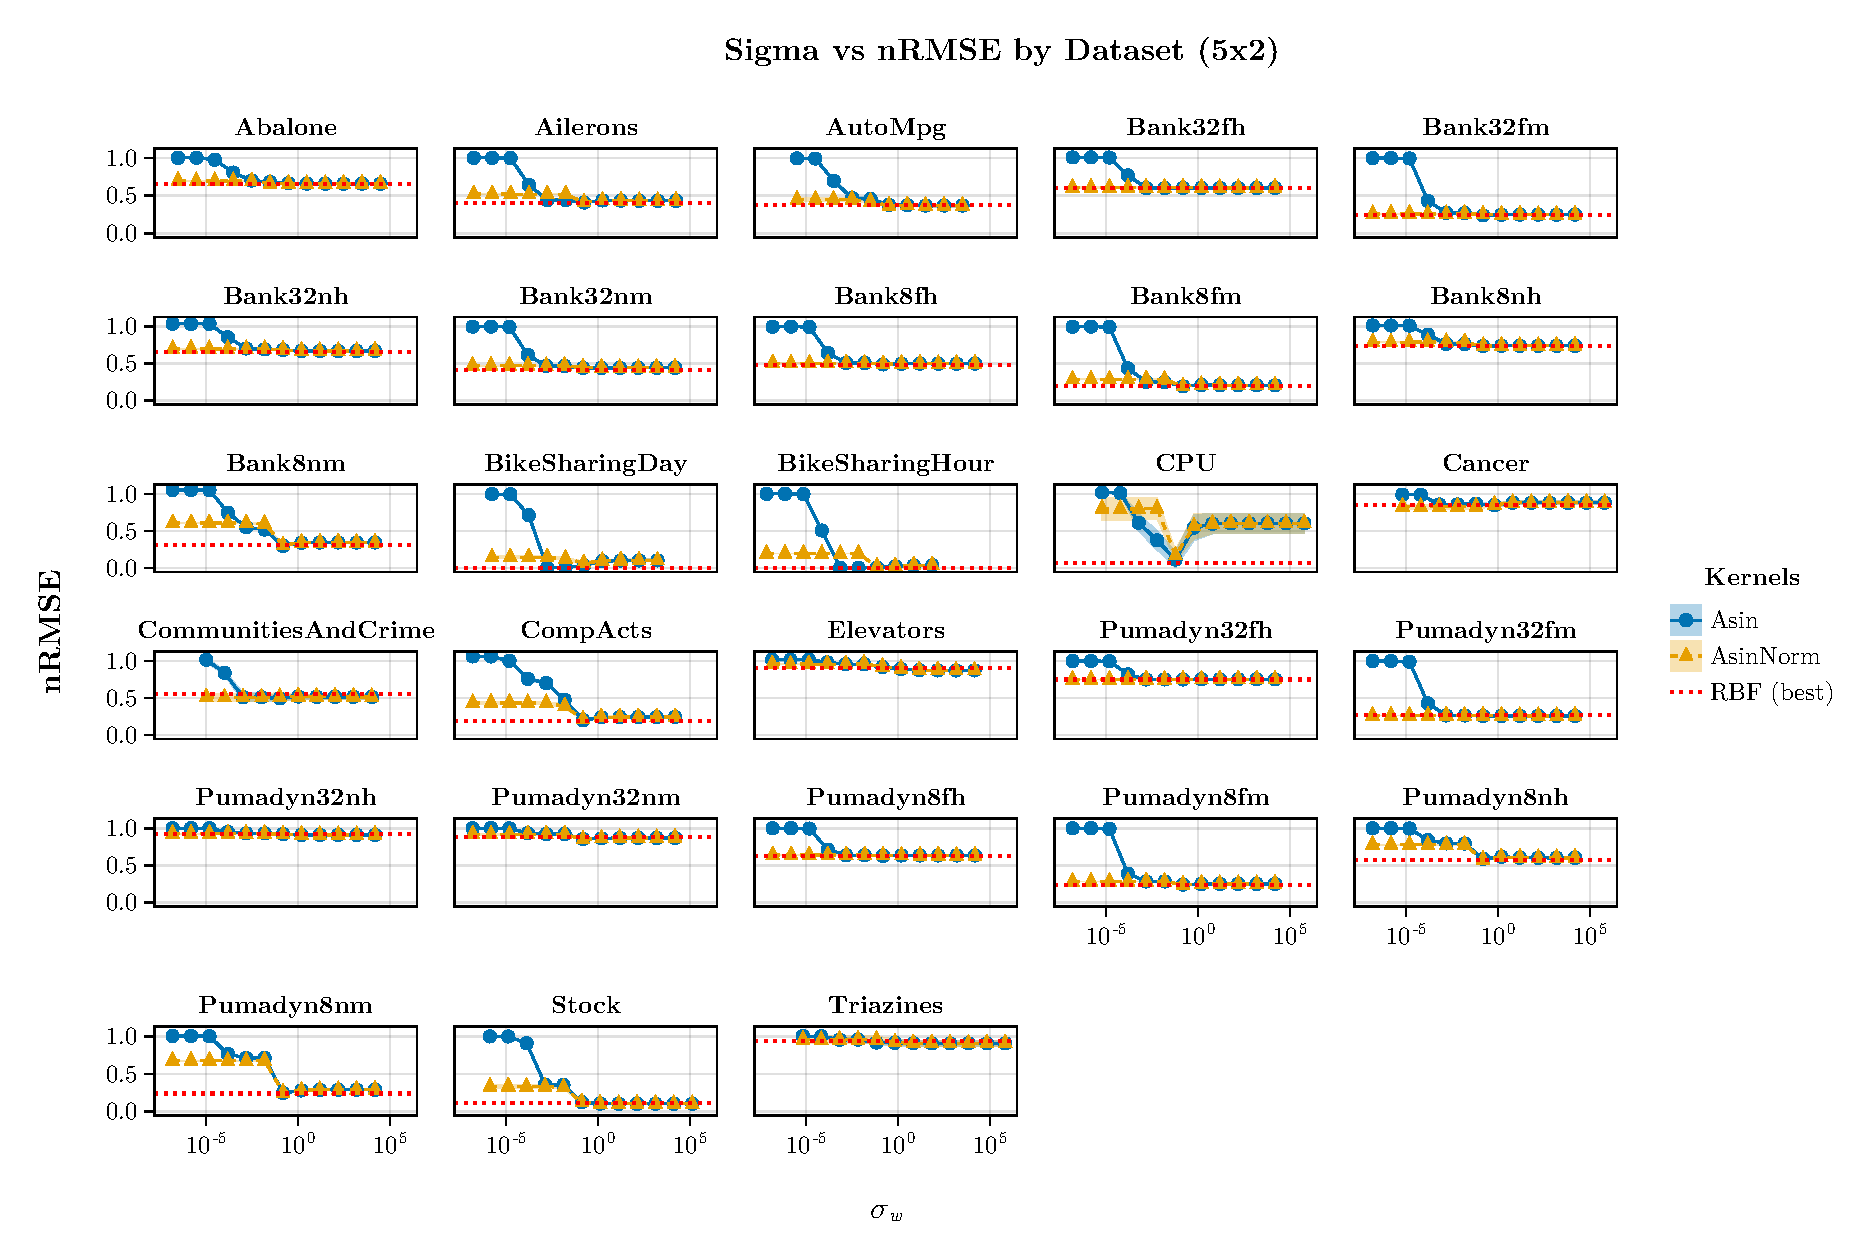
\includegraphics{plots/nRMSE_all_scaled}
    \caption{Sigma vs Normalized Root Mean Squared error by dataset using Normalized arcsine kernel}%
    \label{fig:nrmse-all-scaled}
\end{figure}

\begin{figure}[H]
    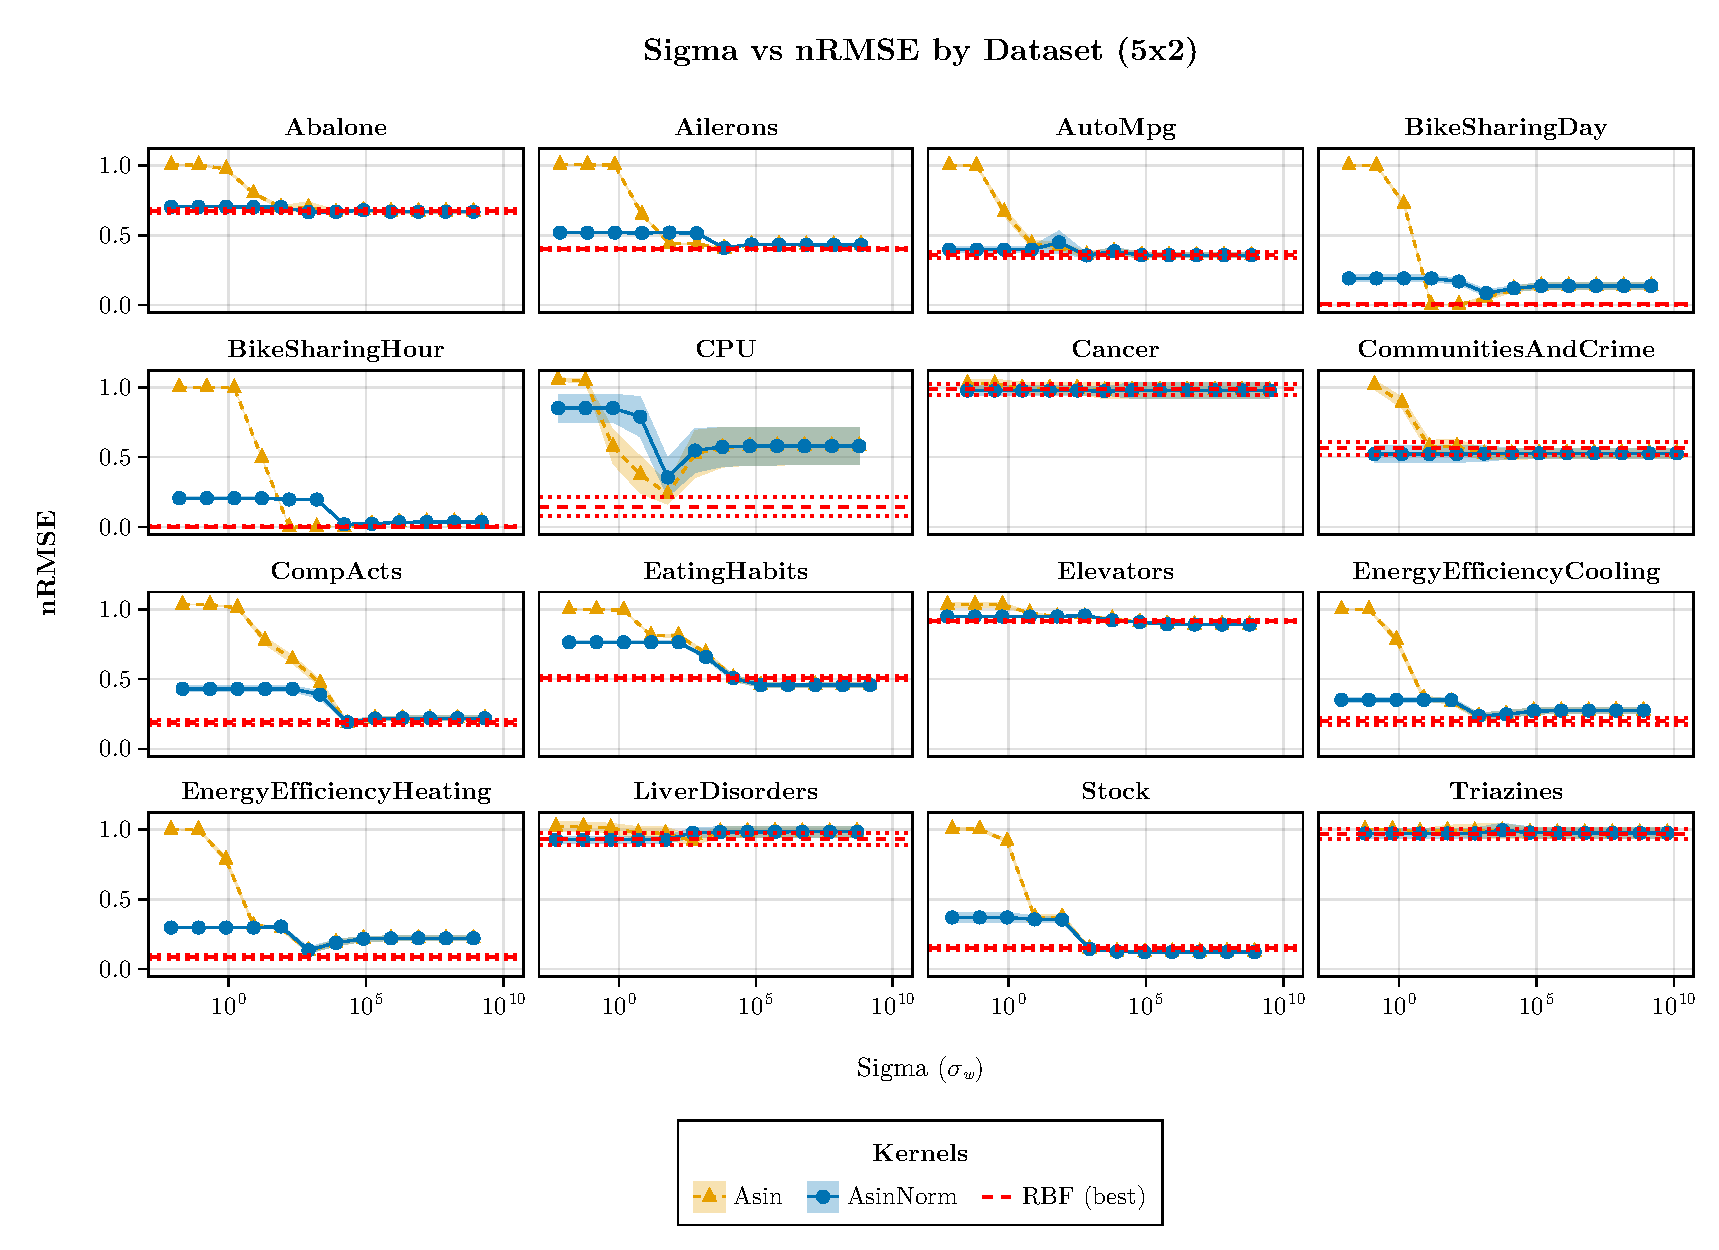
\includegraphics{plots/nRMSE_nodelve_all_scaled}
    \caption{Sigma vs Normalized Root Mean Squared error by dataset using Normalized arcsine kernel}%
    \label{fig:nrmse-all-scaled}
\end{figure}

\paragraph{Bank Delve Dataset}

% TODO: Facet all delve datasets into a single one.

\begin{figure}[H]
    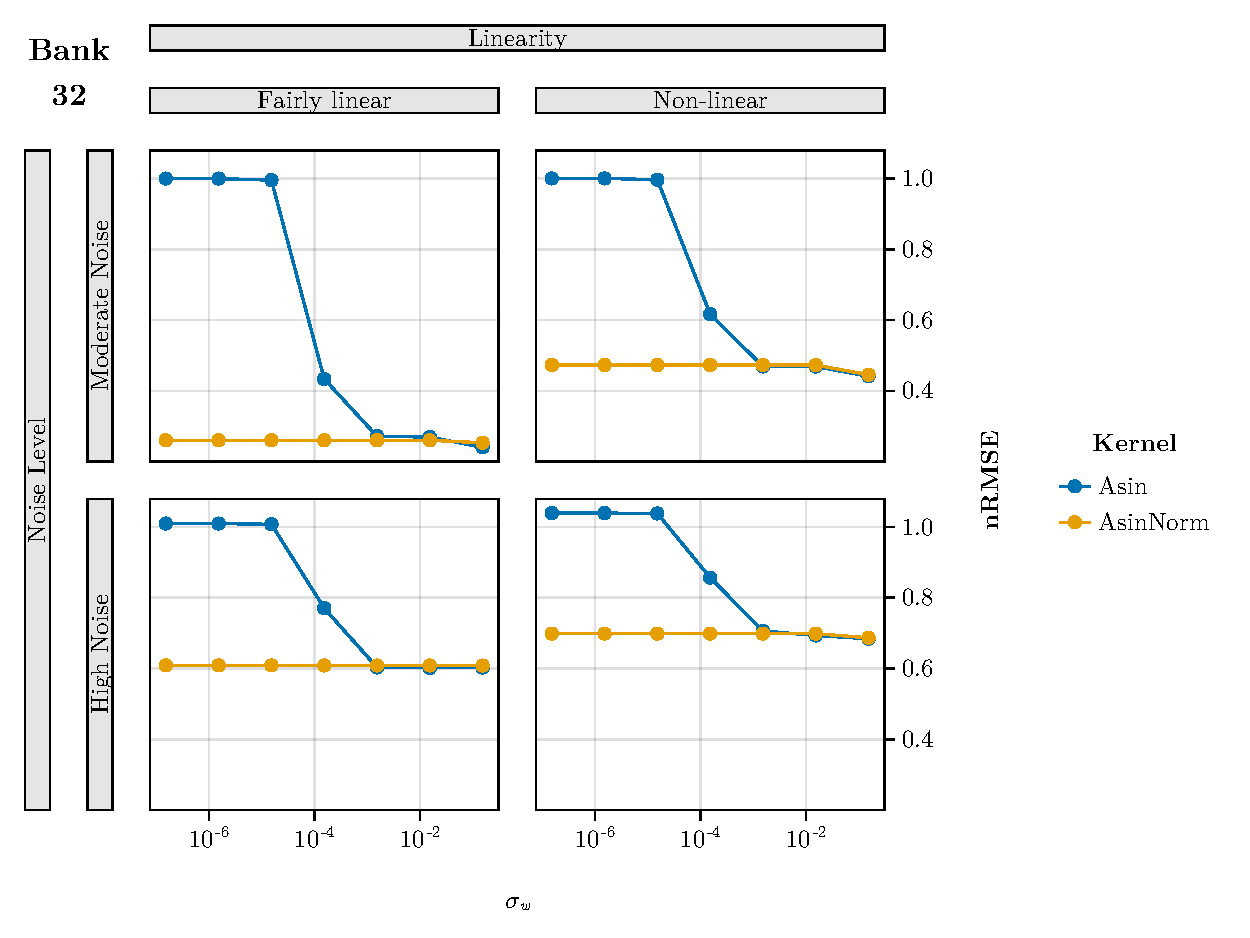
\includegraphics[width=0.7\textwidth]{plots/nRMSE_delve_bank_32_scaled}
    \caption{nRMSE results on Delve Bank32 dataset with $\sigma_w$ scaled}
    \label{fig:nrmse-delve-all-bank-32-scaled}
\end{figure}

\begin{figure}[H]
    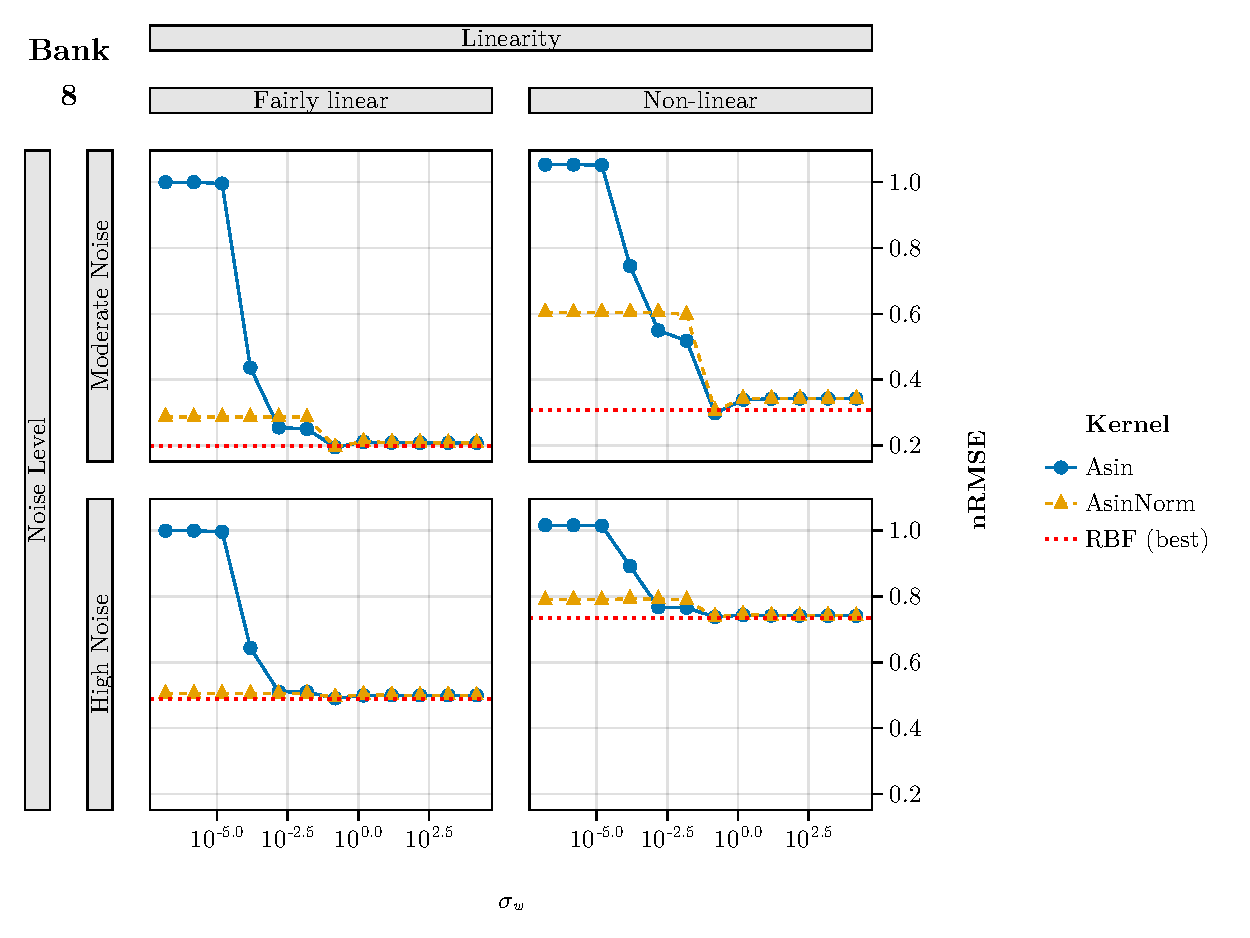
\includegraphics[width=0.7\textwidth]{plots/nRMSE_delve_bank_8_scaled}
    \caption{nRMSE results on Delve Bank8 dataset with $\sigma_w$ scaled}
    \label{fig:nrmse-delve-bank-8-scaled}
\end{figure}


\paragraph{Pumadyn Delve Dataset}

\begin{figure}[H]
    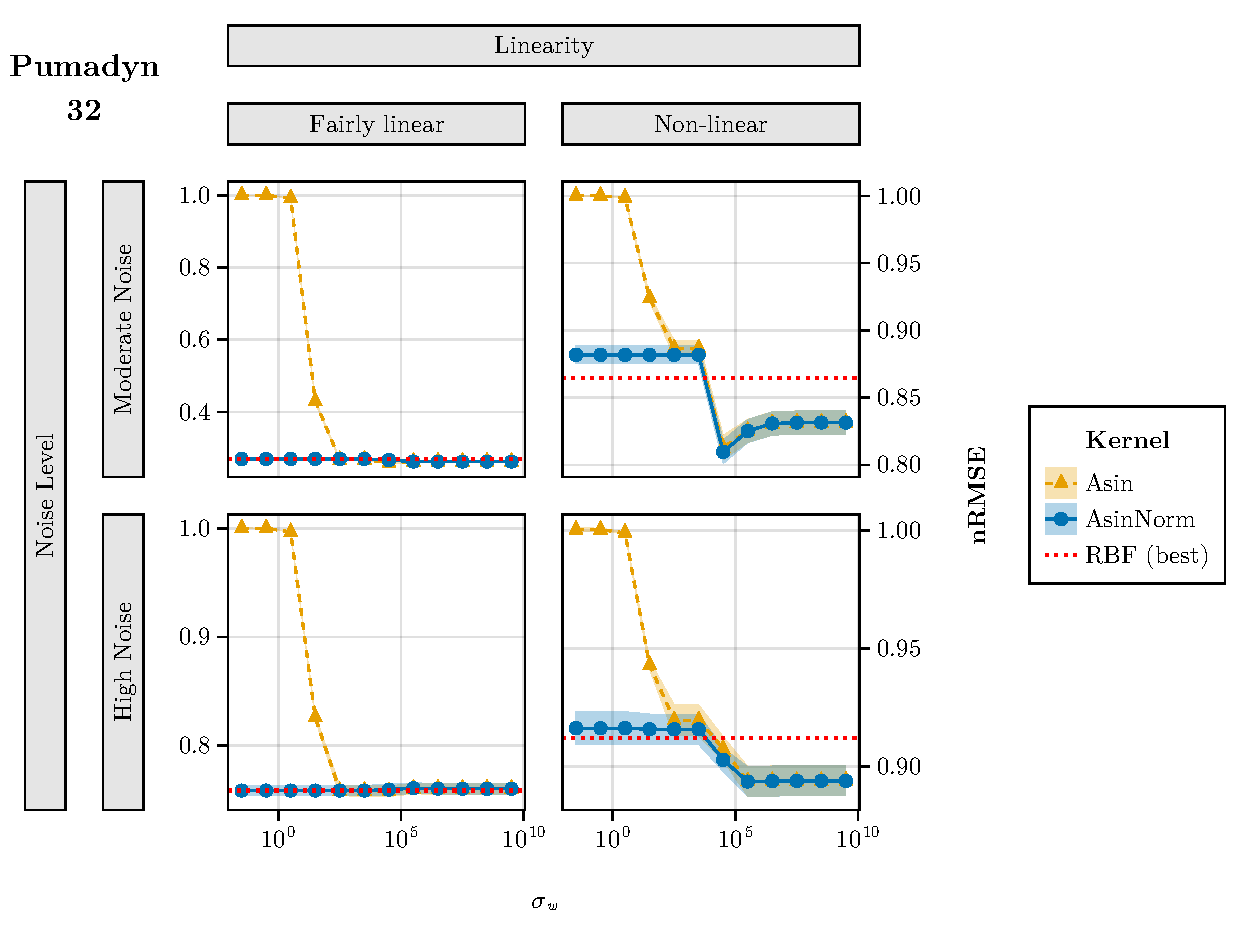
\includegraphics[width=0.7\textwidth]{plots/nRMSE_delve_pumadyn_32_scaled}
    \caption{nRMSE results on Delve PumaDyn32 dataset with $\sigma_w$ scaled}
    \label{fig:nrmse-delve-pumadyn-32-scaled}
\end{figure}

\begin{figure}[H]
    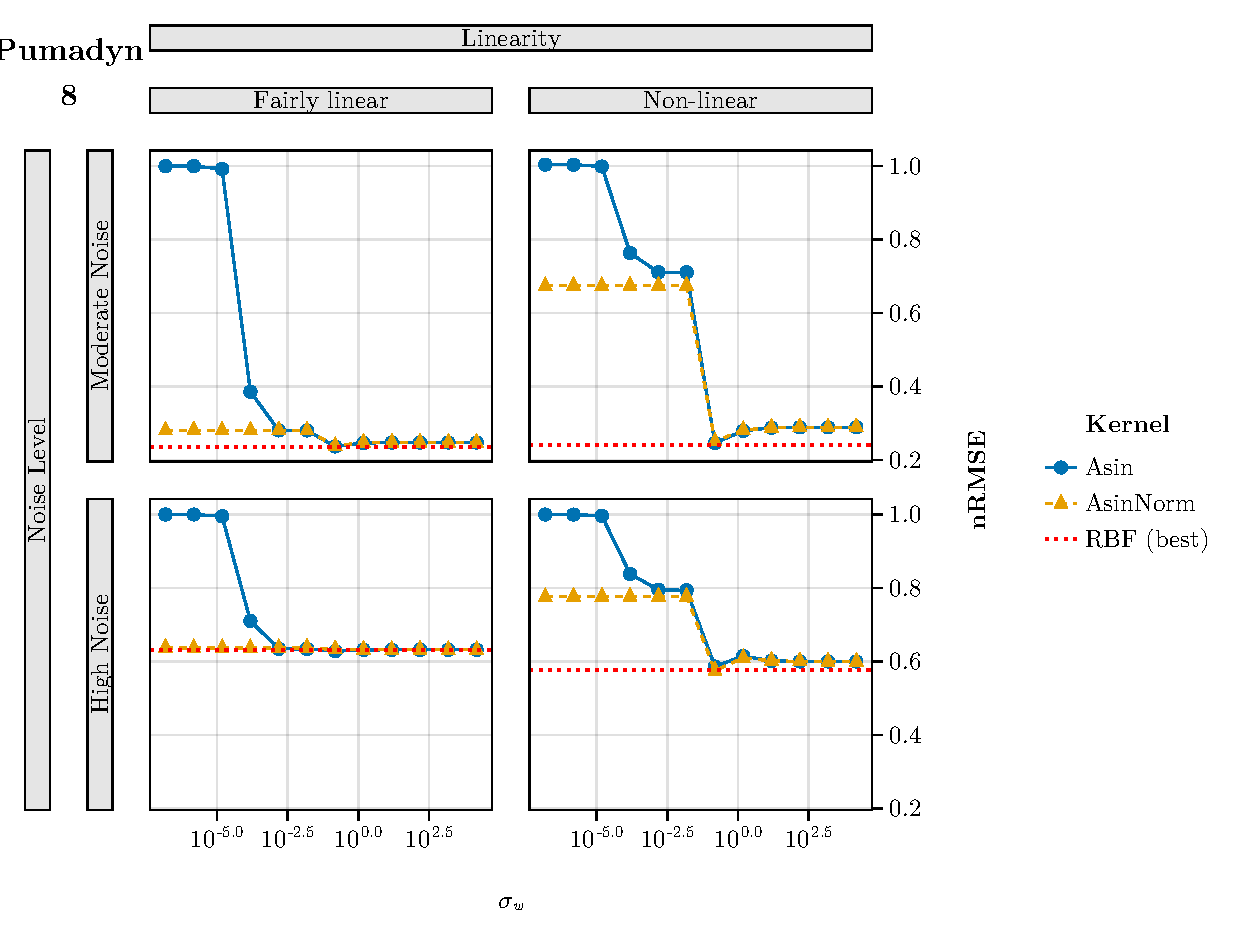
\includegraphics[width=0.7\textwidth]{plots/nRMSE_delve_pumadyn_8_scaled}
    \caption{nRMSE results on Delve PumaDyn8 dataset with $\sigma_w$ scaled}
    \label{fig:nrmse-delve-asinnorm-pumadyn-8-scaled}
\end{figure}

\subsubsection{Classification}

\begin{figure}[H]
    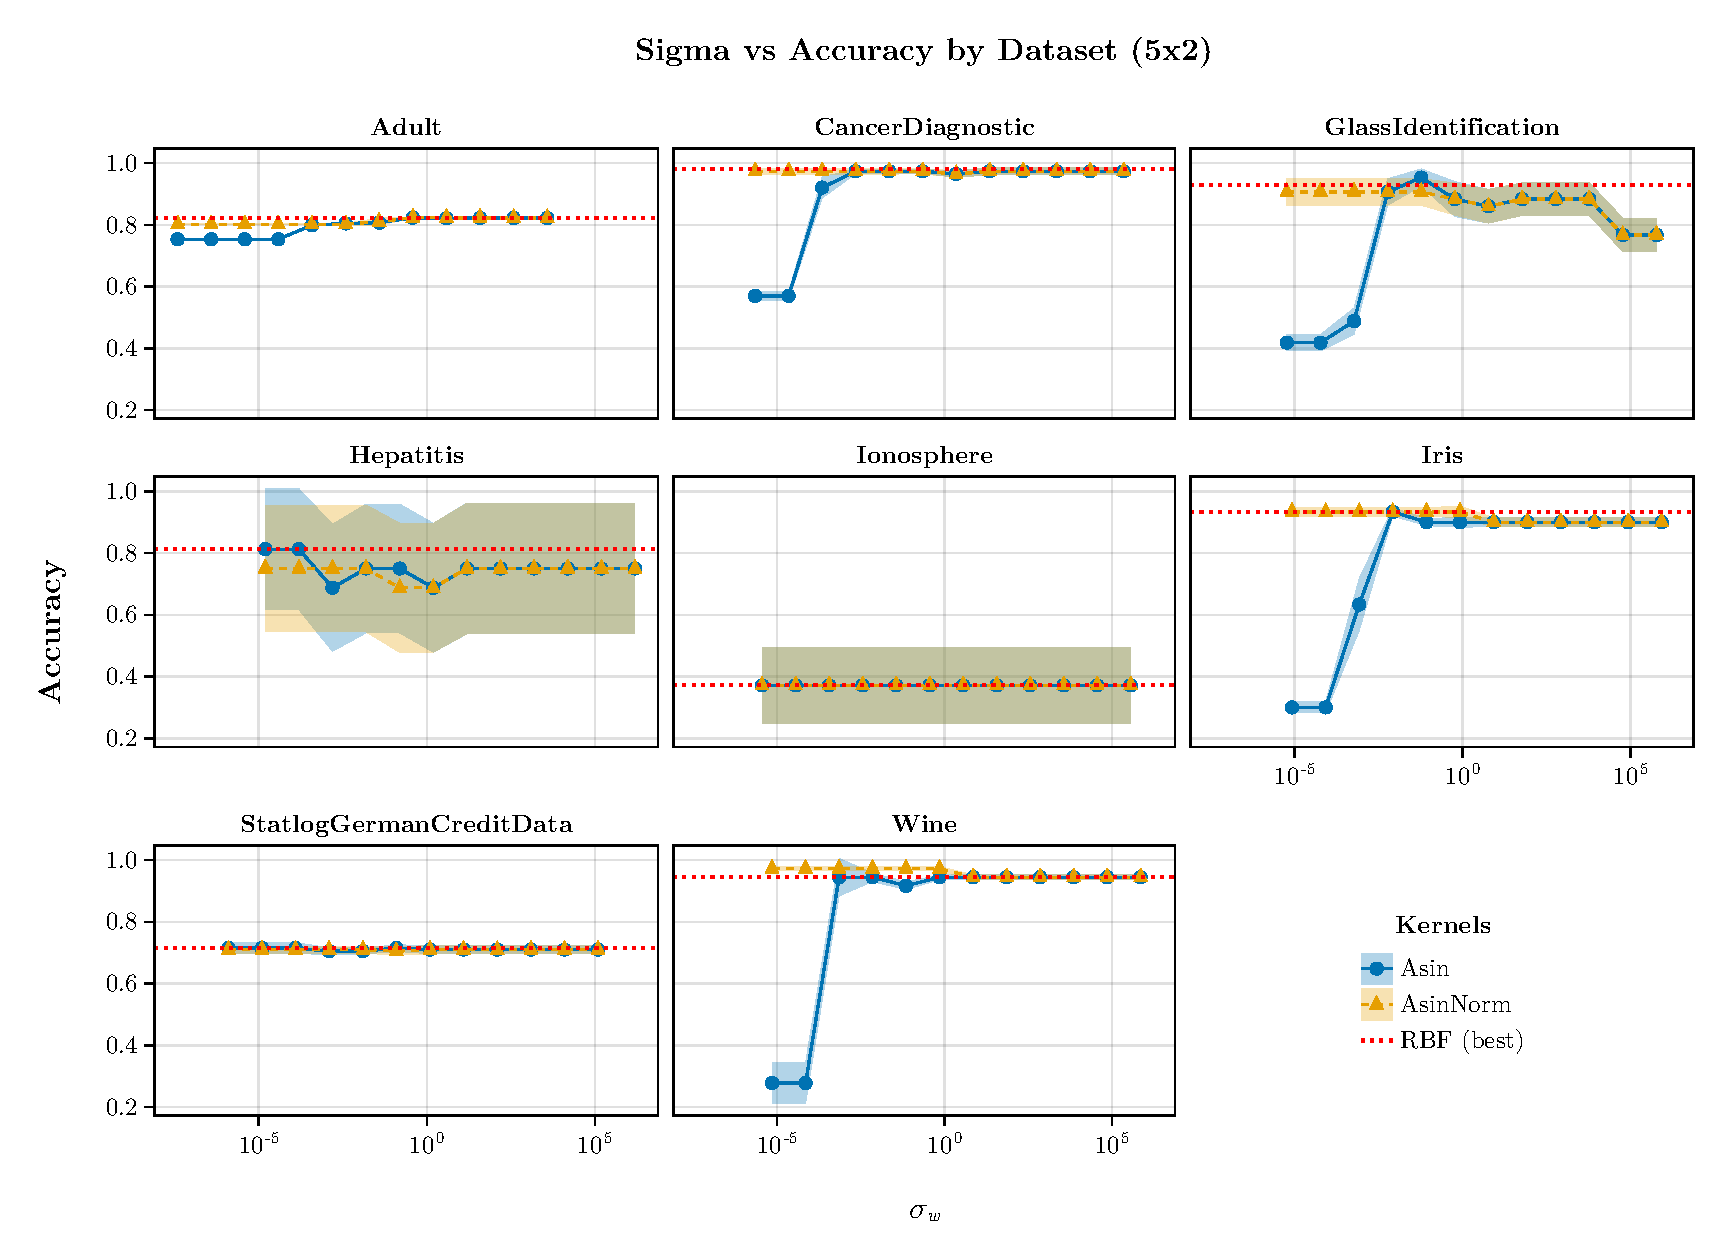
\includegraphics{plots/accuracy_class_all_scaled}
    \caption{Sigma vs Accuracy by dataset using Normalized arcsine kernel}%
    \label{fig:accuracy-asinnorm-scaled}
\end{figure}

\subsubsection{Comparison with radial basis (RBF) kernel}

\begin{figure}[H]
    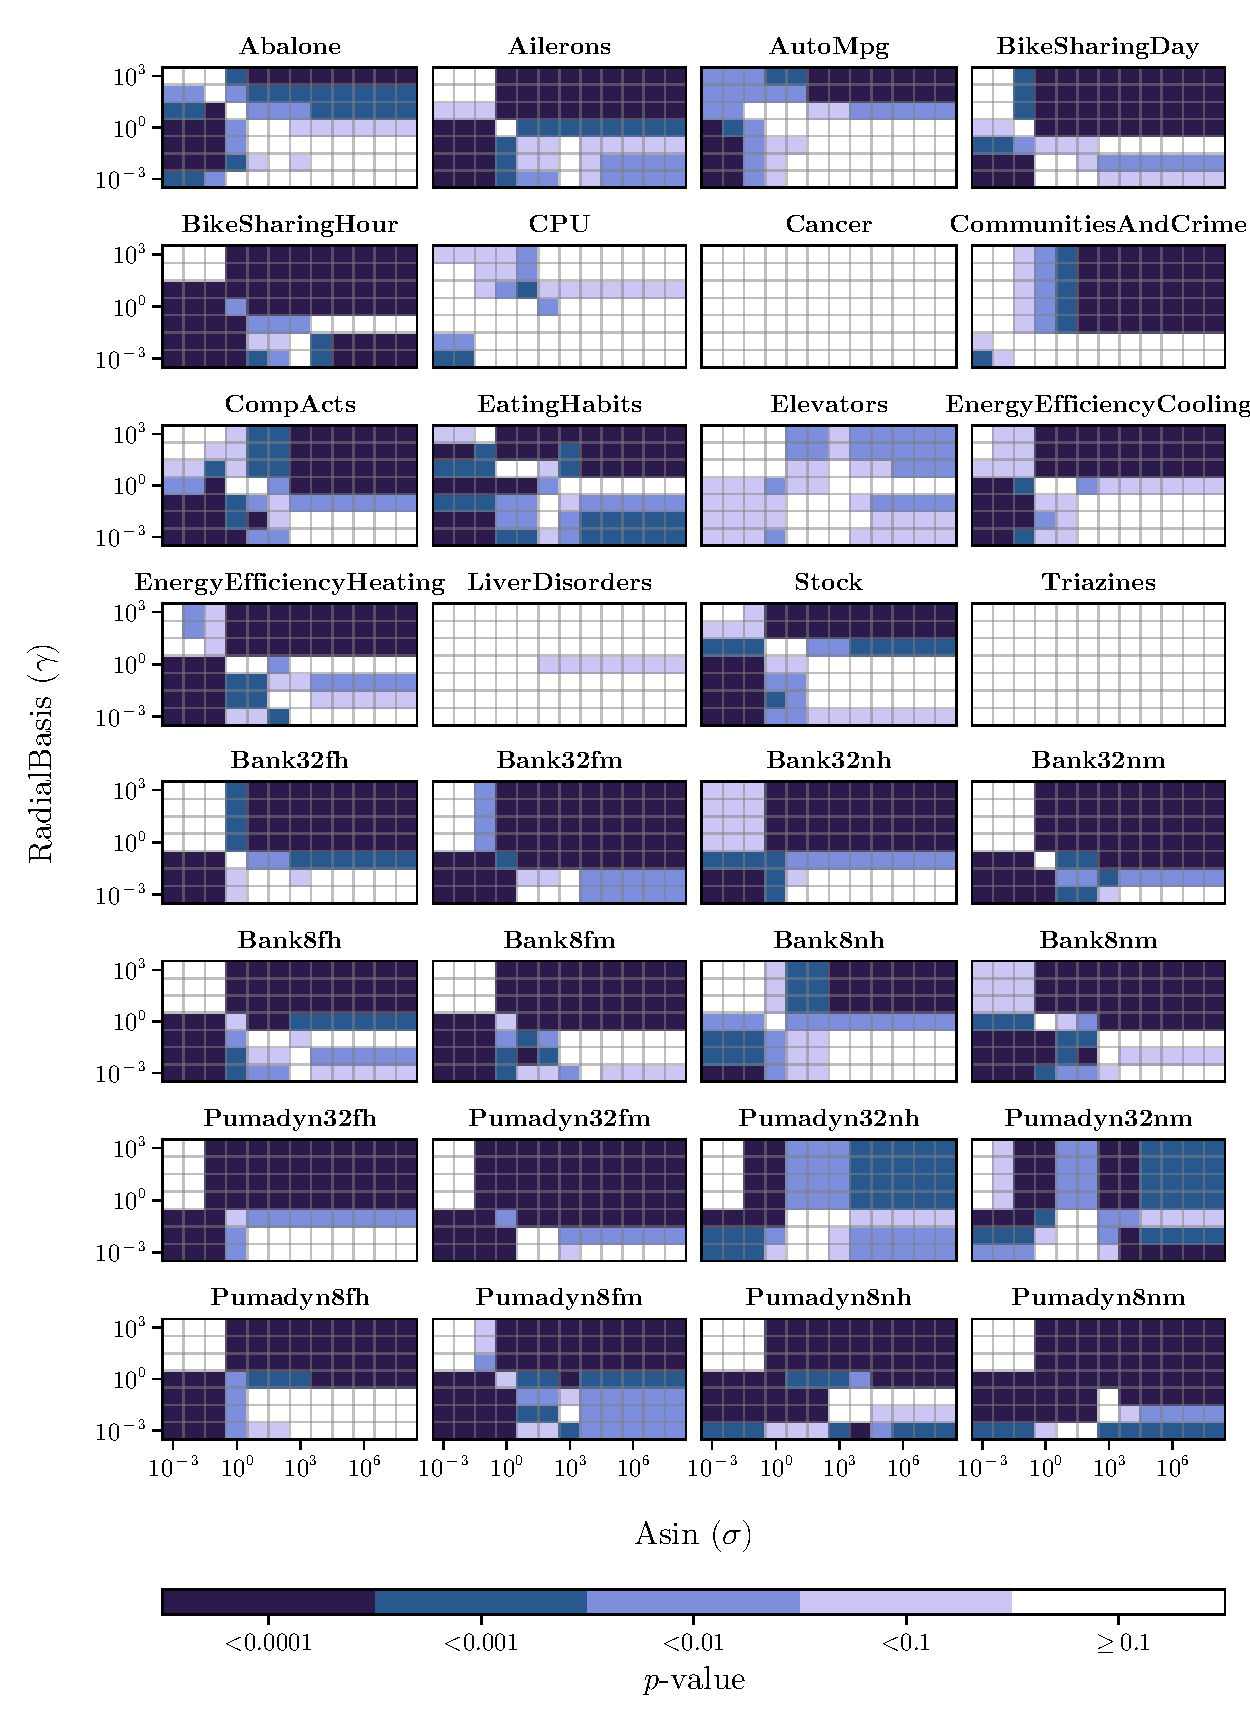
\includegraphics[width=0.9\textwidth]{plots/heatmaps_rbf_asin_pvalues}
    \caption{p values}
    \label{fig:paired-ttest-rbf-asinnorm}
\end{figure}

%  TODO: add pattern or something so the color can be seen in b/w
\begin{figure}[H]
    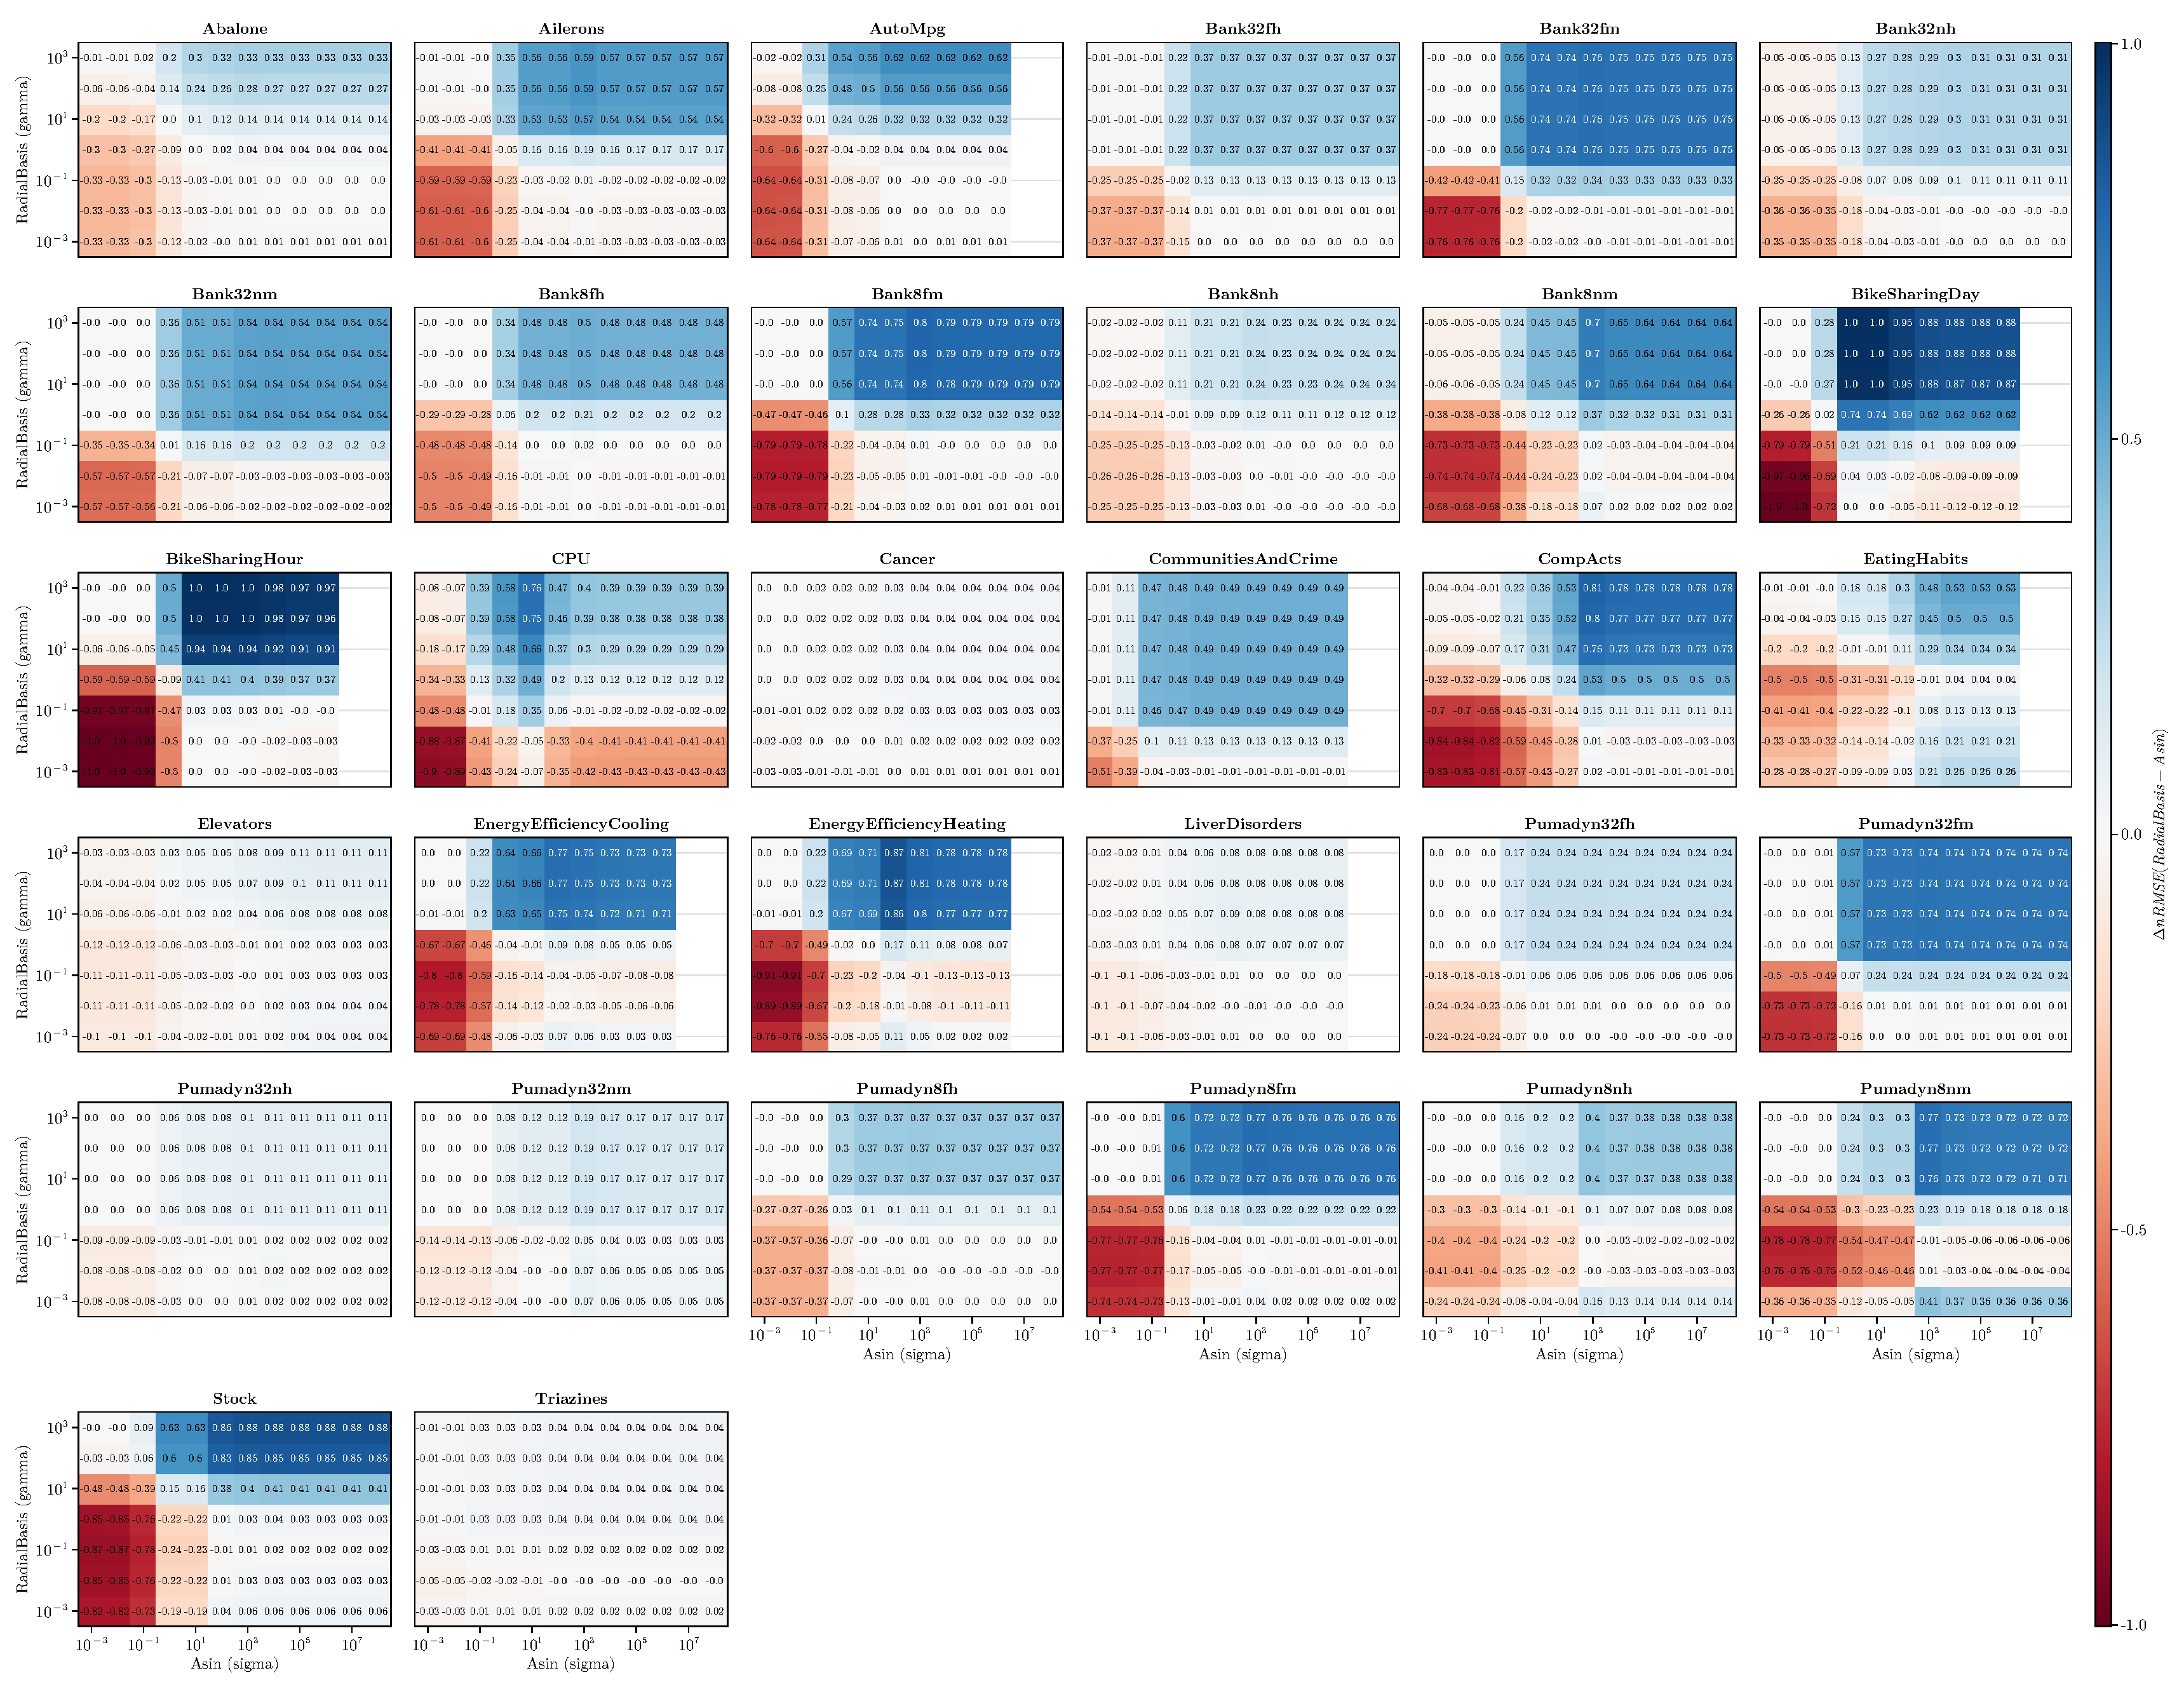
\includegraphics[width=0.9\textwidth]{plots/heatmaps_rbf_asin}
    \caption{Difference between nRMSE of RBF and normalized arc-sine kernels ($\alpha=0.001$)}
    \label{fig:paired-ttest-rbf-asinnorm-diff}
\end{figure}

\subsubsection{Computational Cost}


\pagebreak
\section{Arc-cosine kernels}
%! TEX root = **/000-main.tex
% vim: spell spelllang=en:


\subsection{Normalized arccosine kernels}

As explained in \cref{sub:kernel_normalization_acos}, the normalization of the
arccosine kernel makes the kernels insensitive to the scaling of the input data
proposed by \cite{pandeyGoDeepWide2014} as a way of introducing the $\sigma$
hyperparameter. This means that for the normalized arccosine kernel, there is
no $\sigma$ hyperparameter to tune. Additionally, for $n=0$, the kernel is
already normalized.

We can perform the paired t-test between the results obtained with each of the
normalized arccosine kernels and the radial basis kernel. Taking the best
performant hyperparamters (the ones that minimize the nRMSE) for each kernel and
dataset combination.

\subsubsection{Normalized Arccosine kernel for $n=0$}

\Cref{tab:paired_ttest_acos0_rbf} shows the results for the paired t-test of
the normalized arccosine kernel for $n=0$ against the radial basis kernel. Looking
at the $p$\textendash{}values, we can see that for most datasets, the null hypothesis
cannot be rejected, which means that we cannot reject the hypothesis that both
kernels perform the same. In bold, we highlight the $p$\textendash{}values that
reject the null hypothesis with a significance level of $\alpha = 0.001$. In all
these cases except for the \texttt{Pumadyn32nm} dataset, the RBF kernel performs
better than the normalized arccosine kernel for $n=0$.

\begin{table}[H]
    \caption{Results for the paired t-test of acos $n=0$ against RBF for regression datasets}
    \label{tab:paired_ttest_acos0_rbf}
    %! TEX root = **/000-main.tex
% vim: spell spelllang=en:
%
\begin{tabular}{lrrr}
	\toprule
	\textbf{DataSet}                          & \textbf{$p$\textendash{}value} & \textbf{$t$\textendash{}stat} & \textbf{$\Delta$nRMSE (RBF - Acos0)} \\\midrule
	Abalone                                   & 0.39                           & 0.95                          & 0.0014                               \\
	Ailerons                                  & \textbf{1.0e-5}                & 18.0                          & -0.12                                \\
	AutoMpg                                   & 0.32                           & 1.1                           & -0.034                               \\
	Bank32fh                                  & 0.25                           & -1.3                          & 0.0005                               \\
	Bank32fm                                  & \textbf{0.00016}               & 10.0                          & -0.019                               \\
	\addlinespace
	Bank32nh                                  & 0.054                          & 2.5                           & -0.013                               \\
	Bank32nm                                  & \textbf{1.2e-5}                & 17.0                          & -0.055                               \\
	Bank8fh                                   & \textbf{0.00011}               & 11.0                          & -0.03                                \\
	Bank8fm                                   & \textbf{2.7e-5}                & 15.0                          & -0.065                               \\
	Bank8nh                                   & \textbf{0.00042}               & 8.3                           & -0.04                                \\
	\addlinespace
	Bank8nm                                   & \textbf{4.0e-6}                & 21.0                          & -0.23                                \\
	% BikeSharingDay          & \textbf{1.8e-9}                & 100.0                         & -1.0                                 \\
	% BikeSharingHour         & \textbf{2.4e-9}                & 96.0                          & -1.9                                 \\
	CPU                                       & 0.034                          & 2.9                           & -0.54                                \\
	Cancer                                    & 0.47                           & 0.78                          & 0.01                                 \\
	CommunitiesAndCrime                       & 0.0015                         & 6.3                           & -0.6                                 \\
	CompActs                                  & 0.088                          & 2.1                           & -0.051                               \\
	\addlinespace
	EatingHabits                              & 0.0015                         & 6.3                           & -0.68                                \\
	Elevators                                 & 0.17                           & 1.6                           & 0.0023                               \\
	% EnergyEfficiencyCooling & \textbf{3.1e-5}                & 14.0                          & -0.91                                \\
	% EnergyEfficiencyHeating & \textbf{7.8e-8}                & 48.0                          & -0.94                                \\
	% LiverDisorders       & 0.29                           & 1.2                           & -1.1                                 \\
	Pumadyn32fh                               & 0.74                           & 0.35                          & -0.00074                             \\
	Pumadyn32fm                               & 0.1                            & -2.0                          & 0.0064                               \\
	Pumadyn32nh                               & 0.0037                         & -5.1                          & 0.021                                \\
	\addlinespace
	\rowcolor[gray]{0.85}\textbf{Pumadyn32nm} & \textbf{0.00058}               & -7.7                          & \textbf{0.038}                       \\
	Pumadyn8fh                                & 0.031                          & 3.0                           & -0.0079                              \\
	Pumadyn8fm                                & \textbf{4.5e-5}                & 13.0                          & -0.037                               \\
	Pumadyn8nh                                & \textbf{0.00022}               & 9.5                           & -0.068                               \\
	Pumadyn8nm                                & \textbf{4.2e-8}                & 54.0                          & -0.16                                \\
	\addlinespace
	Stock                                     & 0.41                           & -0.9                          & 0.0048                               \\
	Triazines                                 & 0.96                           & 0.058                         & -0.0064                              \\\bottomrule
\end{tabular}

\end{table}

\subsubsection{Normalized Arccosine kernel for $n=1$}

\cref{tab:paired_ttest_acos1_rbf} shows the results for the paired t-test of
the normalized arccosine kernel for $n=1$ against the radial basis kernel in the
same format as \cref{tab:paired_ttest_acos0_rbf}. In this case, there are no
datasets where the arccosine kernel outperforms the RBF kernel in a statistically
significant way. Comparing the $p$\textendash{}values with the ones obtained
in \cref{tab:paired_ttest_acos0_rbf}, we can see that they are in the same order
of magnitude for most datasets. In fact, the datasets in which the $p$\textendash{}values
reject the null hypothesis are the same, except for the \texttt{Pumadyn32nm}, which
for $n=1$ the null hypothesis cannot be rejected.

\begin{table}[H]
    \caption{Results for the paired t-test of acos $n=1$ against RBF for regression datasets}
    \label{tab:paired_ttest_acos1_rbf}
    %! TEX root = **/000-main.tex
% vim: spell spelllang=en:
%
\begin{tabular}{lrrr}
	\toprule
	\textbf{DataSet}    & \textbf{$p$\textendash{}value} & \textbf{$t$\textendash{}stat} & \textbf{$\Delta$nRMSE (RBF - Acos1)} \\\midrule
	Abalone             & 0.5                            & -0.73                         & 0.0088                               \\
	Ailerons            & \textbf{0.00025}               & 9.2                           & -0.065                               \\
	AutoMpg             & 0.13                           & 1.8                           & -0.029                               \\
	Bank32fh            & 0.18                           & 1.5                           & -0.0082                              \\
	Bank32fm            & \textbf{0.00011}               & 11.0                          & -0.009                               \\
	\addlinespace
	Bank32nh            & 0.02                           & 3.4                           & -0.0048                              \\
	Bank32nm            & \textbf{0.0003}                & 8.9                           & -0.015                               \\
	Bank8fh             & \textbf{0.00074}               & 7.3                           & -0.022                               \\
	Bank8fm             & \textbf{0.00016}               & 10.0                          & -0.05                                \\
	Bank8nh             & \textbf{0.0003}                & 8.9                           & -0.025                               \\
	\addlinespace
	Bank8nm             & \textbf{2.7e-5}                & 15.0                          & -0.17                                \\
	% BikeSharingDay                                                & 0.00026          & 9.1              & -0.11            \\
	% BikeSharingHour                                               & 5.6e-6           & 20.0             & -0.029           \\
	CPU                 & 0.17                           & 1.6                           & -0.49                                \\
	Cancer              & 0.14                           & 1.7                           & -0.0035                              \\
	CommunitiesAndCrime & 0.85                           & 0.21                          & -0.014                               \\
	CompActs            & 0.59                           & 0.58                          & -0.025                               \\
	\addlinespace
	EatingHabits        & 0.092                          & 2.1                           & -0.02                                \\
	Elevators           & 0.16                           & 1.7                           & -0.0091                              \\
	% EnergyEfficiencyCooling                                       & 0.15             & 1.7              & -0.044           \\
	% EnergyEfficiencyHeating                                       & 0.00011          & 11.0             & -0.078           \\
	% LiverDisorders                                                & 0.39             & 0.93             & -0.019           \\
	Pumadyn32fh         & 0.055                          & 2.5                           & -0.0054                              \\
	Pumadyn32fm         & 0.11                           & 2.0                           & -0.0083                              \\
	Pumadyn32nh         & 0.38                           & -0.97                         & -0.0028                              \\
	\addlinespace
	Pumadyn32nm         & 0.035                          & 2.9                           & -0.014                               \\
	Pumadyn8fh          & 0.0067                         & 4.5                           & -0.0092                              \\
	Pumadyn8fm          & \textbf{1.8e-6}                & 25.0                          & -0.057                               \\
	Pumadyn8nh          & \textbf{2.6e-6}                & 23.0                          & -0.17                                \\
	Pumadyn8nm          & \textbf{1.6e-7}                & 41.0                          & -0.42                                \\
	\addlinespace
	Stock               & 0.55                           & 0.64                          & 0.0047                               \\
	Triazines           & 0.75                           & -0.34                         & -0.0018                              \\\bottomrule
\end{tabular}

\end{table}

\subsubsection{Normalized Arccosine kernel for $n=2$}

\Cref{tab:paired_ttest_acos2_rbf} shows the results for the paired t-test of
the normalized arccosine kernel for $n=2$ against the radial basis kernel in the
same format as \cref{tab:paired_ttest_acos0_rbf}. The results in terms of
the significance level of the $p$\textendash{}values are similar to the ones
when $n=1$. The only differences are \texttt{Pumadyn8fh} and \texttt{Pumadyn8nh}.
% which for $n=1$ % TODO: finish sentence !!!!

\begin{table}[H]
    \caption{Results for the paired t-test of acos $n=2$ against RBF for regression datasets}
    \label{tab:paired_ttest_acos2_rbf}
    %! TEX root = **/000-main.tex
% vim: spell spelllang=en:
%
\begin{tabular}{lrrr}
	\toprule
	\textbf{DataSet}    & \textbf{$p$\textendash{}value} & \textbf{$t$\textendash{}stat} & \textbf{$\Delta$nRMSE (RBF - Acos2)} \\\midrule
	Abalone             & 0.34                           & -1.1                          & 0.0074                               \\
	Ailerons            & \textbf{0.00027}               & 9.1                           & -0.06                                \\
	AutoMpg             & 0.81                           & 0.26                          & -0.009                               \\
	Bank32fh            & 0.54                           & 0.65                          & -0.0062                              \\
	Bank32fm            & \textbf{0.0002}                & 9.7                           & -0.0094                              \\
	\addlinespace
	Bank32nh            & 0.0036                         & 5.1                           & -0.0044                              \\
	Bank32nm            & \textbf{0.00036}               & 8.5                           & -0.012                               \\
	Bank8fh             & \textbf{0.0006}                & 7.7                           & -0.022                               \\
	Bank8fm             & \textbf{0.00016}               & 10.0                          & -0.041                               \\
	Bank8nh             & 0.0024                         & 5.7                           & -0.021                               \\
	\addlinespace
	Bank8nm             & \textbf{5.5e-5}                & 13.0                          & -0.13                                \\
	% BikeSharingDay & 0.001 & 6.8 & -0.088 \\
	% BikeSharingHour & 9.8e-6 & 18.0 & -0.028 \\
	CPU                 & 0.31                           & 1.1                           & -0.47                                \\
	Cancer              & 0.45                           & 0.81                          & -0.0038                              \\
	CommunitiesAndCrime & 0.99                           & 0.011                         & -0.0087                              \\
	CompActs            & 0.56                           & 0.63                          & -0.029                               \\
	\addlinespace
	EatingHabits        & 0.13                           & 1.8                           & -0.037                               \\
	Elevators           & 0.15                           & 1.7                           & -0.0045                              \\
	% EnergyEfficiencyCooling & 0.46 & 0.81 & -0.027 \\
	% EnergyEfficiencyHeating & 0.009 & 4.1 & -0.035 \\
	% LiverDisorders & 0.26 & 1.3 & -0.016 \\
	Pumadyn32fh         & 0.015                          & 3.6                           & -0.0099                              \\
	Pumadyn32fm         & 0.05                           & 2.6                           & -0.0087                              \\
	Pumadyn32nh         & 0.54                           & 0.66                          & -0.0076                              \\
	\addlinespace
	Pumadyn32nm         & 0.0047                         & 4.8                           & -0.02                                \\
	Pumadyn8fh          & \textbf{2.4e-5}                & 15.0                          & -0.0068                              \\
	Pumadyn8fm          & \textbf{0.00017}               & 10.0                          & -0.028                               \\
	Pumadyn8nh          & 0.0069                         & 4.4                           & -0.03                                \\
	Pumadyn8nm          & \textbf{8.2e-6}                & 19.0                          & -0.11                                \\
	\addlinespace
	Stock               & 0.71                           & 0.39                          & -0.0086                              \\
	Triazines           & 0.9                            & 0.14                          & -0.014                               \\\bottomrule
\end{tabular}

\end{table}

\subsection{Non-Normalized arccosine kernels}

As explained above, for the case of $n=0$, the arccosine kernel is already
normalized, so we only need to consider the cases where $n=1$ and $n=2$.

When running the experiments with the non-normalized versions of the arc-cosine
kernels, the execution time was significantly higher than the normalized versions.
With higher values of the cost ($C$) parameter, the execution time when $n=2$ was
extremely high for larger datasets, and the SMO algorithm that \libsvm uses to find
the support vectors reached the maximum number of iterations without converging.


\begin{figure}[H]
    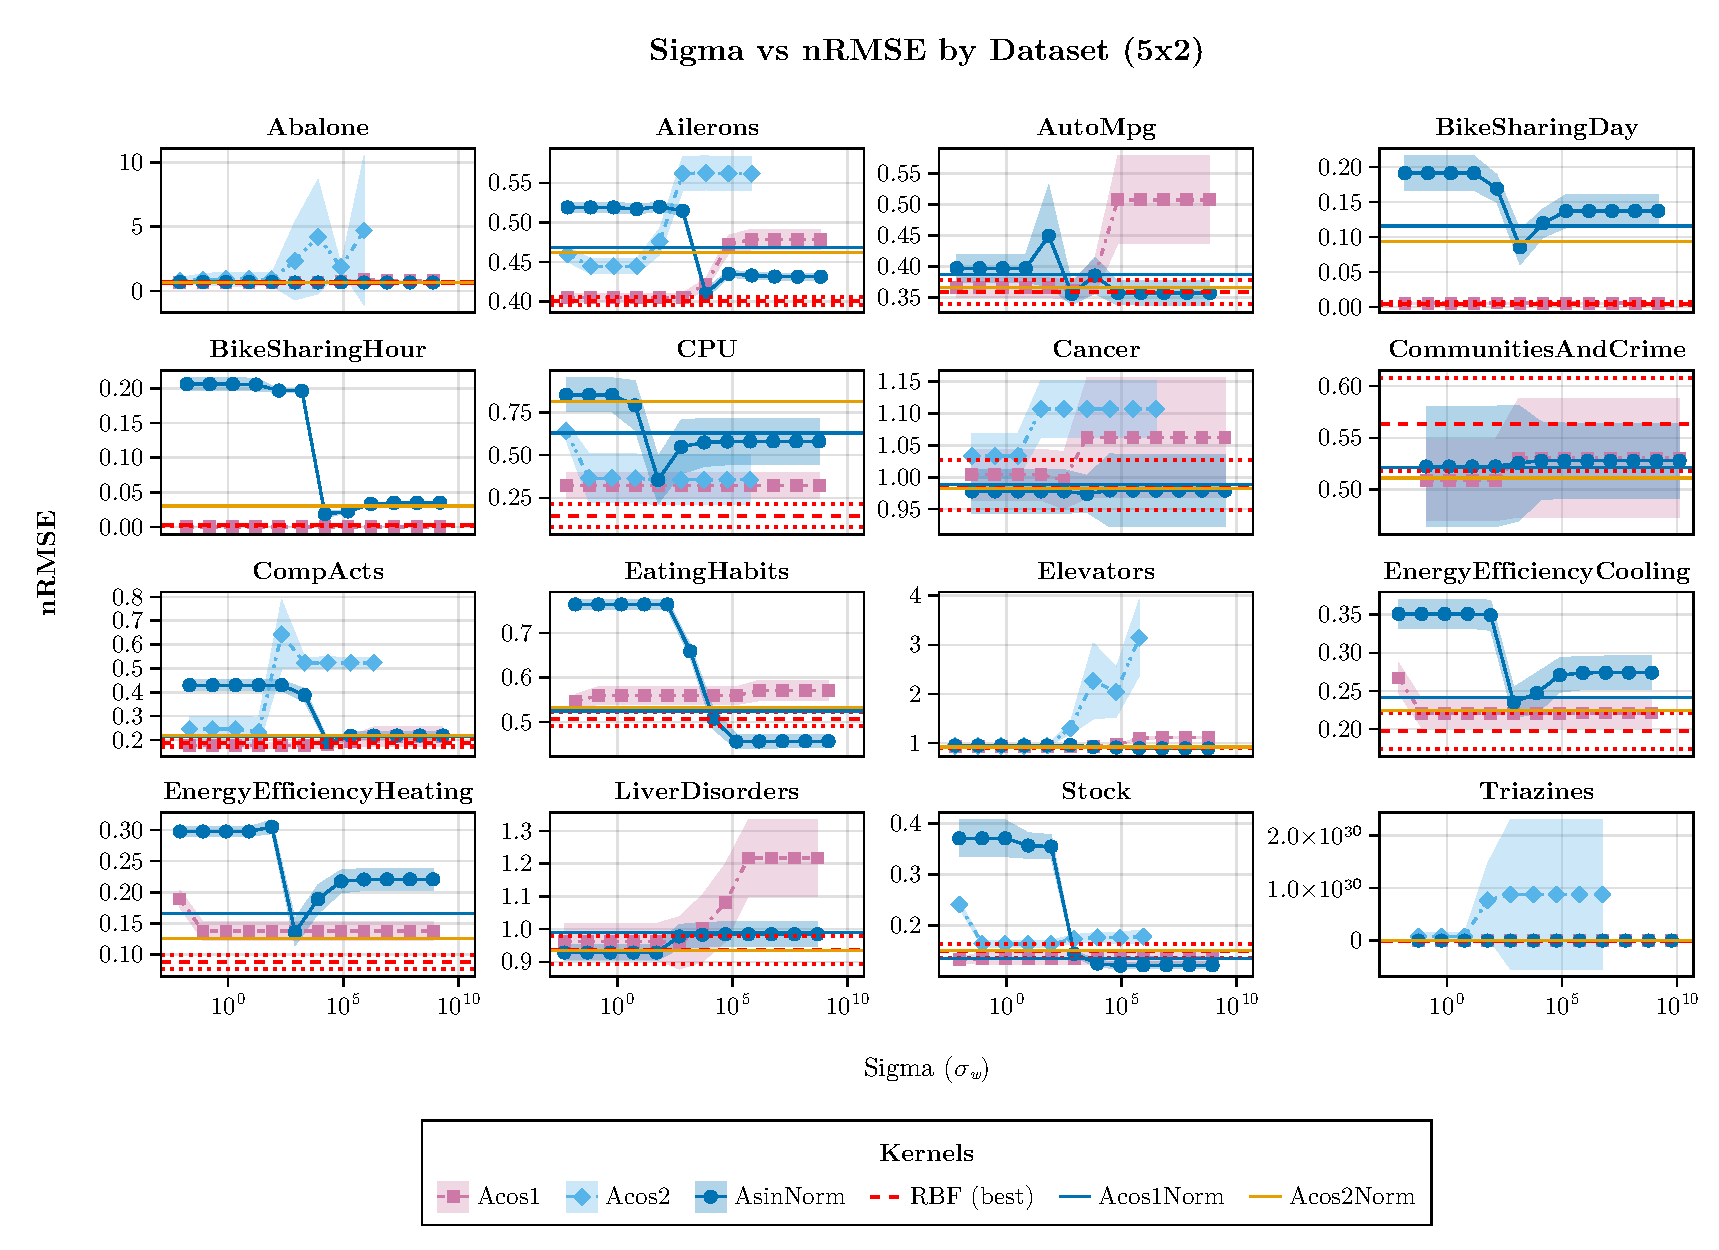
\includegraphics[width=\textwidth]{plots/nRMSE_nodelve_acos_scaled}
\end{figure}

\subsubsection{Arccosine kernel for $n=1$}

\subsubsection{Arccosine kernel for $n=2$}


% %! TEX root = **/000-main.tex
% vim: spell spelllang=en:


% \begin{figure}[H]
%     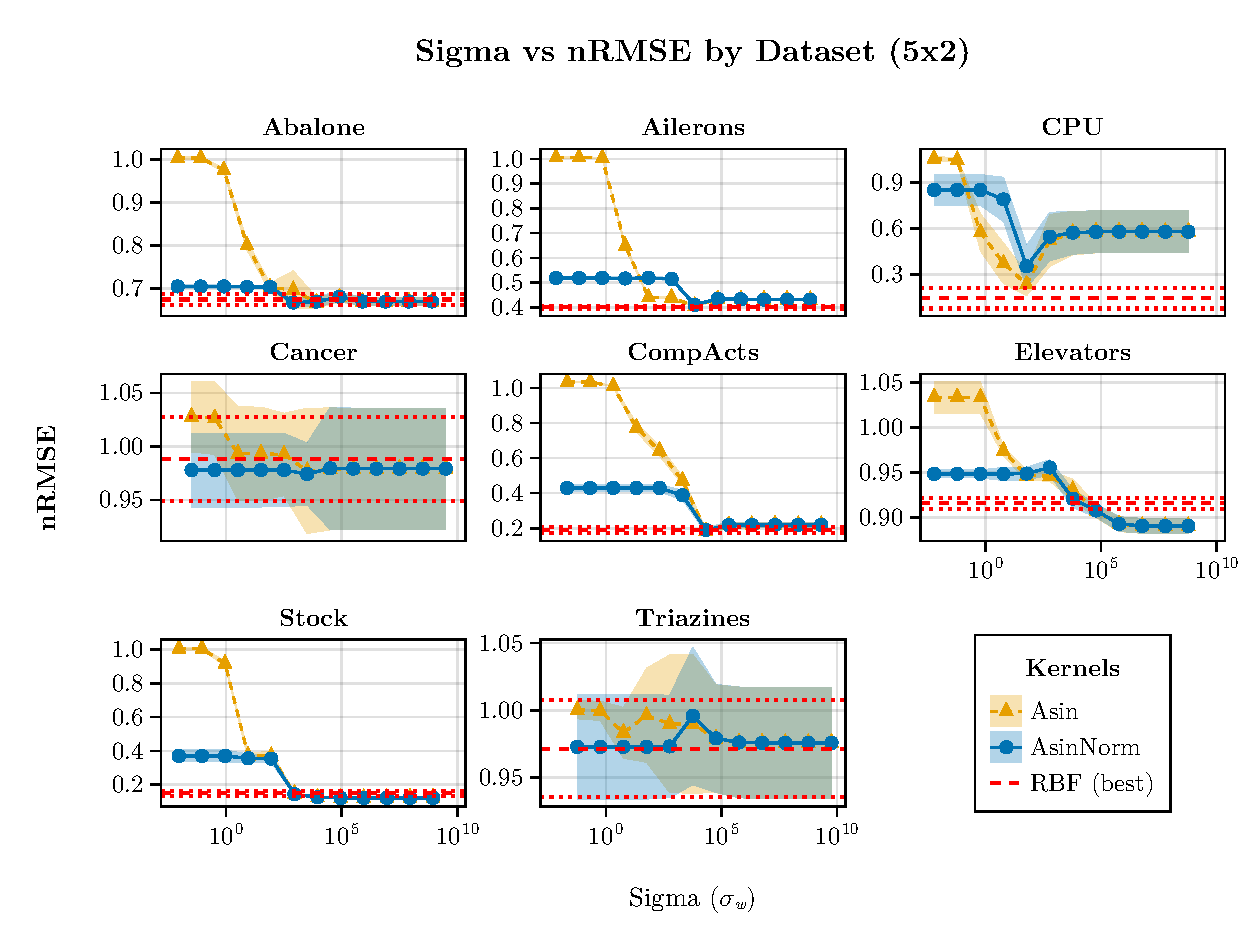
\includegraphics{plots/nRMSE_frenay_scaled}
%     \caption{nRMSE results on datasets from \cite{frenayParameterinsensitiveKernelExtreme2011} with
%         scaled $\sigma_w$}%
%     \label{fig:nrmse-frenay-scaled}
% \end{figure}
%
% \Cref{fig:nrmse-frenay-scaled} shows the results of the arc-sine kernel using
% \emph{nRMSE} as the performance measure and with $\sigma_w$ scaled. These allow
% us to compare the results between datasets.
%
% \begin{cnote}
%     Add copy of the table of Frénay and Verleysen along with the equivalent
%     table for our results?
%
%     The table is quite dense, so putting them side by side may be too much.
%
%     Figure out what is the most relevant information to show, rest in the
%     appendix
% \end{cnote}
%
% \subsection{Results for the arc cosine kernel on the Frenay datasets}
%
% \Cref{fig:nrmse-acos-frenay-scaled} shows the results when using the arc cosine kernels
% with $n=0,1,2$ on the Frenay datasets.
%
% \begin{figure}[H]
%     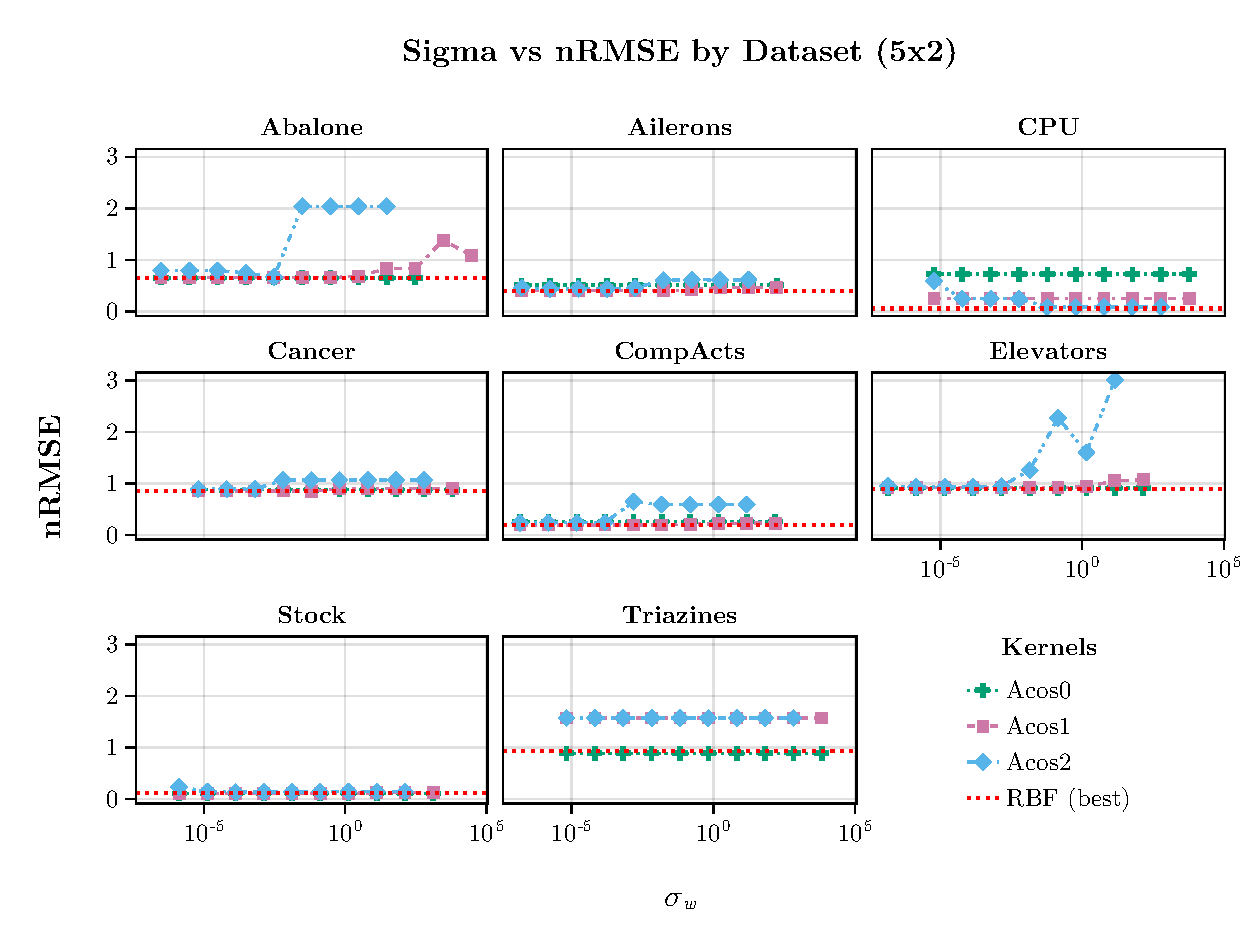
\includegraphics{plots/nRMSE_acos_frenay_scaled}
%     \caption{nRMSE results on datasets from \cite{frenayParameterinsensitiveKernelExtreme2011} with
%         scaled $\sigma_w$ using Arc cosine kernel}%
%     \label{fig:nrmse-acos-frenay-scaled}
% \end{figure}
% % FIX: std of Triazines goes crazy with acos2
%
% \begin{cnote}
%     Arc cosine kernel for n=2 is too slow (specially when $cost>1000$)
%     I have removed it, but ideally we run it with a smaller parameter grid.
%     Should be addressed either way.
% \end{cnote}
%
% % TODO: no em convenc el titol
% \section{Paired t-test results}
%
% Although the previous results are interesting, they are not conclusive and
% are based merely on the visual inspection of the plots. In order to draw
% conclusions, we need to perform a statistical test to see if there is
% really any meaningful difference between the models.
%
% As explained in \cref{sec:paired-t-test}, we will use the 5\texttimes2
% paired $t$-test. With this test, the null hypothesis is that the two models
% have equal performance.
%
% \subsection{RBF vs Arc-sine}
%
% We start by comparing the RBF kernel with the normalized arc-sine kernel for
% different values of $\sigma_w$ and $\gamma$ using $nRMSE$ as the performance
% measure. The results are shown in \cref{fig:paired-ttest-rbf-asinnorm},
% which shows the matrix of $p$-values shaded by the significance level,
% darker the color, the more significant the difference between the two models.
%
% % TODO: is this the most sensible way or should we approach it differently?
% The values of $\epsilon$ and $C$ are selected as the ones which obtained
% the performed best for each $\sigma$ and $\gamma$.
%
% \begin{figure}[H]
%     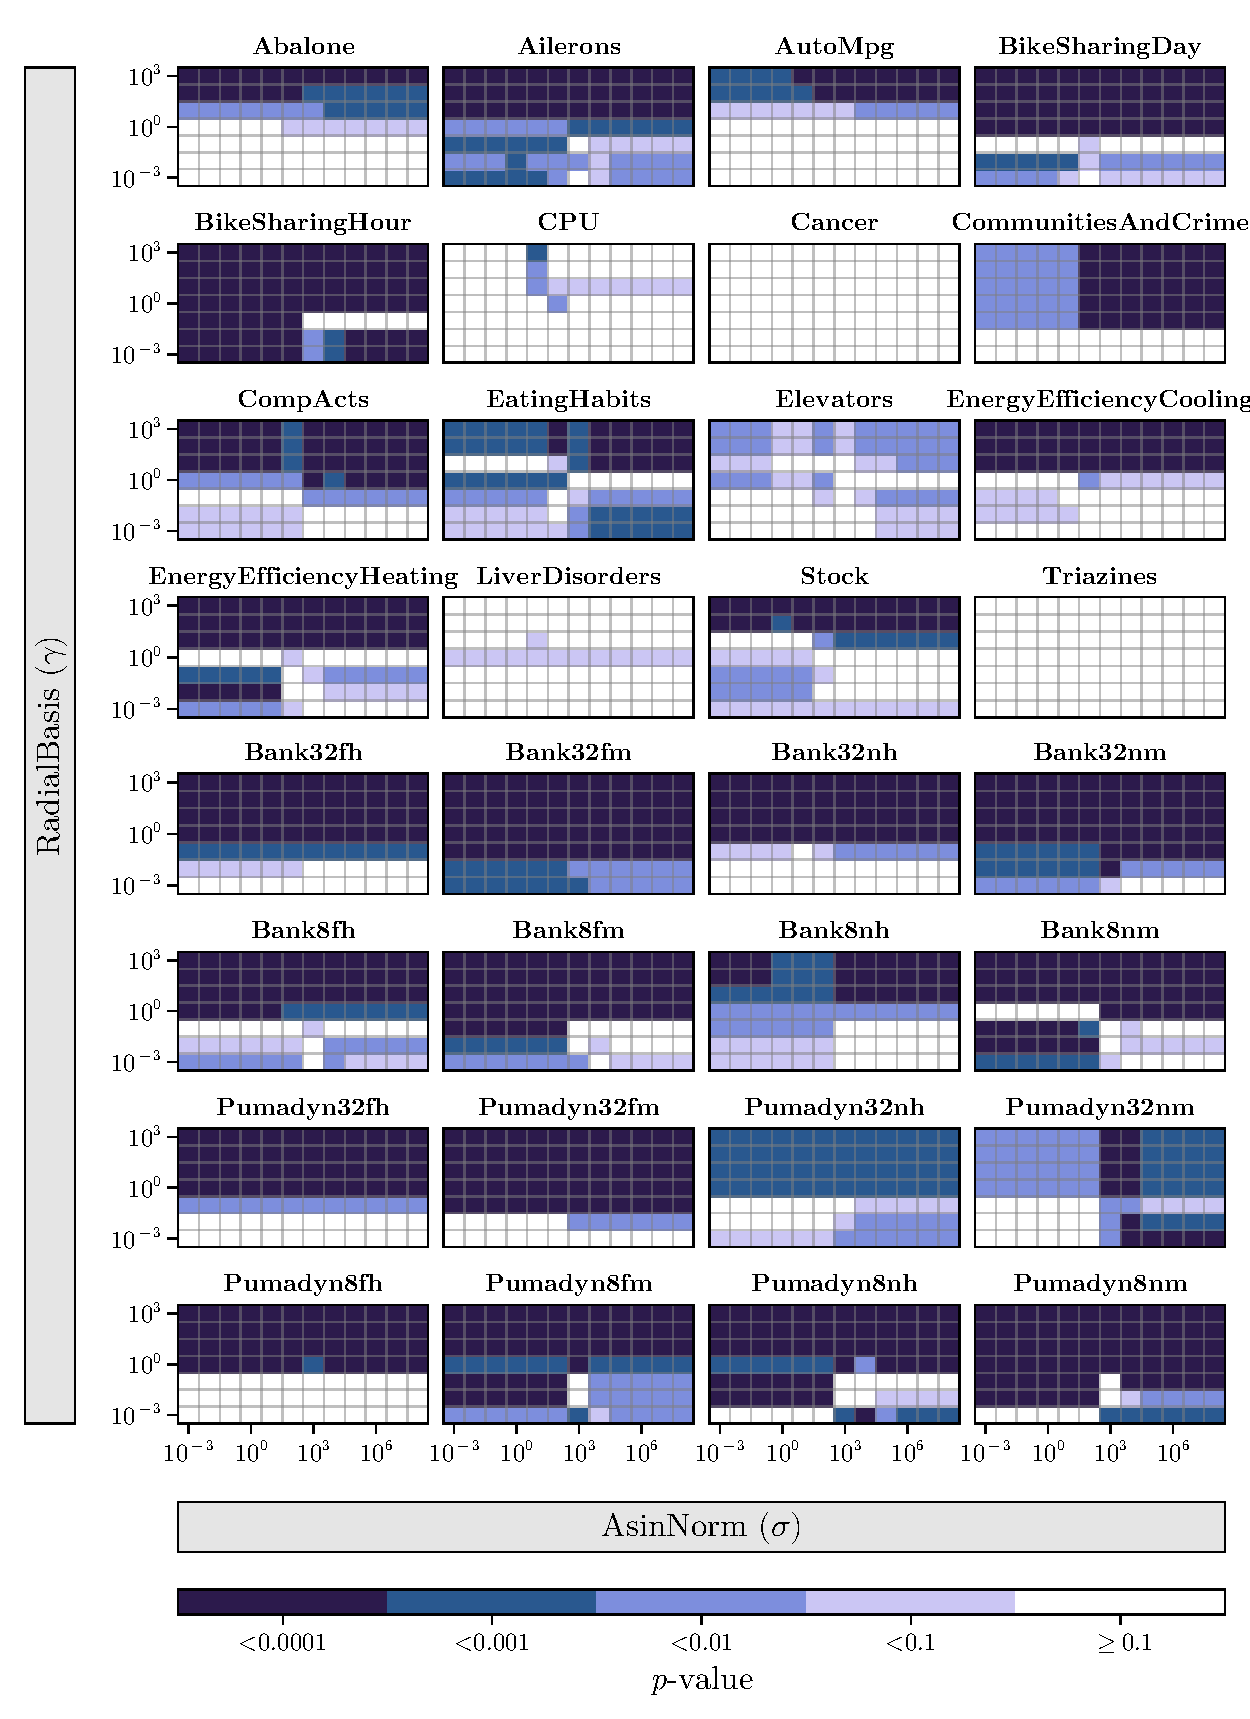
\includegraphics[width=0.9\textwidth]{plots/heatmaps_rbf_asinnorm_pvalues}
%     \caption{p values}
%     \label{fig:paired-ttest-rbf-asinnorm}
% \end{figure}
%
% In \cref{fig:paired-ttest-rbf-asinnorm}, we can see that for datasets
% \texttt{Cancer} and \texttt{Triazines}, there is no pair of hyperparameter
% values for which the difference between the two models is significant even at
% $\alpha=0.1$. For \texttt{LiverDisorders} and \texttt{Elevators}, the significance
% level is not below $\alpha=0.01$ for any pair of hyperparameters.
%
% The matrices shown in \cref{fig:paired-ttest-rbf-asinnorm} show which are the
% pairs which are statistically different, but do not show the magnitude or
% direction of the difference. For that, we can take the mean values of
% the difference in $NRMSE$ between the two models for each pair of hyperparameters
% and plot them as shown in \cref{fig:paired-ttest-rbf-asinnorm-diff}.
%
% The plot illustrates the difference between the RBF and normalized arc-sine
% kernels. Positive values indicate that the RBF had a higher $NRMSE$ than the
% normalized arc-sine kernel. Results that had a $p$-value higher than $\alpha=0.001$
% have been removed (white cells).
%
% %  TODO: add pattern or something so the color can be seen in b/w
% \begin{figure}[H]
%     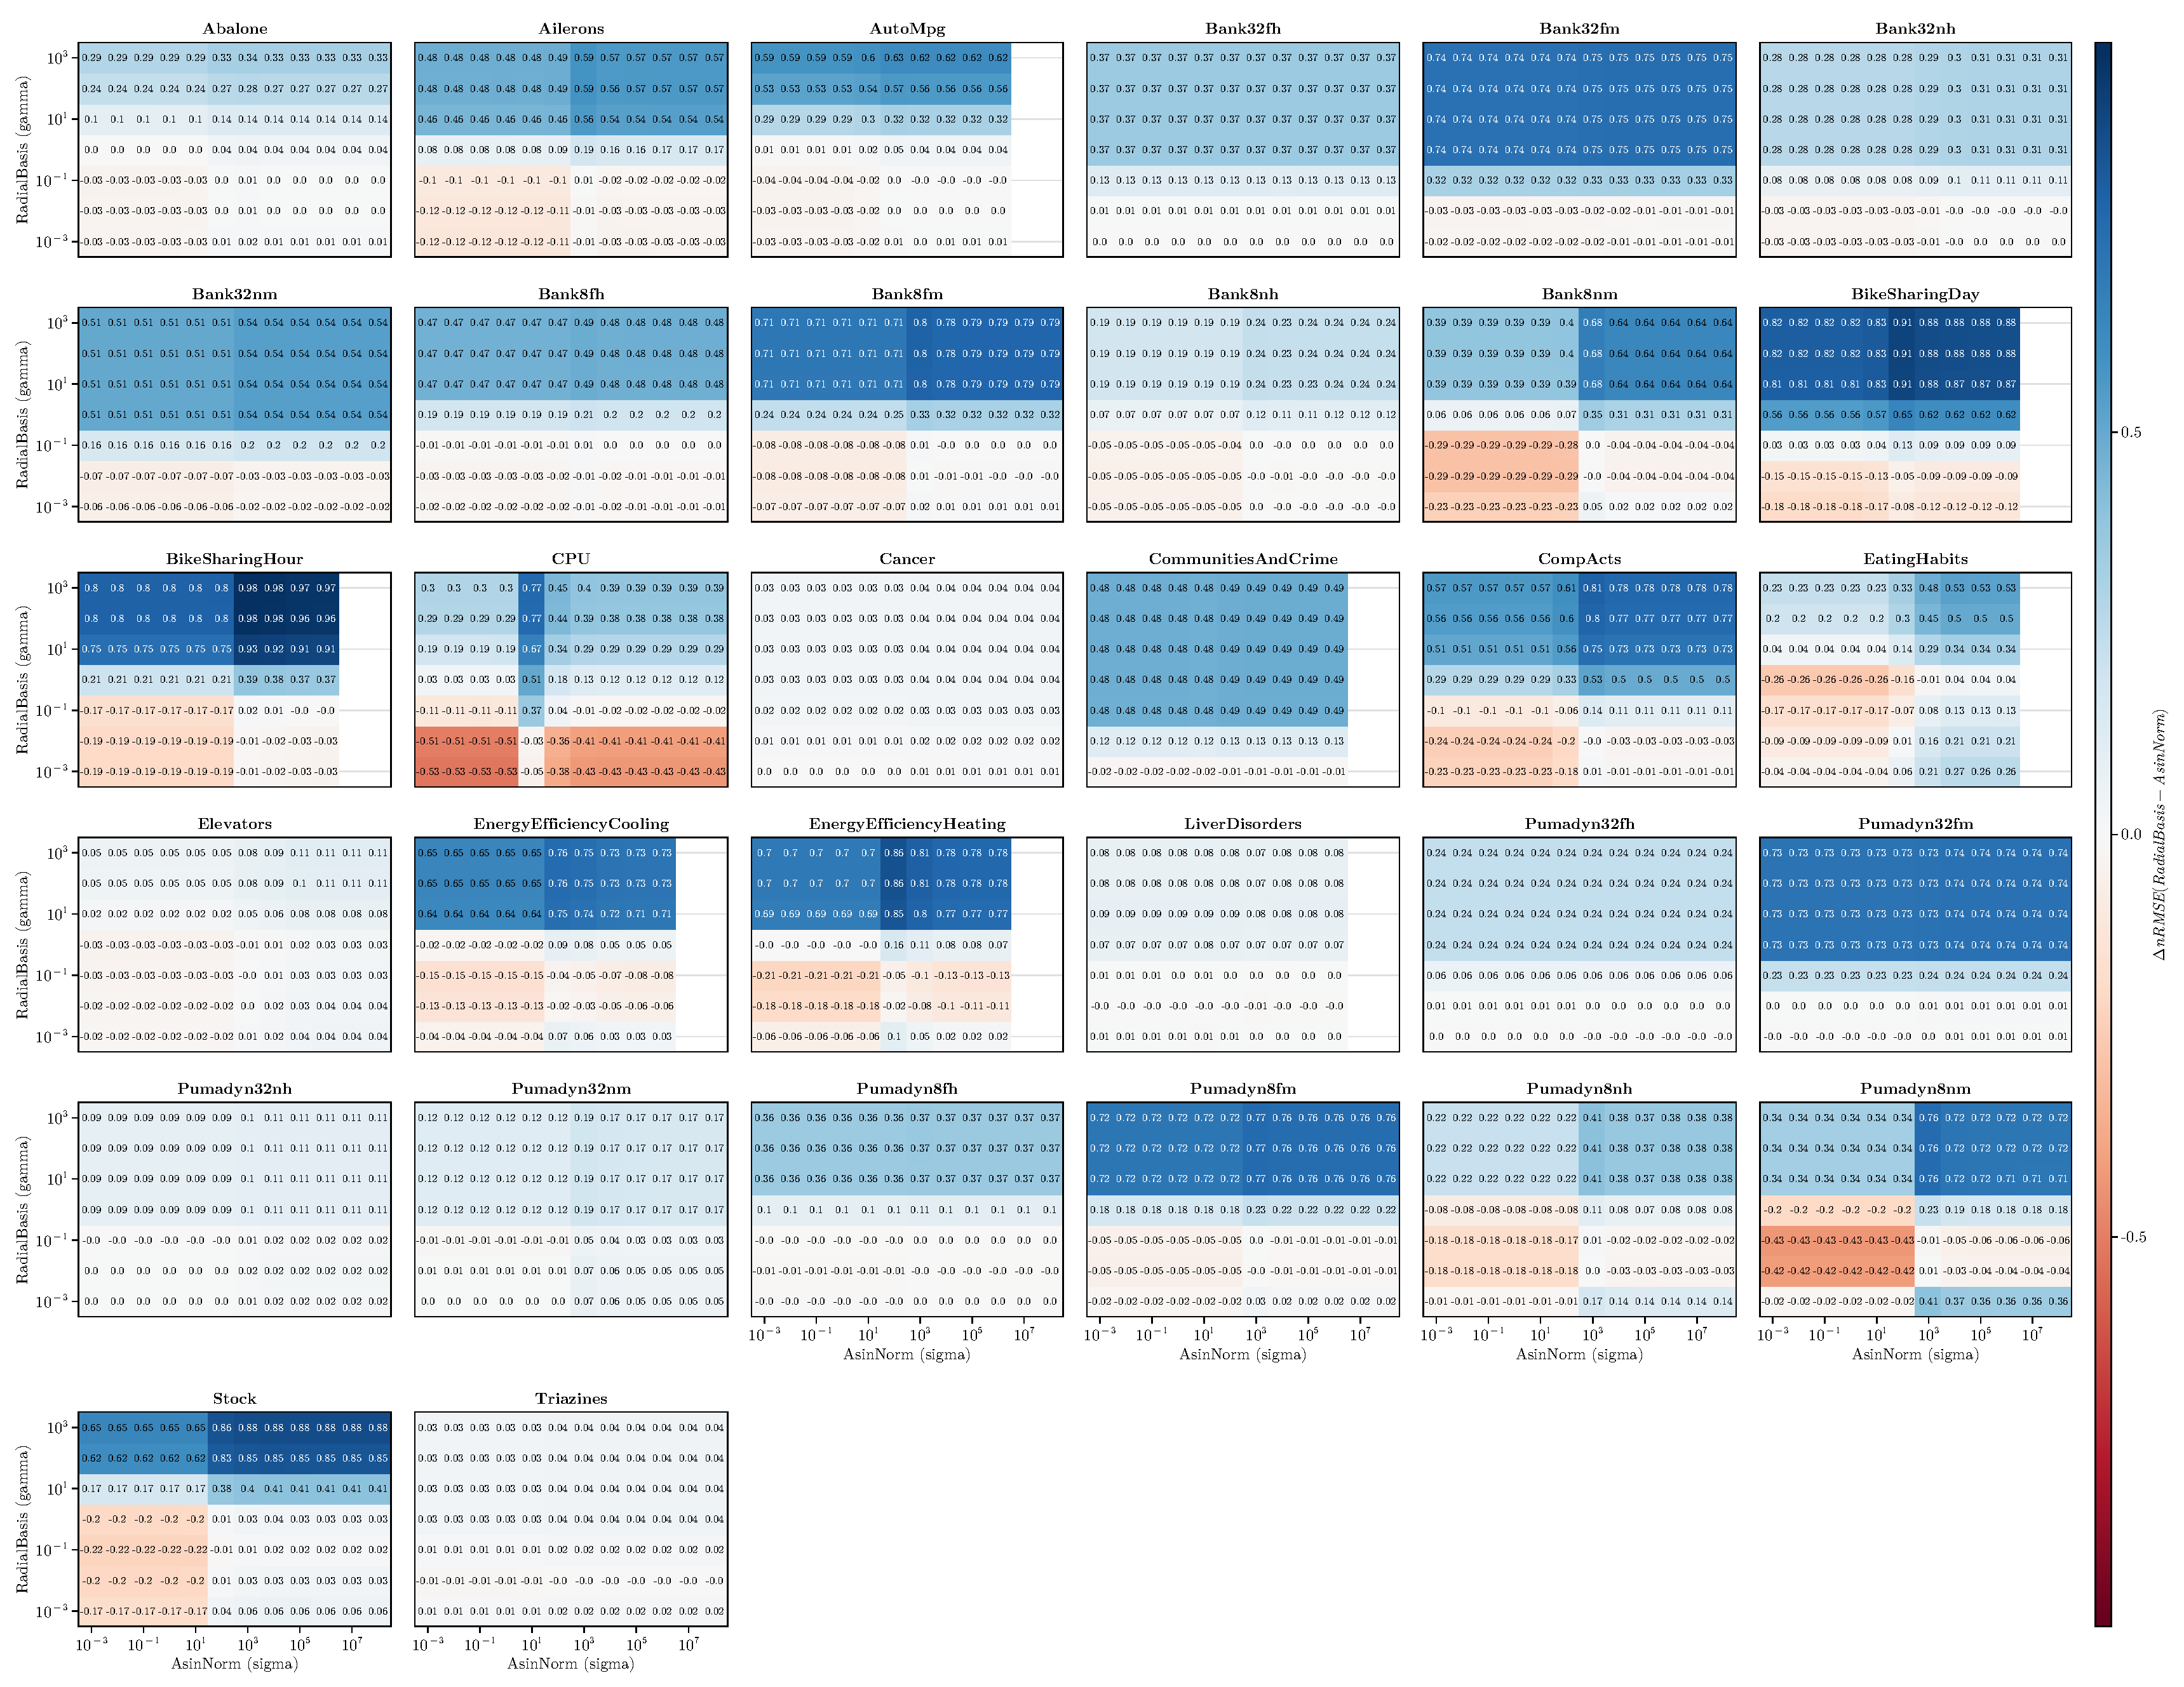
\includegraphics[width=0.9\textwidth]{plots/heatmaps_rbf_asinnorm}
%     \caption{Difference between nRMSE of RBF and normalized arc-sine kernels ($\alpha=0.001$)}
%     \label{fig:paired-ttest-rbf-asinnorm-diff}
% \end{figure}
%
% % \Cref{fig:heatmaps-rbf-asinnorm} shows the difference between the nRMSE of the
% % RBF and the normalized arc-sine kernel.
% %
% % Positive values (in blue) indicate that for that
% % combination of $\sigma_w$ and $\gamma$, the normalized arc-sine kernel
% % outperforms the RBF kernel.
% % Negative values (in red) indicate that the RBF
% % kernel performs better than the normalized arc-sine kernel.
% % The darker the color, the bigger the difference.
% %
% % We can observe 3 different behaviours:
% % \begin{itemize}
% %     \item The difference between the RBF and normalized arc-sine
% %           kernels is barely noticeable: \texttt{Cancer}, \texttt{LiverDisorders},
% %           \texttt{Triazines}, \dots. Looking at the results from the previous
% %           sections, these are \emph{hard} datasets, in the sense that the
% %           \emph{nRMSE} obtained by both the RBF and other kernels is high (>0.8).
% %
% %     \item There is no clear effect of $\sigma_w$ on the
% %           performance of the normalized arc-sine kernel: \texttt{Bank32fh},
% %           \texttt{Bank32fm}, \texttt{CommunitiesAndCrime}, \texttt{Pumadyn32fm}, \dots
% %
% %     \item There is threshold for $\sigma_w$ where the normalized
% %           arc-sine kernel goes from performing worse than the RBF kernel to
% %           performing equally or better than RBF.
% % \end{itemize}
% %
% % % TODO: explain better
% % Again, the \texttt{CPU} dataset exhibits a different behaviour where for
% % $\sigma_w=0.1$ it is able to match the performance of the RBF kernel, but
% % all the others it's significantly worse.
% %
% % \begin{figure}[H]
% %     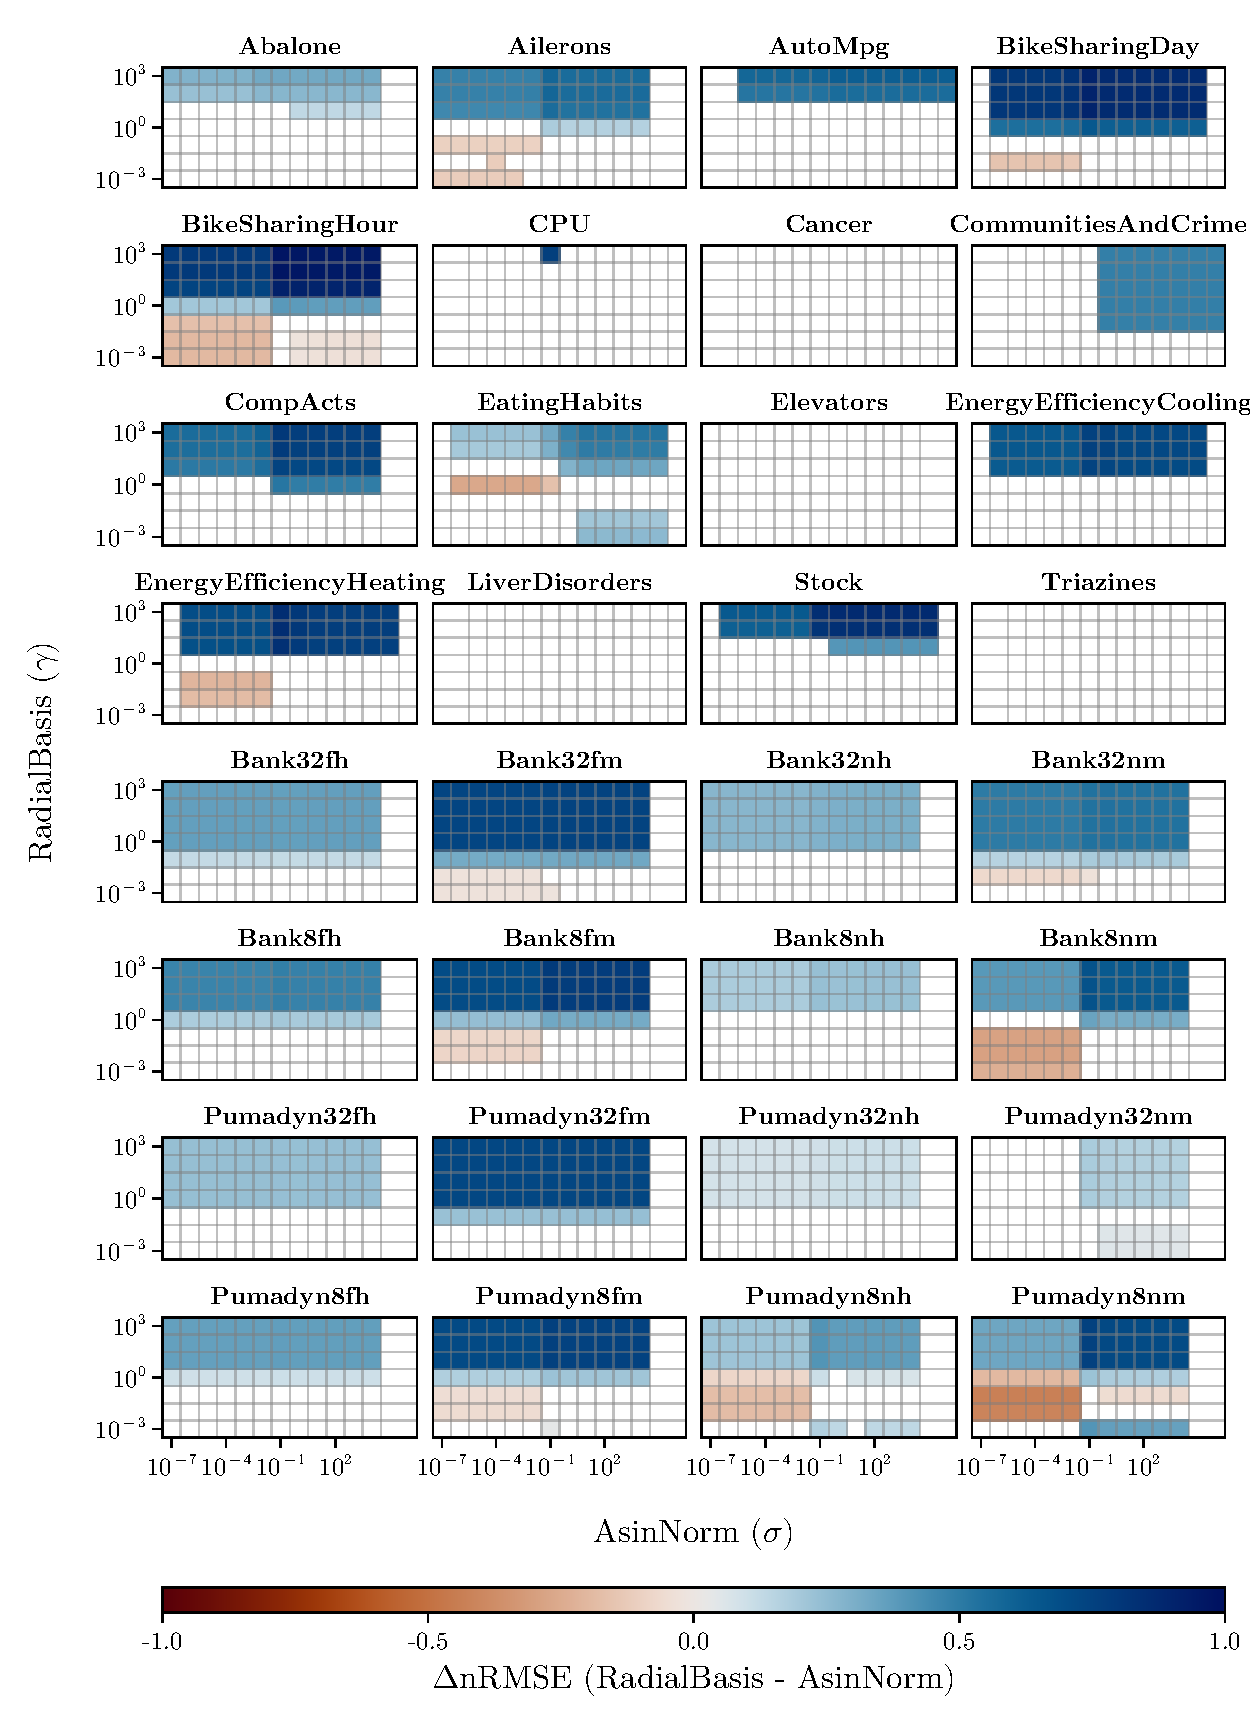
\includegraphics[width=0.9\textwidth]{plots/heatmaps_rbf_asinnorm_s}
% %     \caption{Difference between nRMSE of RBF and normalized arc-sine kernels}
% %     \label{fig:heatmaps-rbf-asinnorm}
% % \end{figure}
%
% \subsection{Arc-sine vs normalized arc-sine}
%
% \Cref{fig:heatmaps-asin-asinnorm} shows the $p$-values for the difference between
% the non normalized and the normalized arc-sine kernels. All datasets seem to have
% a region on the top right corner where the difference is not very significant.
% We can conjecture that for values of $\sigma$ big enough, the normalized and
% non-normalized arc-sine kernels perform similarly. The only notable exception is
% \texttt{BikeSharingHour}.
%
% \begin{figure}[H]
%     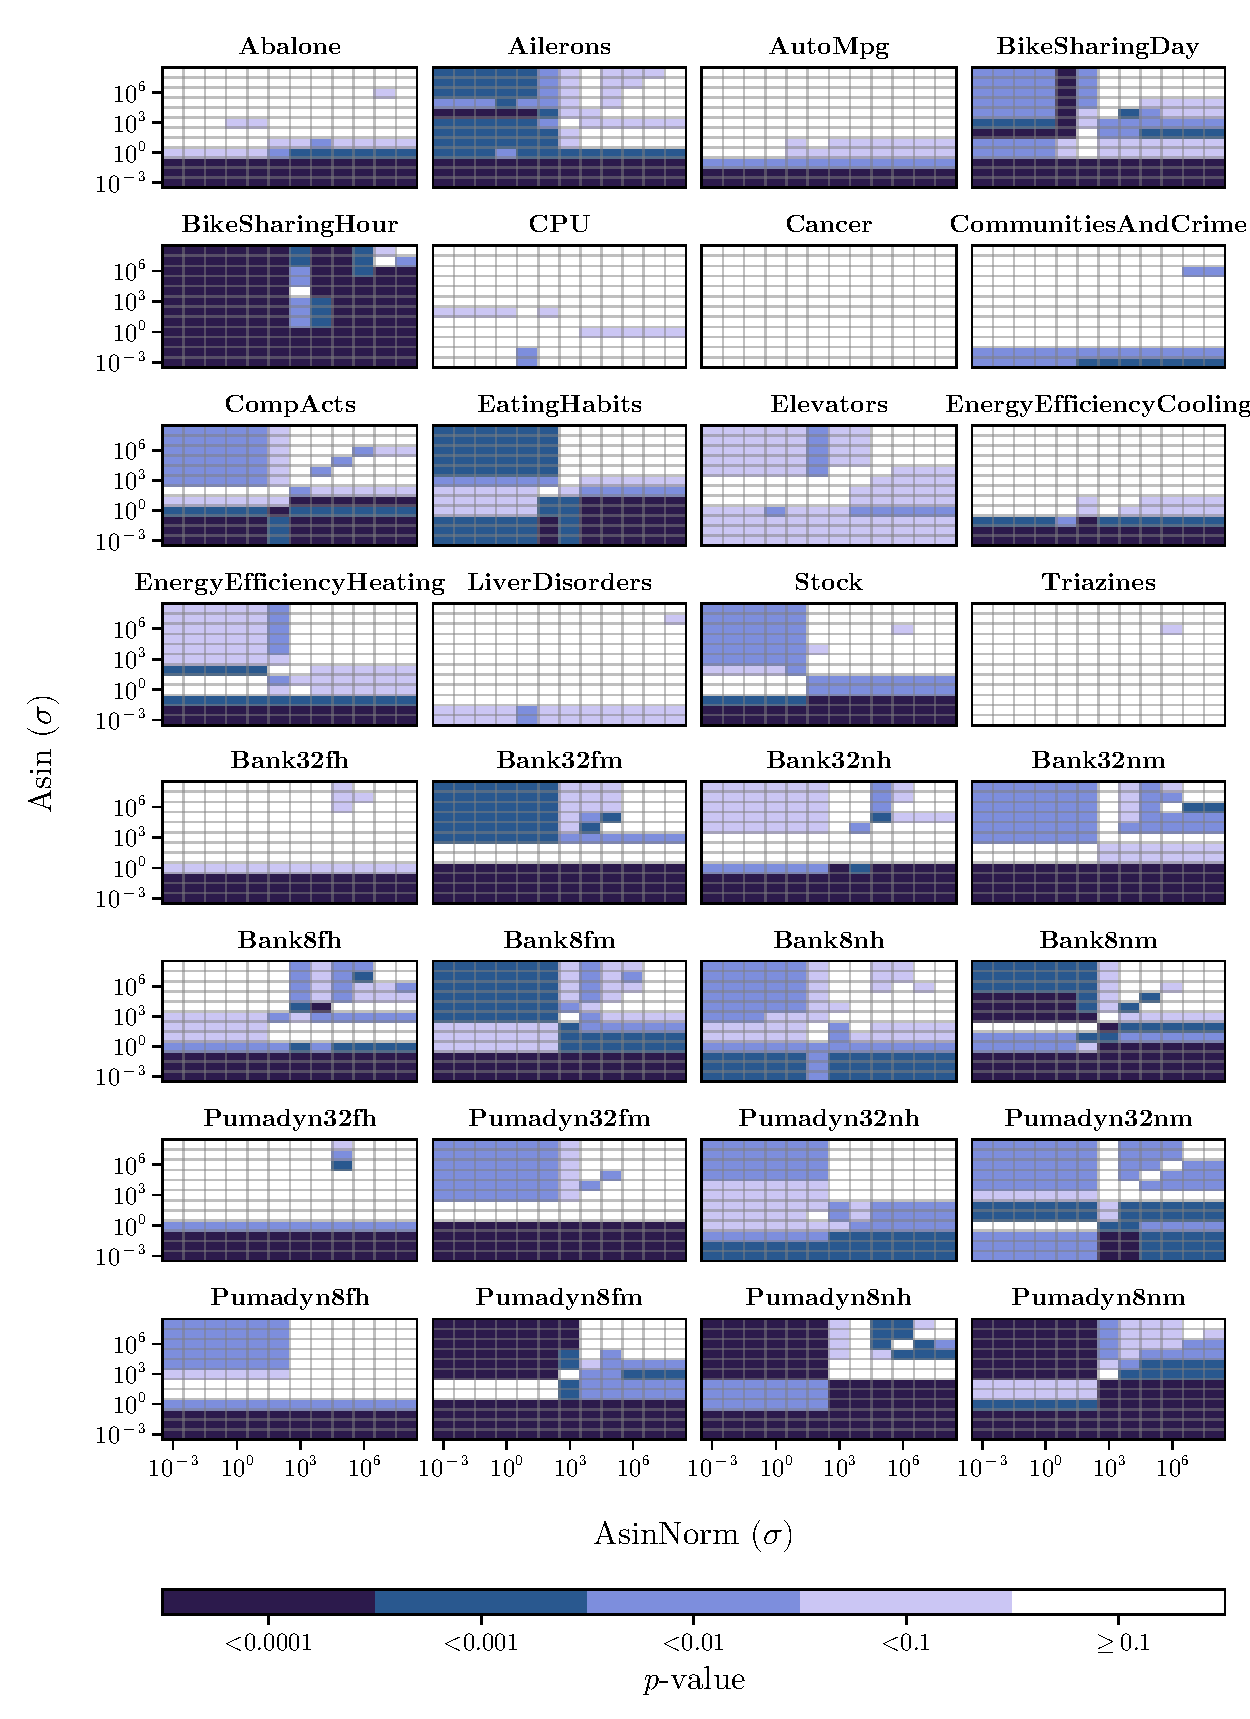
\includegraphics[width=0.9\textwidth]{plots/heatmaps_asin_asinnorm_pvalues}
%     \caption{Difference between nRMSE of arc-sine and normalized arc-sine kernels}
%     \label{fig:heatmaps-asin-asinnorm}
% \end{figure}
%
% \section{Training costs and drawbacks}
%
% All the analysis done so far has been based on the $nRMSE$ performance measure
% considering the best values of $\epsilon$ and $C$ for each dataset. However,
% the training cost of the SVM is also an important factor to consider.
%
% Indeed, we can conclude that under certain conditions, the rbf and arc-sine
% kernels perform similarly, but does the training time also match?
%
% While running the experiments, we measured both the training time and the
% number of iterations needed to train the SVM. These give more information
% about the cost of training the SVM than the $nRMSE$ alone.
%
% \begin{cnote}
%     Below are some RAW plots of the training time and number of iterations
%     from the best models of each kernel and dataset combination.
% \end{cnote}
% \begin{figure}[H]
%     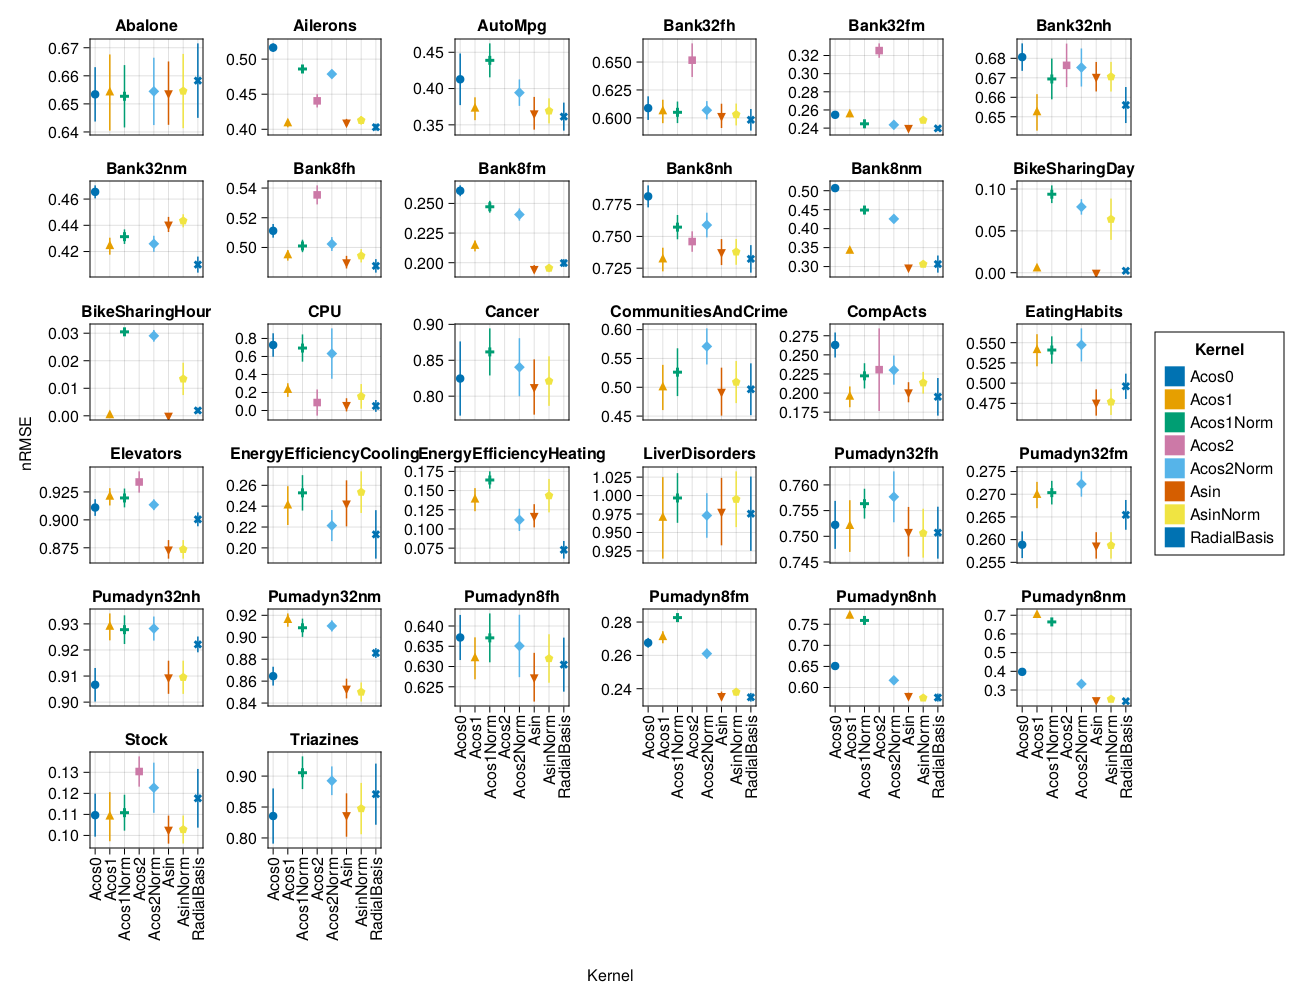
\includegraphics{raw_kernel_rmse_best}
%     \caption{Best $nRMSE$}
% \end{figure}
% \begin{figure}[H]
%     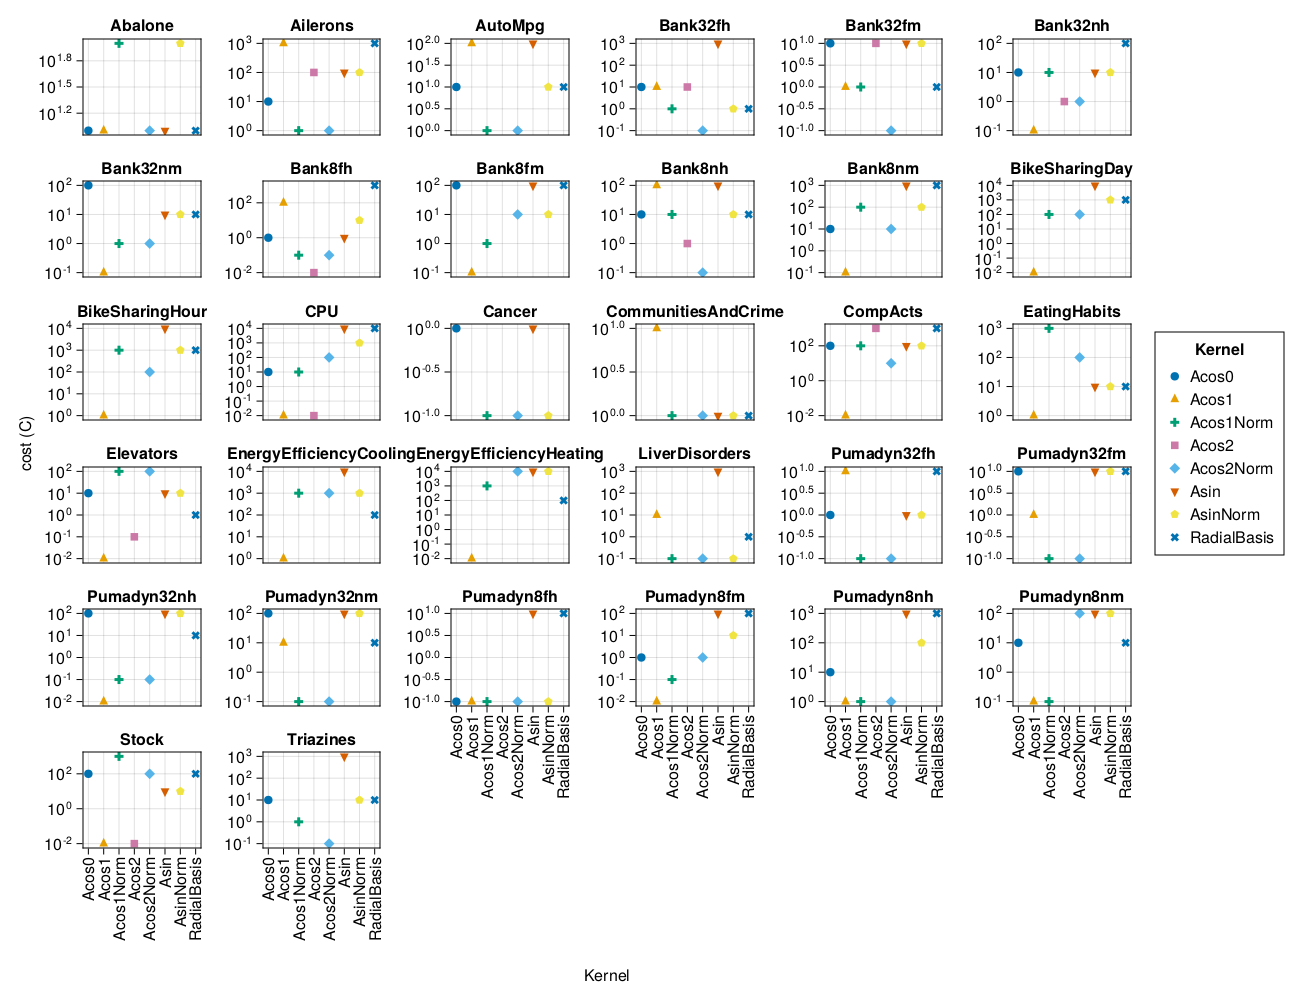
\includegraphics{raw_kernel_cost_best}
%     \caption{Best $nRMSE$ Cost parameter}
% \end{figure}
% \begin{figure}[H]
%     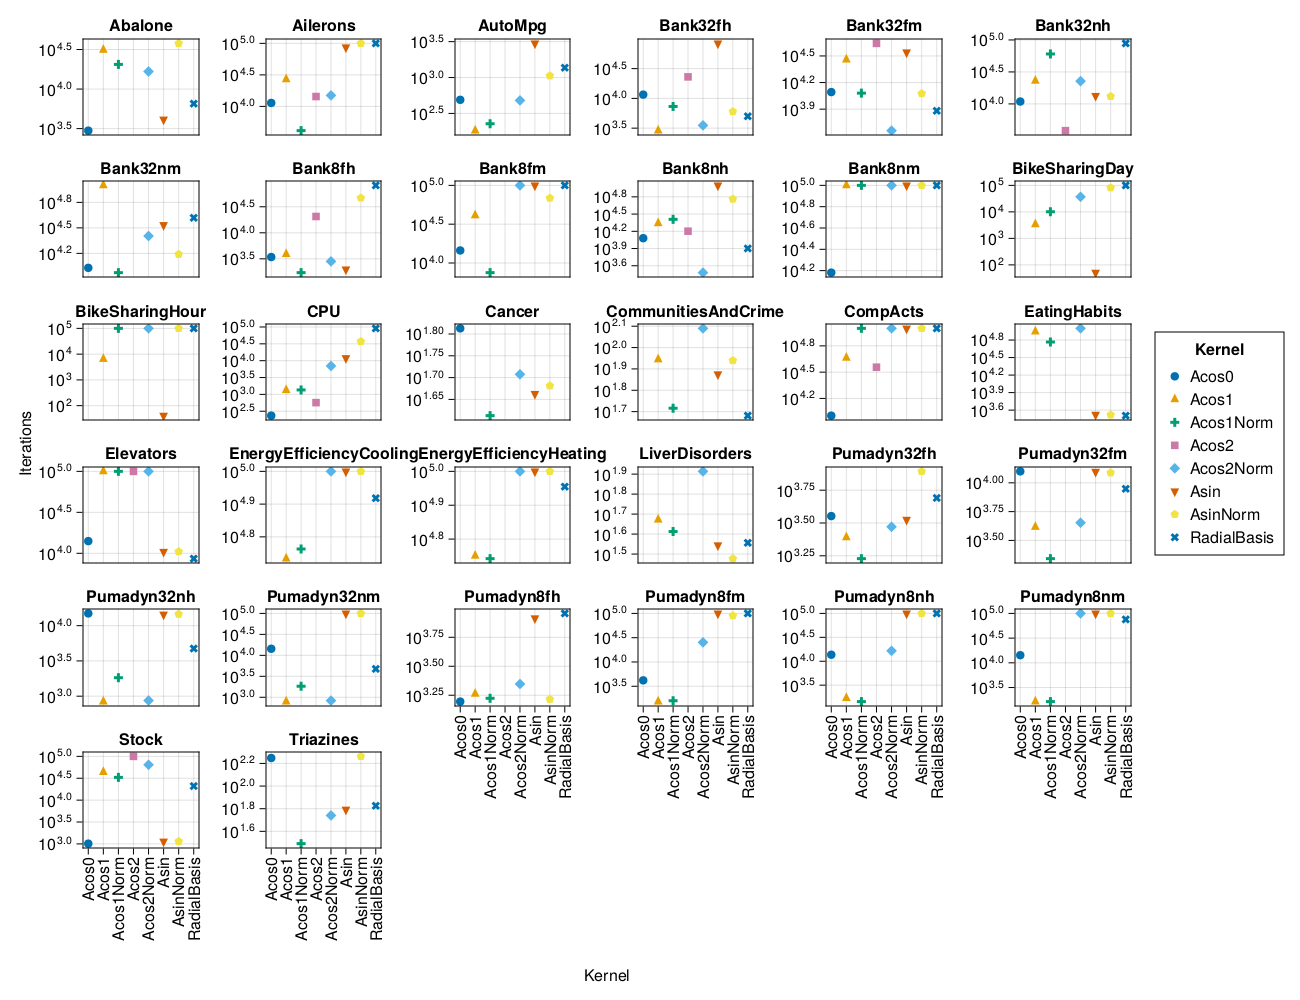
\includegraphics{raw_kernel_iterations_best}
%     \caption{Number of iterations for the best models}
% \end{figure}
% \begin{figure}[H]
%     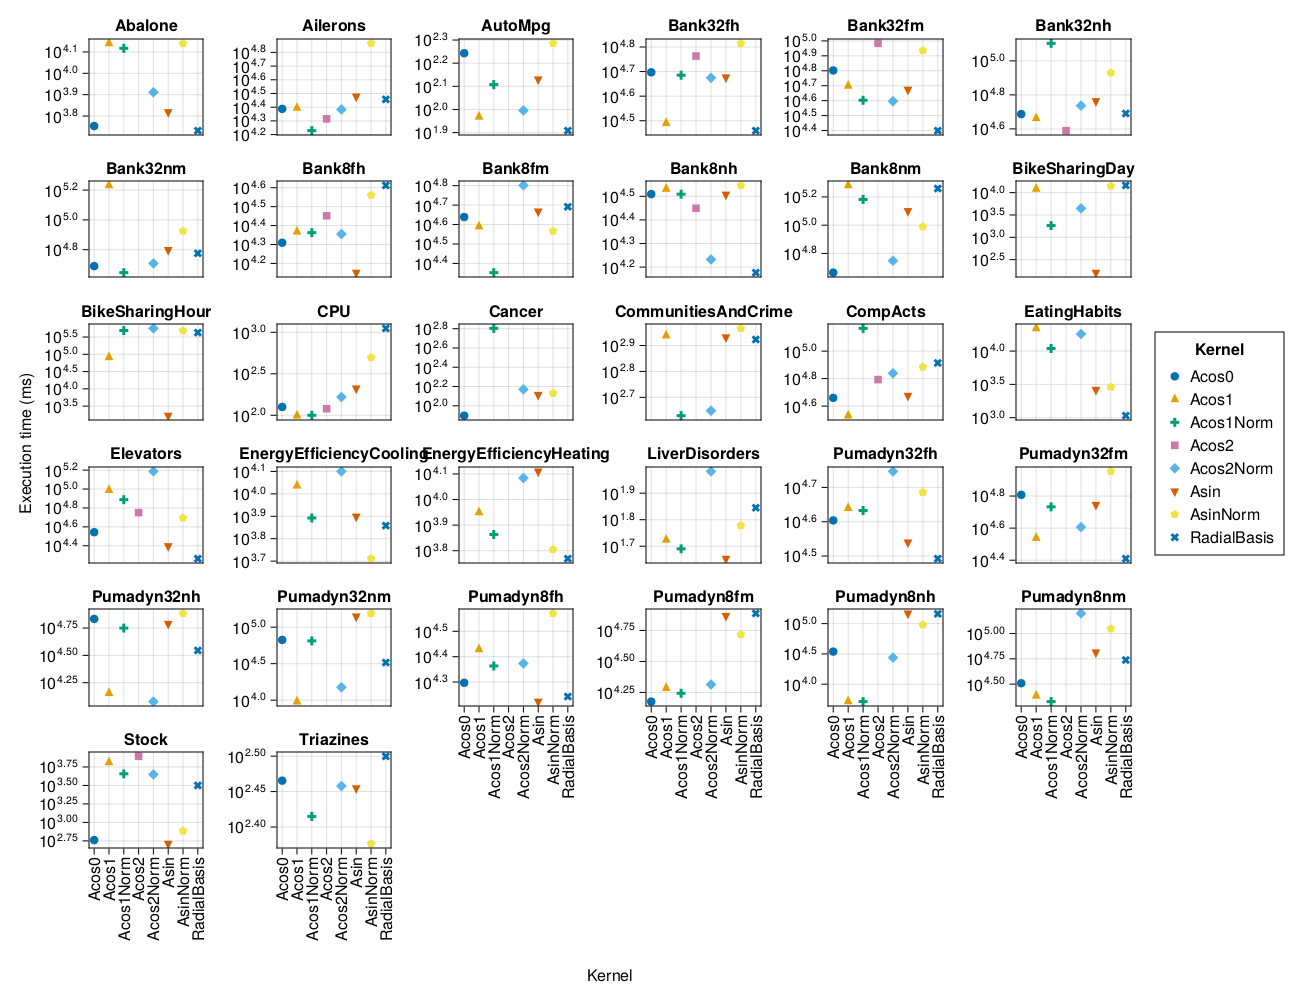
\includegraphics{raw_kernel_time_best}
%     \caption{Training time for the best models}
% \end{figure}
%
% % TODO: maybe a combination plot of the heatmap and the line plot for some
% % interesting datasets?
%
% % TODO: classification is a mess
% % \section{Classification}
% %
% % \begin{figure}[H]
% %     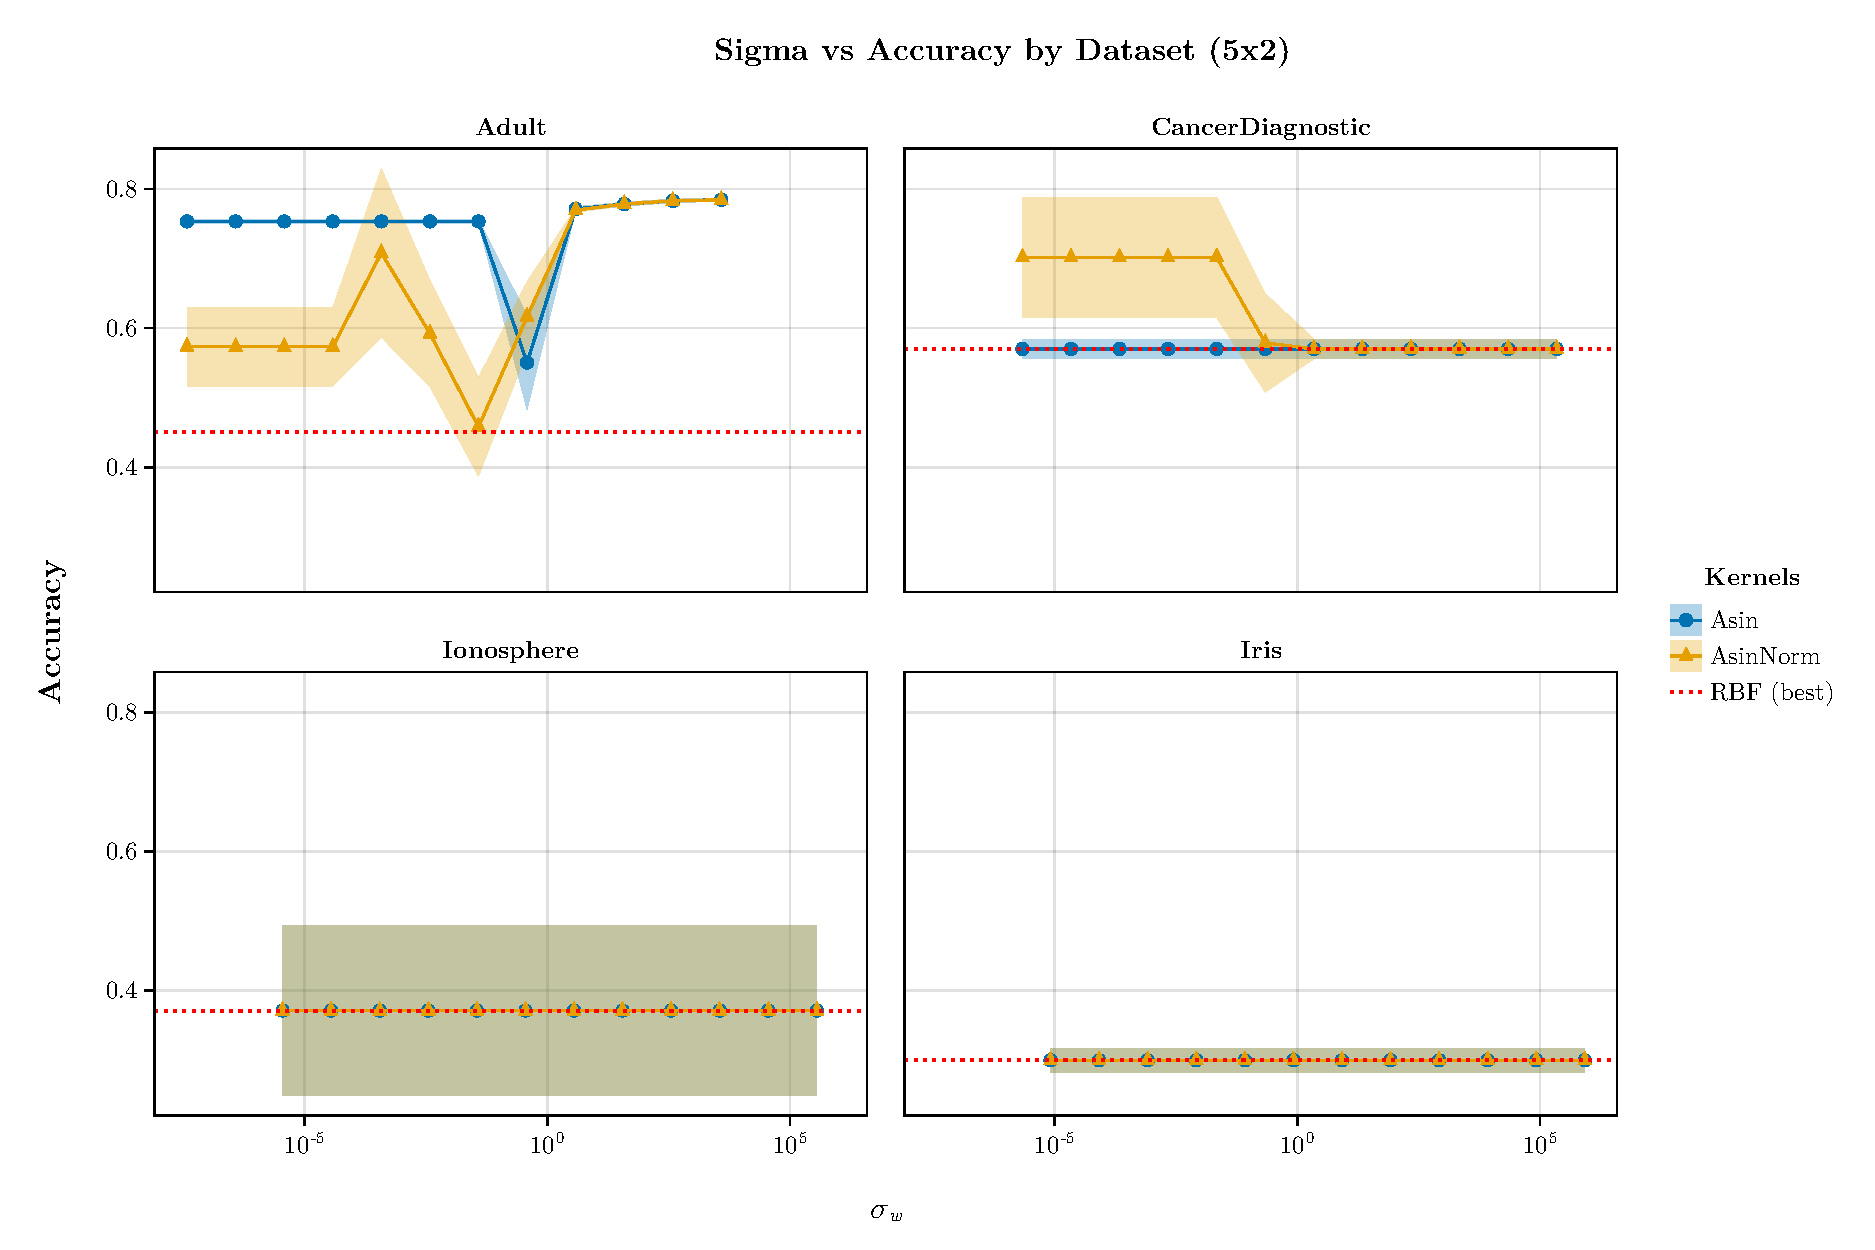
\includegraphics{plots/nRMSE_class_all_scaled}
% %     \caption{Classification accuracy}
% %     \label{fig:nrmse-class-all}
% % \end{figure}
% %
% % \begin{marker}
% %     This makes no sense, the accuracies are too low, specially iris (Even on the
% %     RBF).
% %
% %     Add the other datasets.
% %     Add more values of sigma.
% %     Other metrics (precision, recall, f1, etc)
% % \end{marker}
%
% % \section{Estimation of the time needed to train the SVM}
% %
% % The main incentive for using the arc-sine kernel is that it is supposed to be
% % parameter insensitive, which means that we can reduce the search space for the
% % hyperparameters and thus reduce the time needed to train the SVM.
% %
% % If for the RBF kernel we have to search for $n$ possible values of $\gamma$
% % hyperparameter whilst for the arc-sine kernel we can set $\sigma_w=10$ and
% % achieve similar results, then we can reduce the search space by a factor of $n$.
% %
% % However, it is still possible that even with a fixed $\sigma_w$ the arc-sine
% % kernel requires a wider search space for the other hyperparameters (cost and
% % $\varepsilon$) or the computation of the kernel is more expensive than the RBF
% % and thus the time needed to train the SVM is not reduced.
% %
% % For instance, in the initial testing of the normalized arc-sine kernel, the average
% % training for the Adult dataset using the normalized arc-sine kernel
% % took approximately 2 times longer than the RBF kernel.
%
% % TODO: plots de temps de execucio
% % TODO: plots de temps de iteracions / iteracions per segon
% % TODO: plots de temps de nombre de parametres provats
% %
%

\pagebreak
\section{Meta-learning}

As explained in \cref{sec:meta-learning}, we want to use meta-learning
techniques to determine the best value of sigma for a given dataset. That
is, we want to build a model which predicts the best value of sigma given
the properties of the dataset.

Since we have a very small number of datasets (32 for regression and 8 for classification)
we decided to use leave-one-out cross-validation to train the model. This
means that for each dataset, we train the model using all the other datasets
and then evaluate it on the dataset which was left out. This is repeated
for each dataset. The approach was used to tune the parameters of the model
and a 5-fold cross validation was used on top of that to evaluate the models.

We use the coefficient of determination ($R^2$) as the performance measure
for the model. Several models were tested, including ridge regression, lasso
regression, support vector regression, and random forest regression. However,
none of the models achieved a satisfactory performance. The best model was
a random forest regression with a coefficient of determination of $R^2=0.07$.

We explored other approaches to the problem, including doing random subsets of
different sizes for the datasets. Using this approach a 0.4 coefficient of
determination was achieved, however this was probably due to overfitting.

In general, the results obtained with meta-learning were not satisfactory, but
show a promising direction for future work. With a much larger group of datasets,
such approach could be used, and potentially by using explainable AI (XAI)
techniques, insight on which properties of the datasets are most relevant
to determine the best value of sigma could be obtained.
